%-----------------------
% Document initialization
%-----------------------
\documentclass{article}
\usepackage[utf8]{inputenc}
%--------------------
% Packages
% ------------------

%\usepackage[T2]{fontenc} - % måske noget med automatisk orddeling...
\usepackage{amsmath}
\usepackage{amsfonts}
\usepackage{extdash}
\usepackage{algorithm}
\usepackage{algpseudocode}
\newcommand{\algorithmautorefname}{Algorithm}

\usepackage[pdftex]{graphicx} % Required for including pictures
\usepackage[english]{babel} % using english
\usepackage[pdftex,linkcolor=black,pdfborder={0 0 0}]{hyperref} % Format links for pdf
\usepackage{calc} % To reset the counter in the document after title page
\usepackage{enumitem} % Includes lists
\usepackage[table,xcdraw]{xcolor} % colors
\usepackage{ctable}
\usepackage{sectsty} % Sectionstyles
\usepackage{titlesec}
\usepackage{epstopdf}
\usepackage{float}
\usepackage[font=small,labelfont=bf]{caption} % Bold label number
\usepackage{subcaption}
\counterwithin{figure}{section}
\usepackage{wallpaper}
\usepackage{hyperref}
\usepackage{framed}
\usepackage{multirow}

%%% Spacing and margins
\frenchspacing % No double spacing between sentences
\linespread{1.2} % Set linespace
\usepackage[top=3in, bottom=1.25in, left=1.25in, right=1.25in, headheight=25.0pt]{geometry}
\usepackage{parskip}
\setlength{\parindent}{1em}
\usepackage{cleveref}

\titleformat{\paragraph}
{\normalfont\normalsize\bfseries}{\theparagraph}{1em}{}
\titlespacing*{\paragraph}
{0pt}{3.25ex plus 1ex minus .2ex}{1.5ex plus .2ex}


% References
\usepackage[backend=biber,style=numeric,sorting=nty]{biblatex}
\addbibresource{MasterThesis.bib}
\usepackage{csquotes}

%\usepackage[all]{nowidow} % Tries to remove widows
%\usepackage[protrusion=true,expansion=true]{microtype} % Improves typography, load after fontpackage is selected

\usepackage{lipsum} % Used for inserting dummy 'Lorem ipsum' text into the template

%-----------------------
% Set pdf information and add title, fill in the fields
%-----------------------
\hypersetup{ 	
pdfsubject = {Master Thesis},
pdftitle = {MasterThesis2020},
pdfauthor = {Tobias Engelhardt Rasmussen}
}

%--------------------
% Setting up different page styles
% ------------------
\usepackage{fancyhdr}
\pagestyle{fancy}
\fancyheadoffset{0 cm}

\usepackage{afterpage}
% Blank-page page style
\newcommand\blankpage{%
    \null
    \thispagestyle{plain}%
    %\addtocounter{page}{0}%
    \newpage}
% Emptyhead
\fancypagestyle{emptyhead}{
  \fancyhf{}
  \fancyhead[L]{}
  \fancyhead[R]{}
  \cfoot{\thepage}
}
\fancypagestyle{emptyleft}{
  \fancyhead[L]{}
  \cfoot{\thepage}
}
\fancypagestyle{abstract}{
  \fancyhead[R]{\huge \textbf{Abstract}}
  \cfoot{\thepage}
}

\fancypagestyle{preface}{
  \fancyhead[R]{\huge \textbf{Preface}}
  \cfoot{\thepage}
}

\fancypagestyle{abbreviations}{
  \fancyhead[L]{\huge \textbf{List of Abbreviations}}
  \fancyhead[R]{}
  \cfoot{\thepage}
}

\fancypagestyle{symbols}{
 \fancyhead[L]{}
 \fancyhead[R]{\huge \textbf{Nomenclature}}
 \cfoot{\thepage}}

\fancypagestyle{contents}{
  \fancyhead[L]{}
  \fancyhead[R]{\huge \textbf{Contents}}
  \cfoot{\thepage}
}

\fancypagestyle{lof}{
  \fancyhead[L]{\huge \textbf{List of Figures}}
  \fancyhead[R]{}
  \cfoot{\thepage}
}

\fancypagestyle{lot}{
  \fancyhead[L]{}
  \fancyhead[R]{\huge \textbf{List of Tables}}
  \cfoot{\thepage}
}

\fancypagestyle{references}{
  \fancyhead[L]{}
  \fancyhead[R]{\slshape\leftmark}%
  \cfoot{\thepage}
}

\fancypagestyle{main}{%
  \fancyhf{}%
  \fancyhead[R]{\slshape\leftmark}%
  \fancyhead[L]{\slshape\rightmark}%
  \fancyfoot[C]{\thepage}%
  \renewcommand{\headrulewidth}{0.4pt}%
  %\renewcommand{\footrulewidth}{0.4pt}%
}






% New commands  %%%%%%%%%%%%%%%%%%%%%%%%%%%%%%%%%%%%%%%%%%%%%%%%%%%%%%%%%%%%%%
% Bold symbols
\newcommand{\bs}{\boldsymbol}
\newcommand{\R}{\mathbb{R}}
\newcommand{\tensor}{\mathcal}


%-----------------------
% Begin document
%-----------------------
\begin{document}

% Block commenting starting here !! (ends with \fi)
%\iffalse

\newgeometry{top = 2in}

% FRONTPAGE %%%%%%%%%%%%%%%%%%%%%%%%%%%%%%%%%%%%%%%%%%%%%%%%%%%%%%%%%%%%%%%%%%%%%%%%%%%%
\begin{titlepage}

\newcommand{\HRule}{\rule{\linewidth}{0.5mm}} % Defines a new command for the horizontal lines, change thickness here

\center % Center everything on the page
 
%----------------------------------------------------------------------------------------
%	HEADING SECTIONS
%----------------------------------------------------------------------------------------



\textsc{\LARGE Technical University of Denmark}\\[0.5cm] % Name of your university/college

\begin{figure}[h]
\begin{center}

\includegraphics[width=2cm]{Pics/frontpage/dtu_logo.png}
\end{center}
\end{figure}

\textsc{\Large Master Thesis in Mathematical Modelling and Computation}\\[0.5cm] % Major heading such as course name

%----------------------------------------------------------------------------------------
%	TITLE SECTION
%----------------------------------------------------------------------------------------

\HRule \\[0.4cm]
{ \huge \bfseries Evaluation of synergistic effects of tensor decomposition methods within (deep) neural network applications}\\[0.4cm] % Title of your document
\HRule\\ [1cm]
 


%----------------------------------------------------------------------------------------
%	AUTHOR SECTION
%----------------------------------------------------------------------------------------

%\begin{minipage}{0.5\textwidth}
%\begin{flushleft} \large
%\textbf{Group members:}\\
\begin{center}
\large Tobias Engelhardt \textsc{Rasmussen}, s153057 % Your name
\end{center}
%\end{flushleft}
%\end{minipage}
%\begin{minipage}{0.4\textwidth}
%\begin{flushright} \large
\vspace{1cm}
\begin{center}
\large \textbf{Supervisors} \\
\begin{tabular}{ll}
   \large Andreas \textsc{Baum}  & (andba@dtu.dk)  \\
   \large Line Katrine Harder \textsc{Clemmensen}  & (lkhc@dtu.dk) 
\end{tabular}
\\[5cm]
{\large January 2021}\\[3cm]
\end{center}
 % Date, change the \today to a set date if you want to be precise
%\end{flushright}
%\end{minipage}\\[1cm]

% If you don't want a supervisor, uncomment the two lines below and remove the section above
%\Large \emph{Author:}\\
%John \textsc{Smith}\\[3cm] % Your name
%----------------------------------------------------------------------------------------
%	DATE SECTION
%----------------------------------------------------------------------------------------



%----------------------------------------------------------------------------------------
%	LOGO SECTION
%----------------------------------------------------------------------------------------

%\includegraphics{Logo}\\[1cm] % Include a department/university logo - this will require the graphicx package
 
%----------------------------------------------------------------------------------------

%\vfill % Fill the rest of the page with whitespace

\end{titlepage}

\thispagestyle{empty}
\ThisLLCornerWallPaper{0.8}{Pics/frontpage/DTU-frise-SH-15_2.pdf}
\vspace*{\fill}

\noindent Technical University of Denmark \\
Department of Applied Mathematics and Computer Science \\
Richard Petersens Plads, building 324 \\
2800 Kongens Lyngby, Denmark \\
Phone +45 4525 3031 \\
compute@compute.dtu.dk \\ 
www.compute.dtu.dk \\
\clearpage

\restoregeometry

% Starting roman numbering
\setcounter{secnumdepth}{0}
\pagenumbering{Roman}

\sectionfont{\color{white}}


% ABSTRACT %%%%%%%%%%%%%%%%%%%%%%%%%%%%%%%%%%%%%%%%%%%%%%%%%%%%%%%%%%%%%%%%%%%%%%%%%%%%%
\afterpage{\blankpage}
\thispagestyle{abstract}
This paper examines... Something very interesting

\clearpage

% PREFACE %%%%%%%%%%%%%%%%%%%%%%%%%%%%%%%%%%%%%%%%%%%%%%%%%%%%%%%%%%%%%%%%%%%%%%%%%%%%%%
%\afterpage{\blankpage}
\thispagestyle{preface}
\section{Preface}

\noindent This Master Thesis; "Evaluation of synergistic effects of tensor decomposition methods within (deep) neural network applications" is conducted in order to fulfill the requirements for achieving the Master of Science in Engineering; Mathematical Modelling and Computing. The work is done in the fall semester of 2020 at the Department of Applied Mathematics and Computer Science (DTU Compute) at the Technical University of Denmark in Kongens Lyngby. The project was supervised by Andreas Baum, Assistant Professor, and Line Katrine Harder Clemmensen, Associate Professor, both at DTU Compute.

\vspace{4cm}
\begin{flushright}
Kongens Lyngby, January 2021 \\
\vspace{2cm}

\begin{tabular}{ll}
         &                   \\ \hline
         &                    \\
 & Tobias Engelhardt Rasmussen
\end{tabular}

\end{flushright}

\clearpage

% Decreasing top margin
\newgeometry{top = 2in}

% CONTENTS %%%%%%%%%%%%%%%%%%%%%%%%%%%%%%%%%%%%%%%%%%%%%%%%%%%%%%%%%%%%%%%%%%%%%%%%%%%%%
\thispagestyle{contents}
\setcounter{tocdepth}{4}
\tableofcontents
\clearpage

% List of Tables %%%%%%%%%%%%%%%%%%%%%%%%%%%%%%%%%%%%%%%%%%%%%%%%%%%%%%%%%%%%%%%%%%%%%%%
\section{List of Figures}
\thispagestyle{lof}
\listoffigures
\clearpage

% List of figures %%%%%%%%%%%%%%%%%%%%%%%%%%%%%%%%%%%%%%%%%%%%%%%%%%%%%%%%%%%%%%%%%%%%%%
\section{List of Tables}
\thispagestyle{lot}
\listoftables
\clearpage

%\fi %finish commenting

% ABREVIATIONS %%%%%%%%%%%%%%%%%%%%%%%%%%%%%%%%%%%%%%%%%%%%%%%%%%%%%%%%%%%%%%%%%%%%%%%%%
\thispagestyle{abbreviations}
\section{List of Abbreviations}

\begin{description}[leftmargin=!,labelwidth=2cm]
    \item [VIP] Very Important Person
    \item [PC] Personal Computer
    \item [NN] Neural Network
    \item [CNN] Convolutional NN
    \item [hmm] Hmmmmmm
    \item [TNN] Tensorized NN

\end{description}

\clearpage

% Symbols %%%%%%%%%%%%%%%%%%%%%%%%%%%%%%%%%%%%%%%%%%%%%%%%%%%%%%%%%%%%%%
\thispagestyle{symbols}
\section{Nomenclature}

In this thesis, vectors will be denoted as bold lower case letters $\boldsymbol{x}$, while bold upper case letters denote matrices $\bs{X}$, with elements $\bs{X}(i, j) = x_{i,j}$. Tensors of dimension at least 3 are written in calligraphic letters, hence $\mathcal{X}^{d_1\times d_2 \times \dots \times d_N}$ is a tensor of order $N$ with elements $\tensor{X}(i_1, i_2, \dots, i_N) = x_{i_1, i_2, \dots, i_N}$. A list of symbols used throughout the thesis is given below. 

\vspace{1cm}

\begin{tabular}{cll}
    \textbf{Symbol} & \textbf{Description} & \textbf{Operation}  \\ \hline
    & & \\
    $\langle \mathcal{A}, \mathcal{B}\rangle$ & Inner product & $\langle \mathcal{A}, \mathcal{B}\rangle = \sum_{i,j,k} a_{i,j,k}\cdot b_{i,j,k}$ \\[2ex]
    $\circ$ &  Outer product & $\boldsymbol{a} \circ \boldsymbol{b} = \boldsymbol{C}$ where $c_{i,j} = a_i \cdot b_j$ \\[2ex]
    $\| \mathcal{A} \|_F$ & Frobenius norm & $\sqrt{\langle \mathcal{A}, \mathcal{A}\rangle}$ \\[2ex]
    $\bs{X}_{(n)}$ & Matricizing & $\tensor{X}^{I_1 \times I_2 \times \dots I_N} \longrightarrow \bs{X}_{(n)}^{I_n \times I_1 \cdot I_2 \cdots I_{n-1} \cdot I_{n+1} \cdots I_N}$ \\[2ex]
    $\times_n$ & $n$-mode product & $\tensor{X}\times_n \bs{M} = \tensor{Z}$ where $\bs{Z}_{(n)} = \bs{M}\bs{X}_{(n)}$ \\[2ex]
    $\otimes$ & Kronecker product & $\bs{A}\otimes \bs{B} = \bs{C}$ where $\bs{C}\left(k + K(i-1), l + L(j-1)\right) = a_{ij} \cdot b_{kl}$ \\[2ex]
    $\bs{X}^{\dagger}$ & Moore-penrose inverse & $\bs{X}^{\dagger} = ( \bs{X}^\top \bs{X})^{-1}\bs{X}^{\top}$ \\[2ex]
    $\odot$ & Khatri-Rao product & $\bs{A} \odot \bs{B} = \bs{C}$ where $\bs{C}\left(k + K(i-1), j\right) = a_{ij}b_{kj}$
\end{tabular}
\clearpage

% Going back to arabic numbering
\setcounter{secnumdepth}{4} %Means that 4 levels of sectioning comes into the table of contents
\pagenumbering{arabic}
\setcounter{page}{1}
% Setting section color and top margins
\newgeometry{top = 1.25in}
\sectionfont{\color{black}}
\pagestyle{main}


% Sections %%%%%%%%%%%%%%%%%%%%%%%%%%%%%%%%%%%%%%%%%%%%%%%%%%%%%%%%%%%%%%%%%%%%%%%%%%%%
%\section{Introduction} \label{tex:introduction}

Machine Learning (ML) has been a very useful tool in many areas for a long time. One of the biggest leaps in the discovery of the computer was Alan Turing's learning machine that was used to decrypt the German cipher during World War II \cite{turing}. Alan Turing was widely considered the father of computer science and artificial intelligence\cite{Beavers2013}. Ever since his work and with computers becoming better and more accessible, people have studied different ways of making machines learn different tasks. Today ML is used for everything from recognising handwriting to diagnosing breast cancer\cite{Khuriwal2018}. 

One of the most famous and versatile ML algorithms is the neural network (NN), which builds upon the idea of the brain with neurons firing up and sending information to each other through a network. NNs are very powerful since they are easy to train (finding the optimal weights), and easy to modify to fit almost any given problem. This means that NNs achieve state-of-the-art performance in a large variety of problems. Artificial neural networks (ANNs) are simply a set of neurons arranged in layers sending information from one layer to another from the input to the output. Stacking multiple layers of neurons makes the algorithm able to extract higher level features\cite{deepLearning}, hence many layers (deep learning) are often preferred for complex problems.

A big area in ML and NN research is image classification and detection, which is respectively to classify an image into a set of predetermined classes or detect a given object in an image. By far the major method in learning images is the convolutional neural network (CNN). In a CNN a number of filters are trained and run through the image to calculate activations. These filters will then be trained to see different features in the image such as lines or curves. Stacking multiple layers of convolutions enables the algorithm to learn more abstract features such as faces, printed text or wrinkly clothes\cite{Yosinski2015}. CNNs are the preferred NN architectures for image analysis, since they keep achieving state-of-the-art performance.

\subsection{The problem}
Even though NNs are very powerful and there is nothing to be said about their ability to learn, there is one problem. The amount of parameters to be trained and the amount of time it takes grow rapidly as the number of layers and the amount of neurons in these layers grow. The amount of parameters grow exponentially as the input resolution increases. For instance the MNIST data set, which consists of $28\times28$ pixel values per image will need $28\cdot28 = 784$ input neurons. If one is to have a fully connected (dense) layer from these inputs to another layer of just 100 neurons, the amount of parameters to be trained is $784 * 100 + 100 = 784,100$ (there is one bias term per neuron). Denil et al. found in 2013 that many of the weights in a deep NN are redundant\cite{Denil2013}. They found that if only a fraction of the weights were trained and the rest predicted from these, they would get close to the same accuracy as a fully trained network. This means that a high accuracy should be obtainable from a network with fewer parameters, if the architecture and algorithm itself are chosen wisely.

Many approaches have been attempted to solve this problem. For instance Liu et al. in 2015 used pruning to zero-out\footnote{Setting insigificant parameters to 0 (parameters that are already relatively close to 0)} more than 90 \% of the learned parameters with a loss in accuracy of under 1\% on a given data set. There have been many attempts to use tensor decomposition to reduce the number of parameters. Tensor decomposition is a way of approximating a multi-dimensional data array using a limited amount of parameters by looking at the variation in different dimensions. Numerous approaches have been generalizing this concept to change the architecture as in the work of Lebedev et al. in \cite{Lebedev2015} and of Wang et al. in 2016 \cite{Wang2016}. These methods decompose the weights of a pre-trained network and use the decompositions in the new architecture. After fine-tuning the performance should be increased both with respect to the number of parameters and the computation time, while the accuracy should remain approximately the same.

\subsection{Aim of this project}
This thesis investigates previous attempts and other potential approaches to evaluate the potential synergistic effects of using these methods within a deep NN. The aim is to examine the effects of using different tensor decomposition methods either before (as input) or within a potentially deep NN. The methods will be investigated and compared to baseline results in order to analyze the accuracy, running times, and number of parameters. Two data sets will be used to assess the performance differences. The first is the rather simple MNIST (Modified National Institute of Standards and Technology) data set\cite{MNIST}, which consists of handwritten digits from 0 to 9. The other is the THETIS (Three dimEnsional TennIs Shots) data set \cite{Gourgari2013}, which consists of videos of individuals performing different types of tennis shots. The purpose is to first apply the methods to the simpler MNIST data set, since this is well-studied and relatively easy to work with, and then apply them to the more complicated THETIS data set in order to test the methods on a more demanding problem. In appropriate cases the well-known VGG-16 network will be applied in order to check the performance of the given method on a well-known NN.
%\clearpage

\section{Theory} \label{tex:theory}
In this section, the theory used to develop the methods and obtain the result in this thesis will be discussed. First, neural networks (NNs) will be covered - both the simpler artificial NNs (ANNs) and more complex networks such as the convolutional NN (CNN) in both 2 (image) and 3 (videos) dimensions. Also methods for calculating the theoretical speed of a NN will be covered. This is followed by the theory behind tensors and different methods in tensor decomposition. There will be more focus on Tucker decomposition since it is the one used in this thesis, and how to choose the appropriate rank in the case of Tucker decomposition.
\begin{figure}[H]
    \centering
    \captionsetup{width=.95\linewidth}
    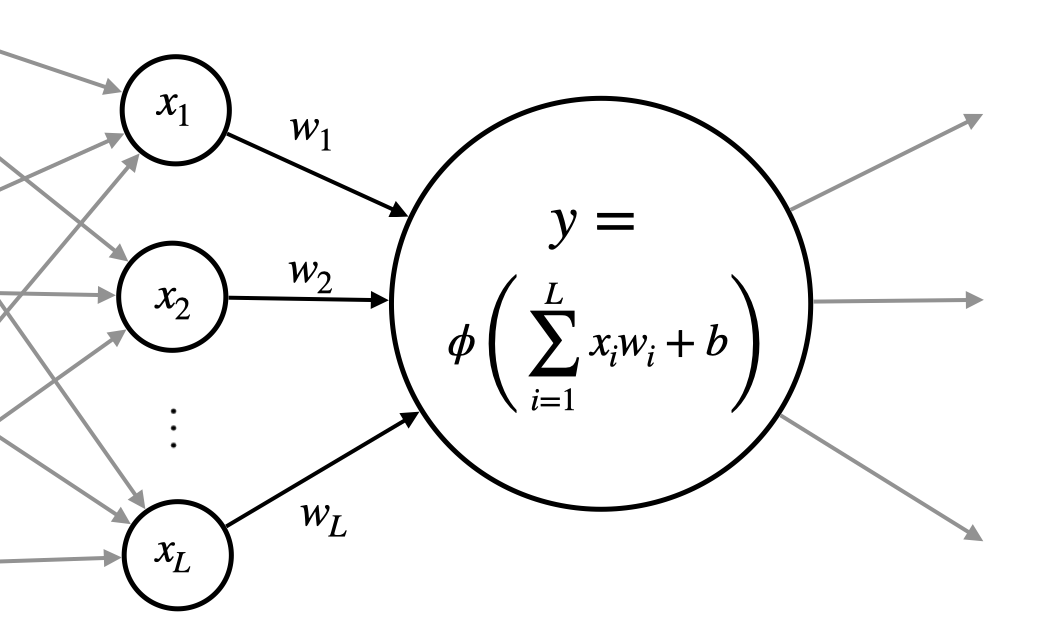
\includegraphics[width=.7\linewidth]{Pics/02_Theory/activation_illustration.png}
    \caption{Illustration of the flow of information through a neuron. Each edge (arrow) has a weight $w$ associated with it, and each neuron (circle) has an activation associated with it. The activations correspond to the information that is passed through the network, i.e. in this case the $L$ $x$s are used as inputs into the big neuron, where $y$ will be the resulting activation. $\phi$ is a non-linear transform called the activation function.}
    \label{fig:activation_illustration}
\end{figure}


\subsection{Neural Networks}\label{tex:theory_NN}
The NN is a very useful tool in non-linear classification and regression. It gets its name from what gave rise to the idea of it around half a century ago - the brain. Similar to the brain, a NN consists of a network of neurons that pass on information between each other. The way this is done is illustrated in \autoref{fig:activation_illustration}. Each neuron is, with a given input, associated with a value called its activation. This activation is based on the inputs to that very neuron, and is what is passed on from that neuron. The activation is calculated as the weighted sum of the activations of the inputs to that neuron plus a bias, all non-linearly transformed using an activation function $\phi$. Typical choices of $\phi$ are given in \autoref{fig:activation_functions}, while the typical activation of the last layer (the output) is the softmax-function, given by:
\begin{equation}
\text{Softmax:} \ \ \sigma: \R^K \rightarrow \R^K \qquad \sigma(\bs{x})_i = \frac{e^{x_i}}{\sum_{k=1}^K e^{x_k}} \quad \text{where} \ \bs{x} \in \R^K
\end{equation}
This is due to its ability to ensure a sum of 1 of all the outputs. In the end this value is the probability of the input belonging to each of the output classes. The predicted class is the one that has the highest probability.
\begin{figure}
    \centering
    \captionsetup{width=.95\linewidth}
    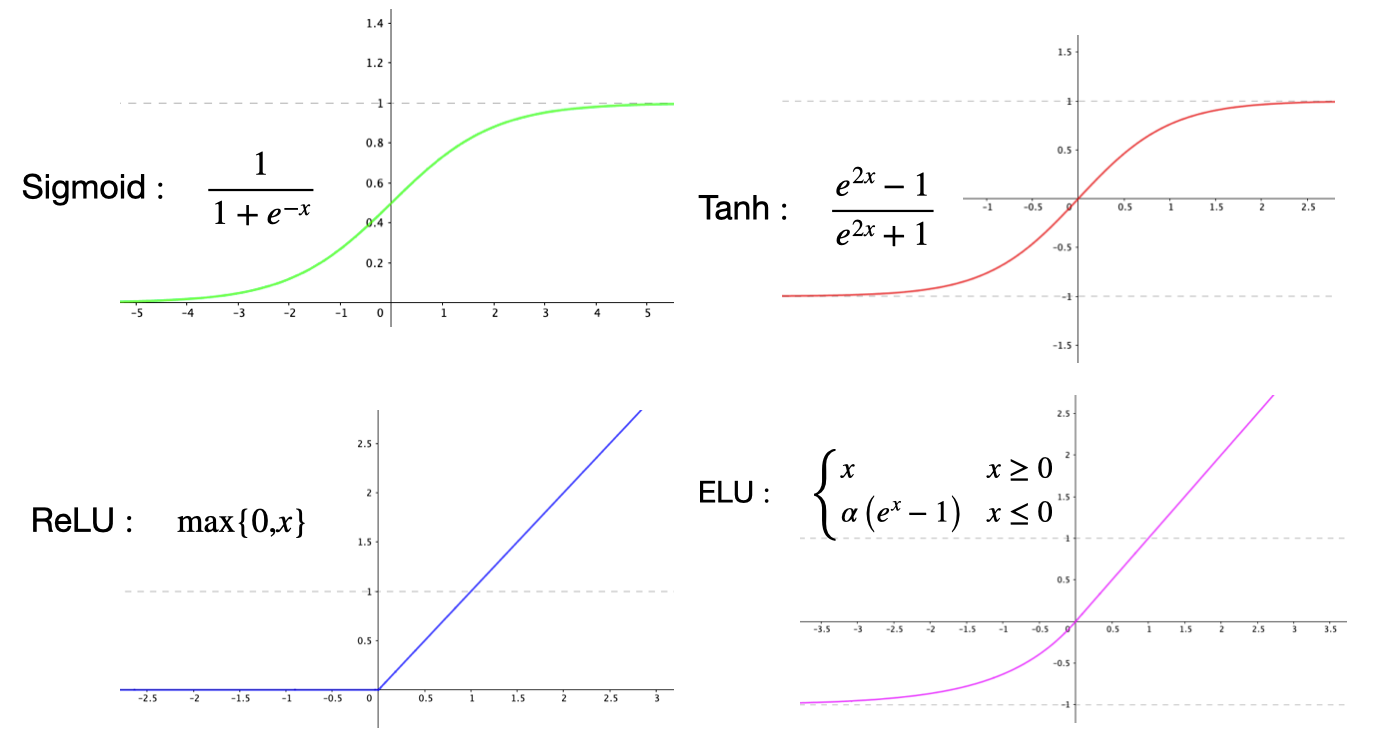
\includegraphics[width=.7\linewidth]{Pics/02_Theory/activation_functions.png}
    \caption{Typical activation functions used in NNs which are all non-linear transforms. The dotted grey lines represent the values of -1 and 1.}
    \label{fig:activation_functions}
\end{figure}

The size and layout of a NN is called the network architecture. The simplest type of NN architecture is the ANN. An example of a very simple ANN with only 2 input values for each observation, and binary output is given in \autoref{fig:very_simple_ANN}. This network has only a single hidden layer with $H$ neurons. 
\begin{figure}
    \centering
    \captionsetup{width=.95\linewidth}
    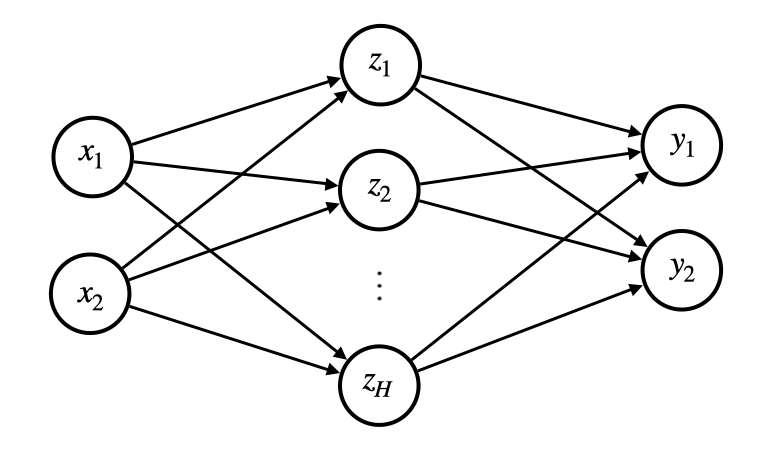
\includegraphics[width=.6\linewidth]{Pics/02_Theory/simple_ANN.png}
    \caption{Illustration of a very simple ANN with only 2 inputs $(x_1, x_2)$, 2 output $(y_1, y_2)$, and a single hidden layer with $H$ neurons $(z_1, z_2,\dots ,z_H)$.}
    \label{fig:very_simple_ANN}
\end{figure}

\subsubsection{Learning}
Learning a NN corresponds to finding the weights of the network that give the highest output accuracy - the best predictions. The method used to find the optimal weights is called back-propagation. This method simply sends inputs through the network and read the outputs. The output error is then propagated backwards through the network in order to adjust the weights accordingly. This is done repeatedly until convergence, normally dividing the training data into smaller batches and performing corrections using every batch. If the amount of data is limited, cross-validation is often used, which trains and validates on the same data. In cross-validation the data is split into a set of folds, and the network is trained on all the data except for one fold which is then used for validating the results.

To represent the error, a so-called loss function is used. Given an observation with input $\bs{x}$ and the corresponding true prediction $y$, we introduce the cost function given by:
\begin{equation}
    L(\Theta | \bs{x},y) = - \hat{p}(y) + \log\left(\sum_{k=0}^K e^{\hat{p}(k)}\right)
\end{equation}
Where $\Theta$ represents all the weights of the network, $K$ is the number of output classes, and $\hat{p}(k)$ is the predicted probability of the input belonging to class $k$. This function is also called the \textit{cross-entropy} loss function and is a the typical choice in classification problems. The cross-entropy loss function can be seen as a function of the weights of the network (here $\Theta$) because the weights are used to find the predictions $\hat{p}$. The gradient of this loss-function with respect to each of the weights in the network is used to update the weights accordingly by a gradient-descent step:
\begin{equation}
    \Theta_{new} = \Theta - \gamma \ \nabla L (\Theta)
\end{equation}
Where $\gamma$ is the learning rate that can be used to determine the speed of the learning, i.e. bigger values implies bigger jumps, while smaller values are used for fine-tuning. This derivative can be found either analytically, by applying the chain rule backwards through the network, or automatically using the \textit{autograd}-function in \textit{PyTorch}. In this thesis the \textit{autograd}-function will be used to find the derivatives, hence for the analytical derivations cf. \cite{elements_NN} or \cite{Zhang2016}.

\subsubsection{Architectures}
NNs are very flexible and can easily be adapted to fit every need. Not only can they be built off an arbitrary number of layers of different sizes, but also there are multiple different types of layers. Each layer finds progressively more complex features in the input data, hence more layers will be able to find more complex features. NNs can be both feed-forward (information flows forward) or recurrent (information flows backwards). The two types of layers that we will cover in this thesis are the dense layer and the convolutional layer respectively. Both have powerful properties and will be discussed further in the following.

\paragraph{The dense layer}
The dense layer is the basic building block of NNs, and ANNs are almost always built of these. A dense layer (also called fully-connected layer) is a layer in which each of neurons have a connection with all the neurons in the previous layer. Both the middle and output layers in the network illustrated in \autoref{fig:very_simple_ANN} are dense layers. In CNNs the dense layers are often used in the last part of the network to condense the information from the convolutional layers.

The dense layer is calculated as the non-linear transform of a matrix-vector product with the matrix consisting of the weights on the edges connecting the layer to the previous, and the vector being the input from the previous layer. This concept is illustrated in \autoref{fig:dense_layer_VM_prod}.
\begin{figure}
    \centering
    \captionsetup{width=.95\linewidth}
    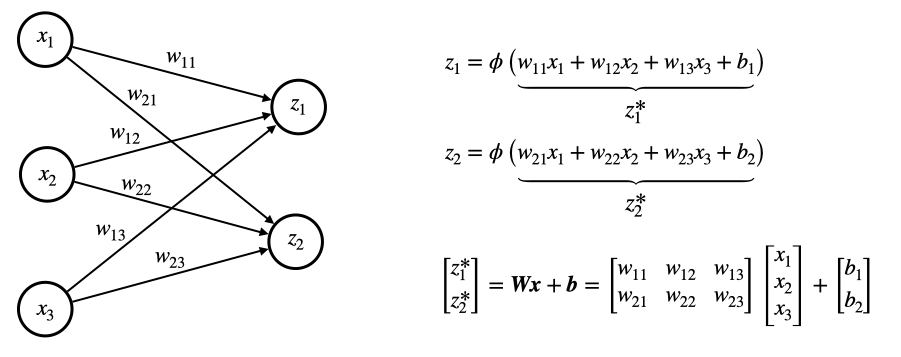
\includegraphics[width=\linewidth]{Pics/02_Theory/dense_layer_VM_prod.png}
    \caption{Illustration of the calculation of the dense layer. $x_i$ and $z_i$ are the $i$th activation of the two layers respectively. $w_{ji}$ is the weight corresponding to the connection between $x_i$ and $z_j$, and $b_i$ is the bias to be added to $z_i$. The dense layer is calculated as the non-linear transform of the bias plus the matrix-vector product between the weight matrix $\bs{W}$ and the input vector $\bs{x}$. $\phi$ is the activation function or non-linear transform.}
    \label{fig:dense_layer_VM_prod}
\end{figure}

\paragraph{The convolutional layer}
The convolutional layer has become a very powerful tool in image classification due to its ability to find features in images using the spatial information. In a convolutional layer the weights are arranged in a number of filters, each of which can be trained to look for specific features. For instance, a low-level filter can search for lines or curves in various directions, while higher-level filters look for e.g. faces, bodies, or wrinkles on clothes \cite{Yosinski2015}. The filters are placed in every position in the input image to calculate the activation at that position simply by multiplying the weights of the filter by the image and summing everything. The resulting activations will also be arranged as an image with high values corresponding to high activations.

Since color-images have multiple input channels (one red, one green, one blue), they are represented as order-3 tensors of size $H \times W \times S$, where $H$ is the image height in number of pixels, $W$ is the width of the image, and $S$ is the number of input channels. The convolution of an input image $\tensor{X}$ with this size into an output tensor $\tensor{Y}$ of size $H' \times W' \times T$ is given by:
\begin{equation}
    \tensor{Y}(h', w', t) =\sum_{i=1}^{D_H} \sum_{j=1}^{D_W} \sum_{s=1}^{S} \ \tensor{K}(i, j, s, t) \ \tensor{X}(h_i, w_j, s)
    \label{eq:2d_convolution_1}
\end{equation}
Where:
\begin{equation}
    h_i =  \left(h' - 1\right) \Delta_H + i - P_H \qquad w_j =  \left(w' - 1\right) \Delta_W + j - P_W
\end{equation}
In \eqref{eq:2d_convolution_1} $\tensor{K}$ is the 4-dimensional kernel of size $D_H \times D_W \times S \times T$ which corresponds to the $T$ different stacked filters of size $D_H \times D_W \times S$. $\Delta$ corresponds to the stride, i.e. how much the filters should move between each calculation (usually 1). $P$ corresponds to the padding which is how many 0s should be put on the edges of the image, and can be used to ensure the same input and output size in terms of the spatial dimensions. $(h_i, w_j)$ is the top left corner of the position in the input image and the three sums correspond to the application of the $t$th filter to that position. The application of a filter to an image with a single input channel is illustrated in \autoref{fig:convolution_illustration}.
\begin{figure}
    \centering
    \captionsetup{width=.95\linewidth}
    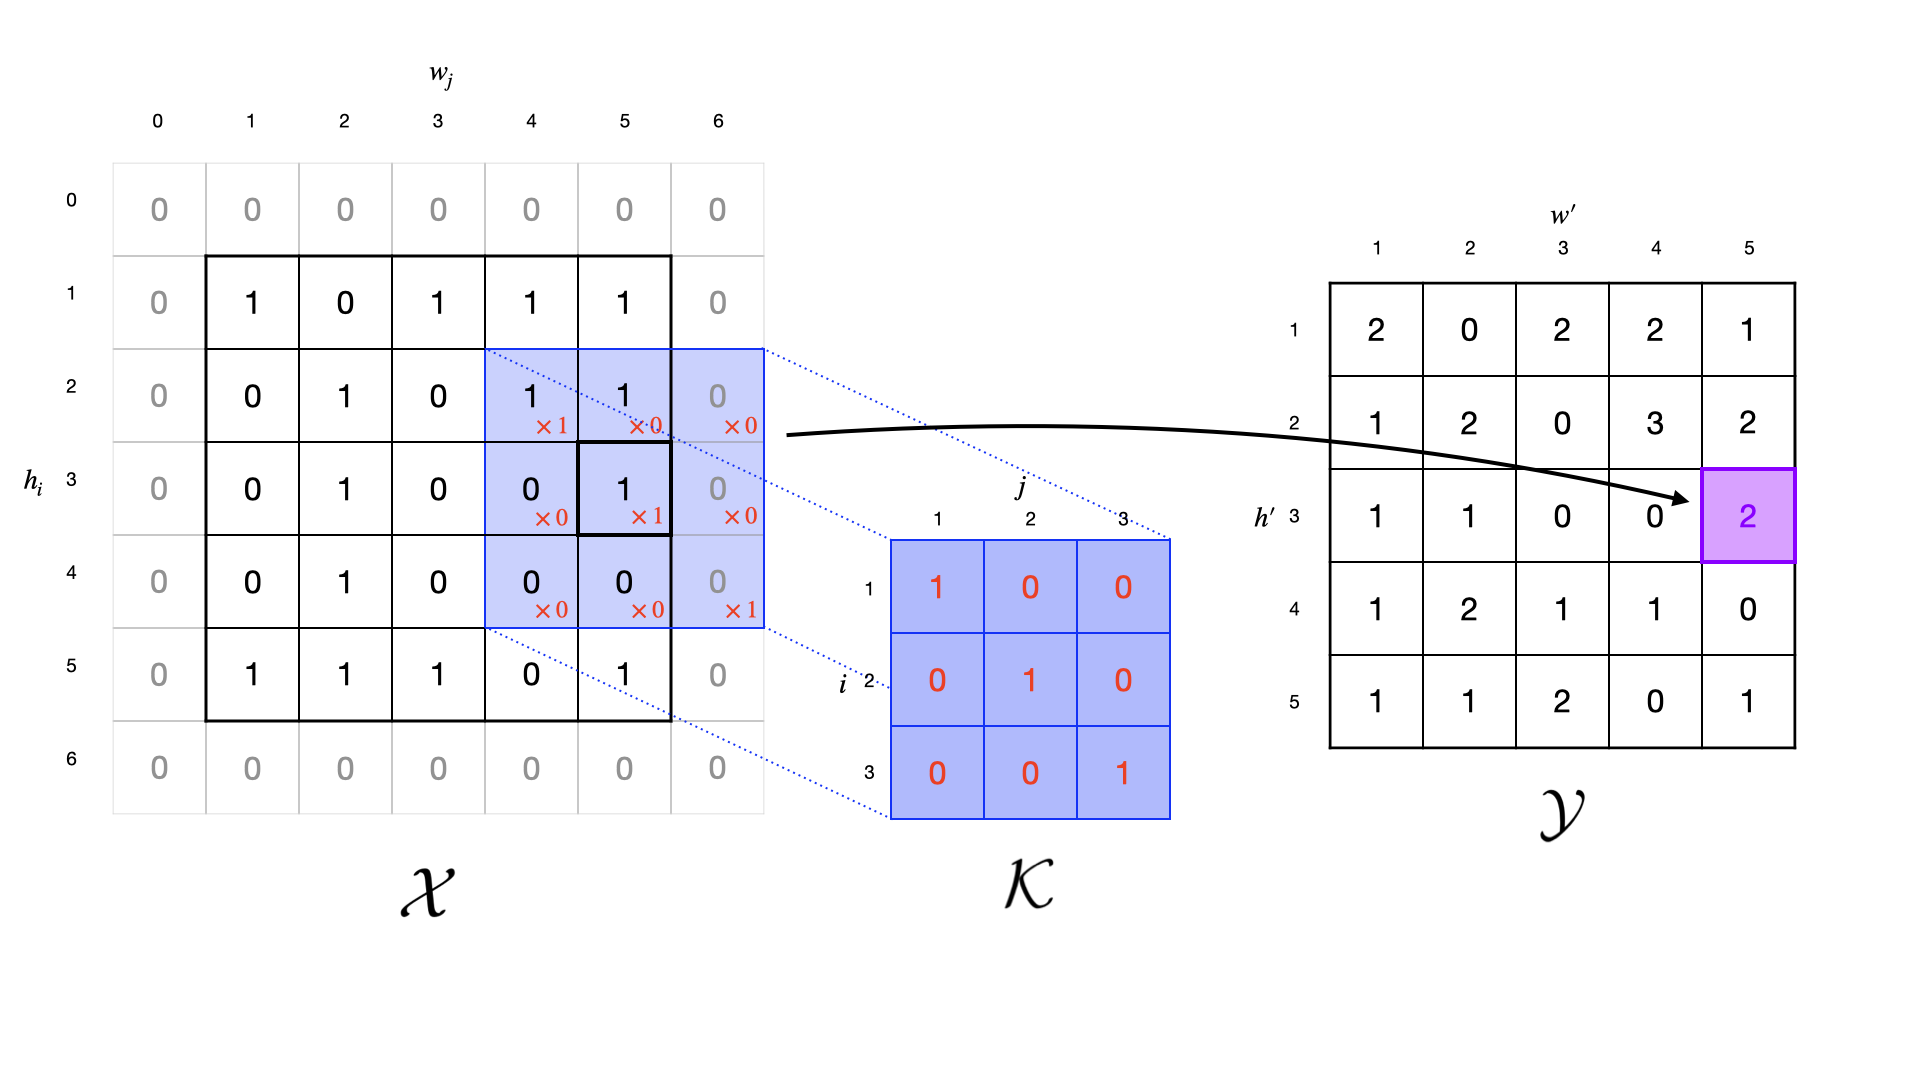
\includegraphics[width=\linewidth]{Pics/02_Theory/convolution_illustration.png}
    \caption{Illustration of a simple convolution of a picture with a single input channel. The calculation of the value $\tensor{Y}(3, 5, \cdot)$ is the one that is highlighted. The arrow signifies the sum of the result of applying the filter $\tensor{K}$ to the input image $\tensor{X}$. The input image will always be 1-indexed, hence the padding (grey 0s) is indexed appropriately. The very simple filter is trained to look for diagonal lines, hence the output will have a high activation if a diagonal line is present in $\tensor{X}$. If there are more input channels, the input image $\tensor{X}$ and the filter $\tensor{K}$ will both be 3-dimensional tensors.}
    \label{fig:convolution_illustration}
\end{figure}
The output size $H' \times W'$ is calculated by the formula:
\begin{align}
    H' &= \frac{H - D_H + 2\cdot P_H}{\Delta_H} + 1 \label{eq:out_dim_H}\\
    W' &= \frac{W - D_W + 2\cdot P_W}{\Delta_W} + 1 \label{eq:out_dim_W}
\end{align}
\subparagraph{The 3D convolution in videos}
There are multiple ways of doing convolutions for videos, that are simply a stack of images. One way is to do convolutions on every frame in a sequence and gathering the result - another way is to apply a 3-dimensional filter.\footnote{This filter will actually be 4-dimensional if there are multiple input dimensions} The 3-dimensional filter will not only look for features in the spatial dimensions, but also for temporal information, i.e. movement. The 3D convolution is very similar to the 2D case \eqref{eq:2d_convolution_1}, except for another sum and higher dimensions. The 3D convolution of an input video $\tensor{X}$ of size $F\times H \times W \times S$ ($F$ is the frames) into an output tensor $\tensor{Y}$ of size $F'\times H' \times W' \times T$ is given by:
\begin{equation}
    \tensor{Y}(f', h', w', t) = \sum_{i=1}^{D_F} \sum_{j=1}^{D_H} \sum_{l=1}^{D_W} \sum_{s=1}^{S} \ \tensor{K}(i, j, l, s, t) \ \tensor{X}(f_i, h_j, w_l, s)
\end{equation}
Where:
\begin{equation}
    f_i = \left(f' - 1\right) \Delta_F + i - P_F \qquad h_j =  \left(h' - 1\right) \Delta_H + j - P_H \qquad w_l =  \left(w' - 1\right) \Delta_W + l - P_W
\end{equation}
Now the convolutional kernel $\tensor{K}$ is 5-dimensional and have the size $D_F \times D_H \times D_W \times S \times T$, which is a stack of 4-dimensional filters. The output size $F'$ is calculated in the same way as \eqref{eq:out_dim_H} and \eqref{eq:out_dim_W} by:
\begin{equation}
    F' = \frac{F - D_F + 2\cdot P_F}{\Delta_F} + 1
    \label{eq:out_dim_F}
\end{equation}

%%%%%%%%%%%%%%%%%%%%%%%%%%%%%%%%%%%%%%%%%%%%%%%%%%%%%%%%%%%%%%%%%%%%%%%%%%%%%%%%%%%
%%%%%  Tensor Decomposition %%%%%%%%%%%%%%%%%%%%%%%%%%%%%%%%%%%%%%%%%%%%%%%%%%%%%%%
%%%%%%%%%%%%%%%%%%%%%%%%%%%%%%%%%%%%%%%%%%%%%%%%%%%%%%%%%%%%%%%%%%%%%%%%%%%%%%%%%%%

\subsection{Tensors and Tensor Decomposition}\label{tex:decomp_methods}
A tensor is a data array of an arbitrary number of dimensions, hence matrices are order-2 tensors, while vectors are order-1 tensors. Tensors are frequently used in many different fields that have to do with computer science\cite{Mørup2011}. Tensors have many great properties due to their many dimensions, but also quickly grow very large.

The concept of tensor decomposition or tensor factorisation concerns itself with exploiting the tendencies of the data in order to find a representation that is smaller and easier to work with. There are multiple representations or decompositions that will be discussed in detail in this section. The Tucker method will be discussed in a bit more detail, due to its importance to the work done in the thesis. Since the python library \textit{TensorLy} has great implementations of the different algorithms, it will be used to calculate the decompositions throughout the thesis. The algorithms for estimating the decomposition are given in \autoref{app:DecompEstimation}.

\paragraph{Basic tensor representation and operations} \label{tex:tensor_operations}
Tensors can be matricized by the use of one of the dimensions

\subsubsection{CP / Parafac}
CP (Candecomp) decomposition that also goes by the names of Parafac or canonical decomposition is the most basic representation. The CP decomposition represents the tensor as the sum of $R$ outer-vector products, where each dimension has a loading vector for each $R$. $R$ is the rank of the decomposition and obviously this allows for more specific details the higher $R$ gets. The CP decomposition of an order-3 tensor $\tensor{X}$ of size $n_1\times n_2 \times n_3$ is given by:
\begin{equation}
    \tensor{X} \approx \sum_{d=1}^R \bs{a}_d \circ \bs{b}_d \circ \bs{c}_d
\end{equation}
Or element-wise:
\begin{equation}
    \tensor{X}(i, j, l) \approx \sum_{d=1}^R \bs{a}_d(i) \cdot \bs{b}_d(j) \cdot \bs{c}_d(l)
\end{equation}
Where $\boldsymbol{a}_i$, $\boldsymbol{b}_i$, and $\boldsymbol{c}_i$ are the $i$th loading vectors of each dimension respectively. If each of these loading vectors are concatenated to form loading matrices, the decomposition can also be written in the following way using a diagonal or identity tensor $\tensor{D}$ and $n$-mode products:
\begin{equation}
    \tensor{X}^{n_1 \times n_2 \times n_3} \approx \tensor{D}^{R\times R\times R} \times_1 \bs{A}^{n_1 \times R} \times_2 \bs{B}^{n_2 \times R} \times_3 \bs{C}^{n_3 \times R}
    \label{eq:CP_matrix_rep}
\end{equation}
$\tensor{D}$ is also called the core tensor. For the loading matrices we have that:
\begin{equation}
    \bs{A} = \begin{bmatrix} | & | & & |\\ \bs{a}_1 & \bs{a}_2 & \dots & \bs{a}_R \\ | & | & & | \end{bmatrix} \qquad \bs{B} = \begin{bmatrix} | & | & & |\\ \bs{b}_1 & \bs{b}_2 & \dots & \bs{b}_R \\ | & | & & | \end{bmatrix} \qquad \bs{C} = \begin{bmatrix} | & | & & |\\ \bs{c}_1 & \bs{c}_2 & \dots & \bs{c}_R \\ | & | & & | \end{bmatrix}
\end{equation}
The CP decomposition is illustrated in \autoref{fig:CP_decomp_illustration}.
\begin{figure}
    \centering
    \captionsetup{width=.95\linewidth}
    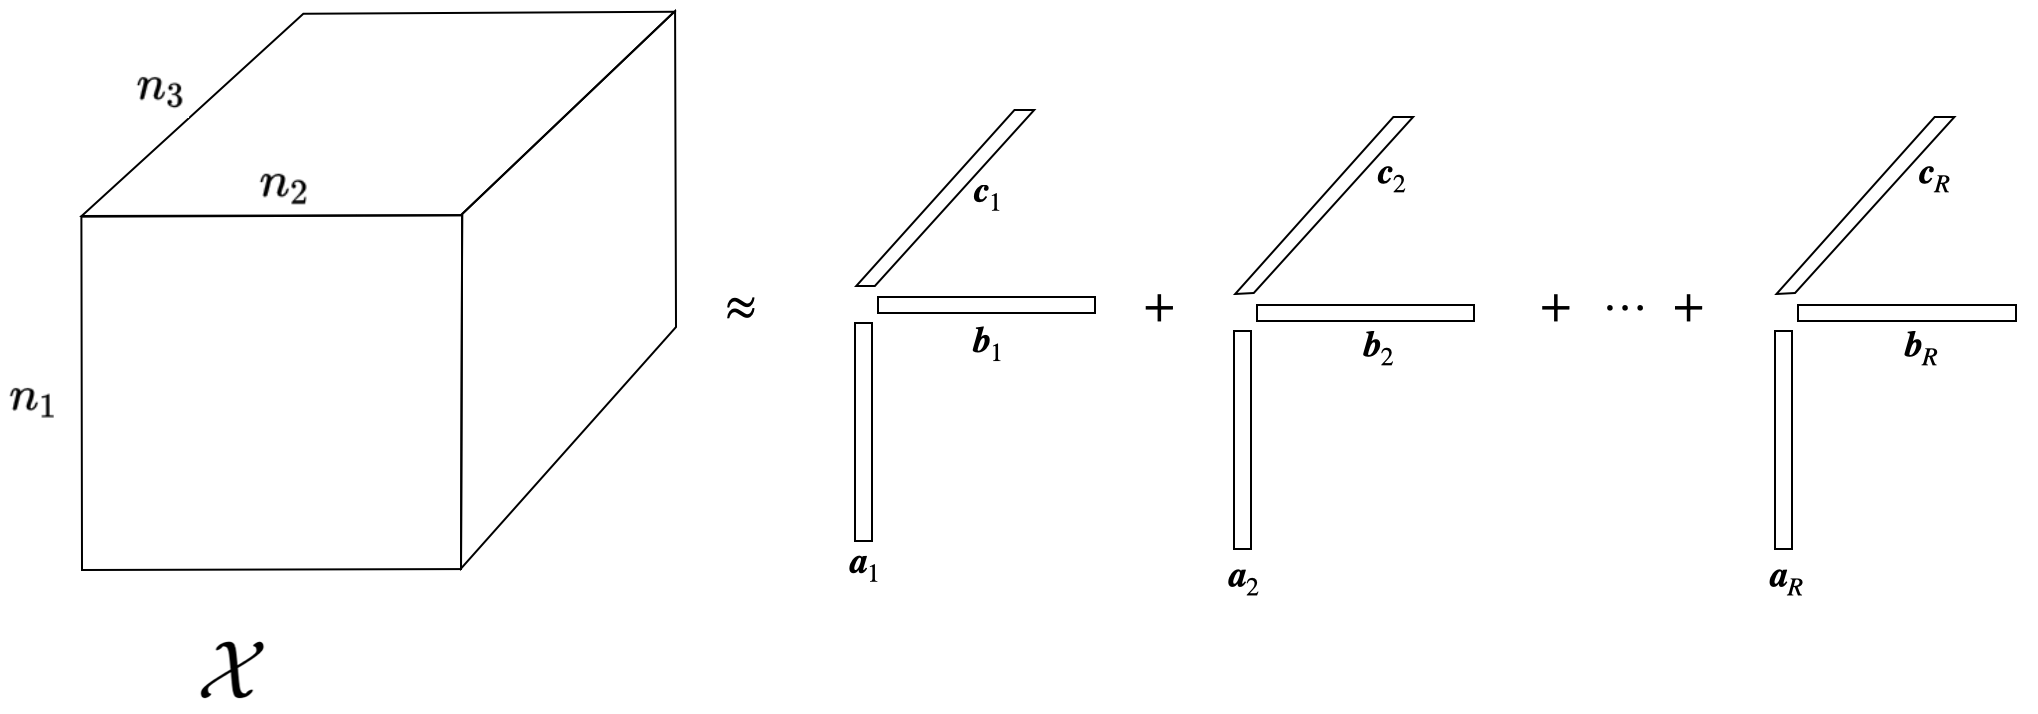
\includegraphics[width=\linewidth]{Pics/02_Theory/CP_decomp_illustration.png}
    \caption{The tensor $\tensor{X}$ is decomposed using the CP decomposition. The CP decomposition approximation is the sum of a sequence of $R$ outer-vector products, with $R$ being the rank of the decomposition. The vectors have length corresponding to the length of the dimension in $\tensor{X}$, e.g. all the $\bs{a}$-vectors have length $n_1$.}
    \label{fig:CP_decomp_illustration}
\end{figure}

Due to the nature of the CP decomposition only the $i$th loading of each loading vector can interact with each other, making the CP decomposition rather restricted. However the restriction of this representation implies a unique optimal solution of the CP decomposition, which desirable. The method is good at resolving different additive physical profiles, e.g. if addition of multiple chemicals to a solution have different effects on a response variable, these can be resolved. CP decomposition however fails when different dimensions are correlated, due to strong cancellation effects between the various components of the representation, making it slow to converge and hard to interpret \cite{Mørup2011}.

\subsubsection{Tucker}
Tucker decomposition is the less restricted version of the CP decomposition - or actually CP decomposition is a special case of Tucker. In Tucker decomposition loadings can interact with each other even crisscrossing, which gives this representation a good deal of freedom. This is achieved allowing the core-tensor $\tensor{D}$ ($\tensor{G}$ for Tucker) to be non-diagonal, hence we also get to choose special ranks for each dimension. Thus the Tucker decomposition is a sum of outer-vector products scaled by the core element. Based on the matrix-representation of the CP decomposition \eqref{eq:CP_matrix_rep}, the Tucker decomposition of an order-3 tensor $\tensor{X}$ of size $n_1 \times n_2 \times n_3$ is given as:
\begin{equation}
    \tensor{X}^{n_1 \times n_2 \times n_3} \approx \tensor{G}^{R_A \times R_B \times R_C} \times_1 \bs{A}^{n_1 \times R_A} \times_2 \bs{B}^{n_2 \times R_B} \times_3 \bs{C}^{n_3 \times R_C}
\end{equation}
Where $\bs{A}$, $\bs{B}$, and $\bs{C}$ are the loading matrices of each of the dimensions and $R_A$, $R_B$, and $R_C$ are the ranks of the decomposition in each of the dimensions. $\tensor{G}$ is the core tensor that we in the Tucker case allow to be non-diagonal. We can also write the Tucker representation element-wise:
\begin{equation}
    \tensor{X}(x_1,x_2,x_3) \approx \sum_{r_A=1}^{R_A} \sum_{r_B=1}^{R_B} \sum_{r_C=1}^{R_C} \tensor{G}(r_A, r_B, r_C) \cdot \bs{A}(x_1, r_A) \cdot \bs{B}(x_2, r_B) \cdot \bs{C}(x_3, r_C)
\end{equation}
The concept of Tucker decomposition is shown in \autoref{fig:tucker_decomp_illustration}. 
\begin{figure}
    \centering
    \captionsetup{width=.95\linewidth}
    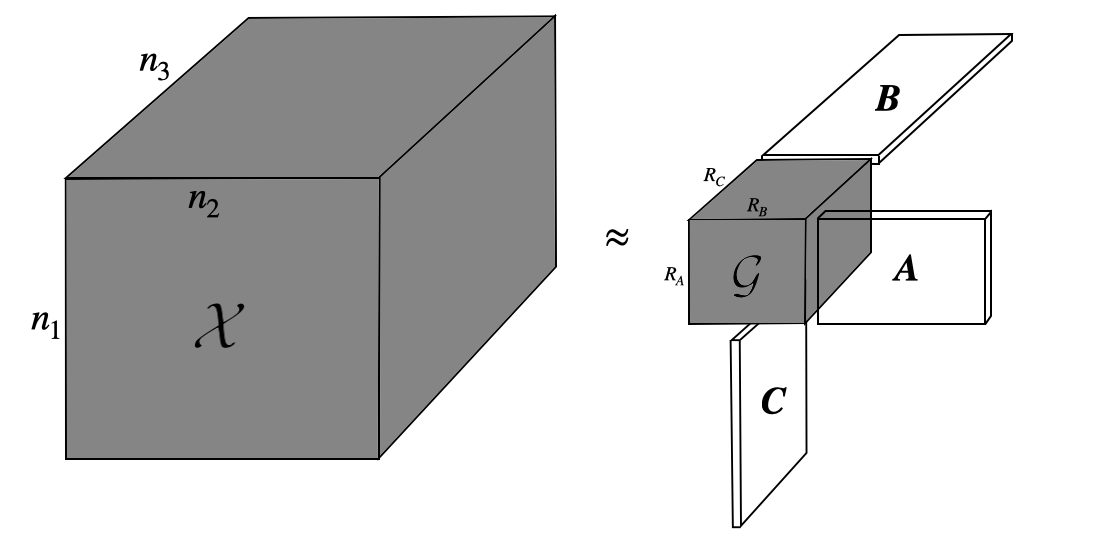
\includegraphics[width=.7\linewidth]{Pics/02_Theory/Tucker_decomp_illustration.png}
    \caption{The tensor $\tensor{X}$ is decomposed using Tucker-3 decomposition, which means that all 3 dimensions will be decomposed. The Tucker decomposition is a sequence of $n$-mode products between the core tensor $\tensor{G}$ and the three loading matrices $\bs{A}$, $\bs{B}$, and $\bs{C}$. The size of $\tensor{G}$ is equal to the ranks of the decomposition, i.e. $R_A \times R_B \times R_C$. The length of the first dimension of the loading matrices correspond to the length of the given dimension, e.g. for $\bs{A}$ it is $n_1$}
    \label{fig:tucker_decomp_illustration}
\end{figure}
The different rank along each of the dimensions, makes the user able to choose how many different features the algorithm should find along each dimensions. The flexibility of the Tucker decomposition makes it useful for many applications, one of them being the data compression task. The flexibility however also comes at a cost; the representation does not yield unique optimal solutions, and the results harder to interpret than for CP decomposition.

Rank selection for the Tucker decomposition is either choosing appropriate ranks for the problem, or to find the minimal set of ranks $(R_A, R_B, R_C)$ that ensure that:
\begin{equation}
    \tensor{X} = \sum_{r_A=1}^{R_A} \sum_{r_B=1}^{R_B}
 \sum_{r_B=1}^{R_B} \tensor{G}(r_A, r_B, r_C) \cdot \bs{a}_{r_A} \circ \bs{b}_{r_B} \circ \bs{c}_{r_C}
 \end{equation}
I.e. the approximation being equal to the actual tensor. Here $\bs{a}_i$, $\bs{b}_i$, and $\bs{c}_i$ are the $i$th column of the loading matrices respectively. Finding the optimal ranks is a challenging problem, which have been solved in different ways. Due to the challenge of the problem, this thesis will make use of the analytical solution to variational Bayesian matrix factorization (VBMF) by inspiration from Kim et. al \cite{Kim2016}. This approach is chosen because it is a good and easily reproducible heuristic, even though it is sub-optimal. VBMF will be discussed in the following.

\paragraph{Variational Bayesian Matrix Factorization}
The global analytical solution to the VBMF have been derived by Nakajima et. al in 2013 \cite{Nakajima2013}, and can be used as a method for rank selection for the Tucker model\footnote{Also applicable to CP-decomposition, since it is a special case of Tucker decomposition}. The authors use a probabilistic model to find the optimal low-rank factorization of a matrix, automatically taking care of the noise. Given an matrix $\bs{V}$ of size $L\times M$ that is assumed to be the sum of a target matrix and an error matrix:
\begin{equation}
    \bs{V}^{L\times M} = \bs{U}^{L\times M} + \bs{E}^{L\times M}
\end{equation}
The goal is to find matrices $\bs{A}$ and $\bs{B}$ such that:
\begin{equation}
    \bs{U} = \bs{B}\bs{A}^{\top}
\end{equation}
This is achieved by considering a probabilistic model of $\bs{V}$ given prior variances, and use this model to compute the posterior distributions of $\bs{V}$, $\bs{A}$, and $\bs{B}$. Doing this is generally a non-convex problem why the analytical solution is key. This however does only work for matrices, hence tensors of order $> 2$ need to be converted into matrices using matricization discussed in \autoref{tex:tensor_operations}. Matricization using the $i$th dimension gives the estimated rank of that same dimension of the tensor. It should be noted that this method only works when the $L < M$, since we need to have $\frac{L}{M} < 1$ to satisfy the nature of the probabilistic distribution.

\subsubsection{Block-Term Decomposition}
Block-Term Decomposition (BTD) is simply a sum of Tucker terms, i.e. given an order-3 tensor $\tensor{X}$ and a rank $R$ the BTD of $\tensor{X}$ is given by:
\begin{equation}
    \tensor{X} = \sum_{r=1}^R \tensor{G}_r \times_1 \bs{A}_r \times_2 \bs{B}_r \times_3 \bs{C}_r
\end{equation}
Where we now have $R$ sets of a core and loading matrices instead of a single one of each, which also means that the ranks of the individual Tucker terms can differ to comply with various needs.

\subsubsection{Tensor-Train decomposition}
Tensor-Train (TT) decomposition that also goes by the name "matrix product state decomposition", was developed by Oseledets in 2011, as a simple and non-recursive tensor decomposition representation.\cite{Oseledets2011} TT-decomposition does not make use of a core tensor, but allows for all the loadings arrays to be order-3 tensors. Given an order-$d$ tensor $\tensor{X}$ of size $n_1\times n_2 \times \dots \times n_d$, we will have a sequence of ranks $r_0, r_1, \dots, r_d$, with boundary conditions $r_0=r_d=1$. The TT-decomposition of $\tensor{X}$ is given by:
\begin{equation}
    \tensor{X}(i_1, i_2, \dots, i_d) \approx \tensor{G}_1[i_1] \tensor{G}_2[i_2] \cdots \tensor{G}_d[i_d]
\end{equation}
Where $\tensor{G}_i$ is the $i$th loading tensor of size $r_{i-1}\times n_1\times r_i$, and $\tensor{G}_i[j]$ is the $j$th lateral slice of $\tensor{G}$, which makes it a matrix of size $r_{i-1}\times r_i$. The calculation of a single value at position $(i_1, i_2, \dots, i_d)$ is illustrated in \autoref{fig:TT_decomp_illustration}.
\begin{figure}
    \centering
    \captionsetup{width=.95\linewidth}
    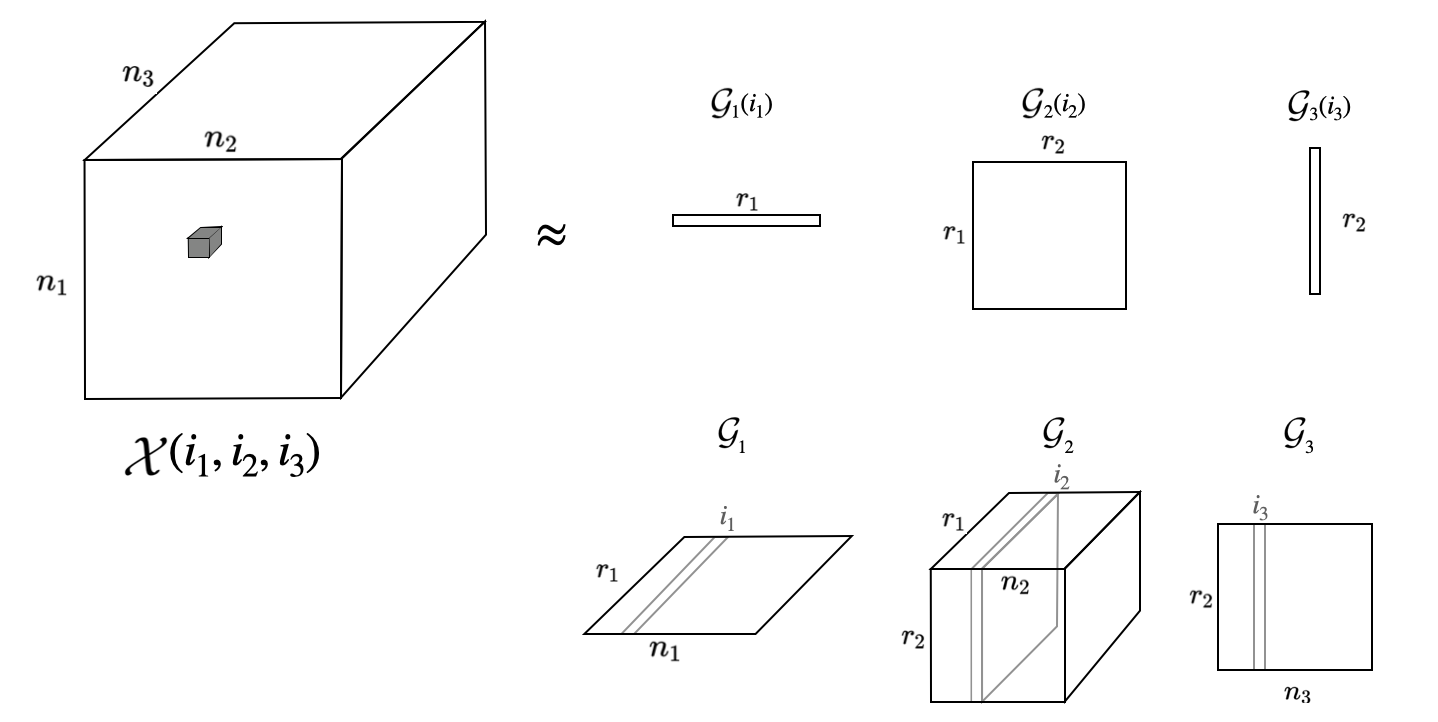
\includegraphics[width=.9\linewidth]{Pics/02_Theory/TT_decomp_illustration.png}
    \caption{The approximation of a single value of the target tensor using the TT-decomposition. The value is the result of a vector-matrix-vector product between $\tensor{G}_1(i_1)$, $\tensor{G}_2(i_2)$, and $\tensor{G}_3(i_4)$ that are slices of the loading tensors $\tensor{G}$. The bottom row shows how the vectors and the matrix are taken out of the $\tensor{G}$s using the given indices $i_1$, $i_2$, and $i_3$.}
    \label{fig:TT_decomp_illustration}
\end{figure}

The TT-decomposition is not prone to the curse of dimensionality, it is stable, and has asymptotically the same number of parameters as CP-decomposition. Oseledets have in \cite{Oseledets2011} also derived efficient versions of basic tensor operations in the TT-format.
\clearpage

%\section{Previous Work} \label{tex:previous_work}
In this section a recap of some different approaches to speed up or decrease the number of parameters will be given. In 2013 Denil et al. found NNs to be heavily over-parametrized \cite{Denil2013}. They did this by training only a fraction of the weights and using these to predict the rest of the weights. They reported that in some cases more than 95\% of the weights could be predicted, hence would not need to be learned. Ever since, numerous attempts have been proposed to optimise the evaluation time and number of parameters in NNs. One approach have been to decompose the dense layer of a NN, an other have tried speeding up the evaluation of a convolution, and some have had success in decomposing and speeding up an entire network. All the work described below follow approximately the same structure:

\begin{enumerate}
    \item \textbf{Decompose weights of pre-trained NN} using some specific algorithm to get a smaller representation of the weights or filters
    \item \textbf{Changing the evaluation algorithm} in order for it to correspond to original evaluations and in order to do back-propagation
    \item \textbf{Fine-tuning} which is training the network using the new algorithm and back-propagation 
\end{enumerate}
Some approaches will be discussed in the following. In the end the methods will be compared in terms of performance in relation to the number of parameters and the computation time.

\subsection{Decomposing the dense layer}
In 2015 Nokinov et al. used TT-decomposition to decompose the weights of a dense (fully-connected) layer in an ANN\cite{Novikov2015}. This method exploits the power of the dense layer and allows it to have a big amount of neurons. The dense layer performs a linear transformation on an input vector $\bs{x}$ of dimension $N$:
\begin{equation}
    \bs{y} = \bs{W} \bs{x} + \bs{b}
    \label{eq:linearTransform}
\end{equation}
Where $\bs{W} \in \R^{M\times N}$ is the weight matrix and $\bs{b} \in \R^{M}$ is the bias vector. $M$ is the dimension of the output $\bs{y}$. Since the weights of the dense layer are given in a matrix, Nokinov et al. folds this matrix into a 3-dimensional tensor in order to decompose it using the TT algorithm. They define the TT-layer to be the same transformation but with the weights stored in the TT-format. Let $\tensor{X}$ be the input tensor of dimension $d$ (formed from $\bs{x}$), and let the decomposition of the weight matrix have cores $\bs{G}_k[i_k, j_k]$. In the TT-layer the transformation corresponding to \eqref{eq:linearTransform} is given as:
\begin{equation}
    \tensor{Y}(i_1, i_2, \dots, i_d) = \sum_{j_1, j_2, \dots, j_d} \bs{G}_1[i_1, j_1] \bs{G}_2[i_2, j_2]\dots \bs{G}_d[i_d, j_d] \tensor{X}(j_1, j_2, \dots j_d) + \tensor{B}(i_1, i_2, \dots, i_d)
\end{equation}
Where $\tensor{B}$ is the bias tensor. The properties of the TT-format allows for computation of back-propagation, which is then used for fine-tuning the network. The authors report a best-case compression of a dense layer of up to 200,000 times and of a whole network of up to 7.

\subsection{Speeding up the evaluation of a convolution}
In 2013 Rigamonti et al. \cite{Rigamonti2013} found that filters can be computed as a linear combination of smaller separable filters. A filter is called separable when it can be expressed using multiple parts of lower dimension, as for instance using the CP-decomposition as illustrated by \cite{Sironi2015} in \autoref{fig:separable_filters}. Ever since many approaches have been considered using this principle in different ways. For instance Jaderberg et al. proposed two different schemes for using rank-1 filters to exploit the cross-channel / filter redundancy \cite{Jaderberg2014}. Since these schemes did not built upon any decomposition algorithm per se, the approximation of the separated filters was done by numerically minimizing either the $L_2$ reconstruction error or the reconstruction error of the output of the given layer (indirectly). Two other approaches uses standard decomposition algorithms to ease the evaluation time. One was proposed by Lebedev et al. in 2015 and used CP-decomposition to decompose the convolutional kernel \cite{Lebedev2015}, another was proposed by Wang and Cheng in 2016 and used BTD. They will both be discussed in the following.

\begin{figure}
    \centering
    \captionsetup{width=.9\linewidth}
    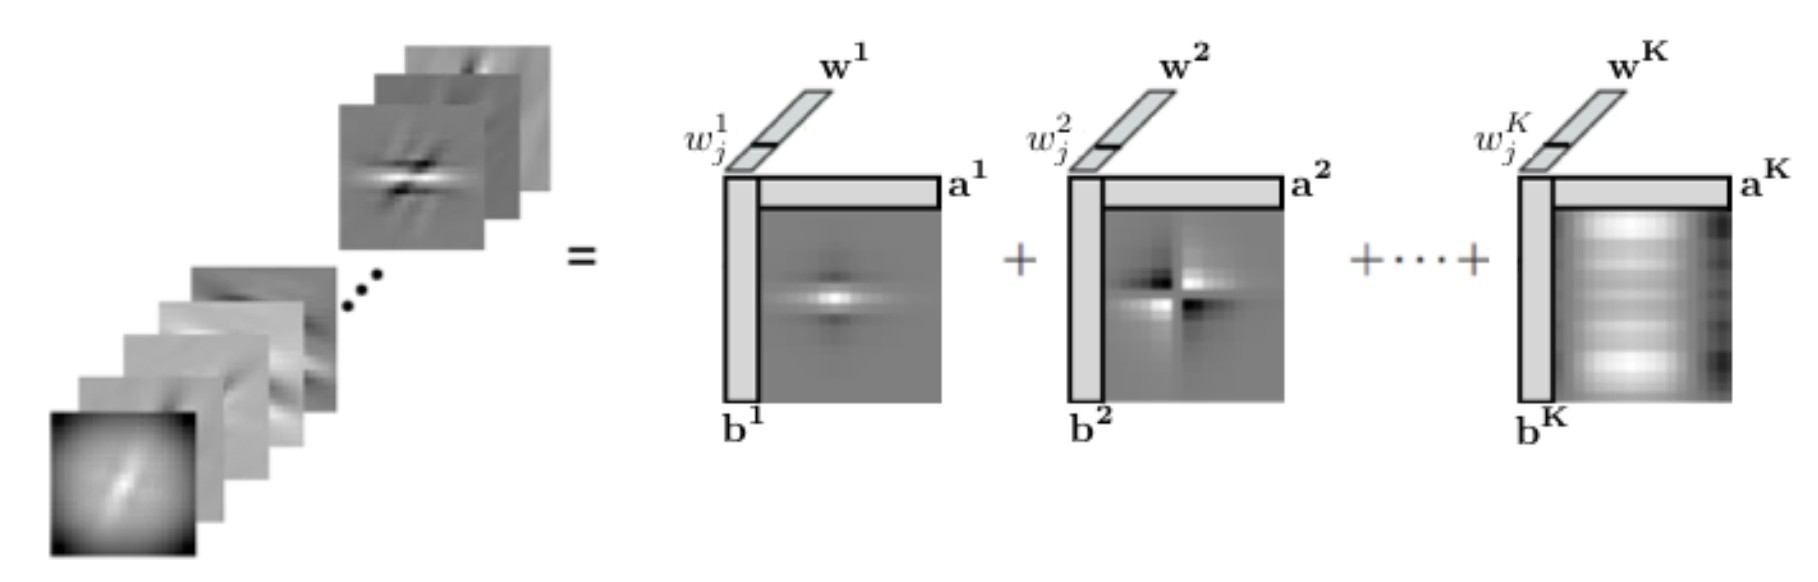
\includegraphics[width=.8\linewidth]{Pics/03_Previous_work/separable_filters.png}
    \caption{Taken from \cite{Sironi2015}. Left: A bank of two-dimensional filters is stacked together to form a 3-dimensional tensor. Right: The tensor is decomposed in the sum of $K$ rank-one tensors. Thus, the original filters are approximated by the weighted sum of the separable filters $s_k = \boldsymbol{a}_k \circ \boldsymbol{b}_k$}
    \label{fig:separable_filters}
\end{figure}

\subsubsection{Convolution using CP-decomposition} \label{tex:convUsingCP}

Lebedev et al. proposed to decompose the 4-dimensional convolutional kernel using CP\Hyphdash decomposition \cite{Lebedev2015}. The idea is to reduce the computation time of the evaluation of a convolutional layer. After having decomposed the kernel into a set of rank-1 tensors, they re-write the convolution into an expression of nested sums using the loadings of the decomposition. The traditional convolution of an input tensor $\tensor{U}$ of size $W \times H \times S$ into an output tensor $\tensor{T}$ of size $(W-d+1)\times (H-d+1)\times t$ looks like this:
\begin{equation}
    \tensor{V}(x, y, t)=\sum_{i=x-\delta}^{x+\delta} \sum_{j=y-\delta}^{y+\delta} \sum_{s=1}^{S} \tensor{K}(i-x+\delta, j-y+\delta, s, t) \ \tensor{U}(i, j, s)
    \label{eq:tradConvolution}
\end{equation}
Where $\tensor{K}$ is the 4-dimensional kernel\footnote{The kernel corresponds to a stack of 3-dimensional filters} of size $d\times d \times s\times t$ and $\delta = \frac{d-1}{2}$ is the half width of the filter in the spatial dimension. Using the decomposition of $\tensor{K}$ with loading matrices $\bs{K}_w$, $\bs{K}_h$, $\bs{K}_s$, and $\bs{K}_t$, the (approximated) convolution \eqref{eq:tradConvolution} can be written as:
\begin{equation}
    \tensor{V}(x, y, t) = \sum_{r=1}^{R} \bs{K}_{t}(t, r)\left(\sum_{i=x-\delta}^{x+\delta} \bs{K}_{w}(i-x+\delta, r)\left(\sum_{j=y-\delta}^{y+\delta} \bs{K}_{h}(j-y+\delta, r)\left(\sum_{s=1}^{S} \bs{K}_{s}(s, r) \ \tensor{U}(i, j, s)\right)\right)\right)
\end{equation}
With $R$ being the rank of the decomposition. Now each of the parenthesis can be expressed as intermediate tensors, which means that the whole convolution can be broken into a sequence of four simple convolutions. \autoref{fig:decompConvDifference} shows the difference between a traditional convolution and the sequence of convolutions using the decomposition. The expression of the convolution using the decomposed kernel allows as a sequence of simpler convolutions allows for the use of standard back-propagation. Furthermore it enables easy fine-tuning of the entire network. The authors report that even though the reconstruction error decreases with the increasing rank, a high accuracy is not needed in order to get good prediction results. They also state that their method works well for smaller architectures, while it has a harder time on more complex ones.

\begin{figure}
    \centering
    \begin{subfigure}{\linewidth}
        \centering
        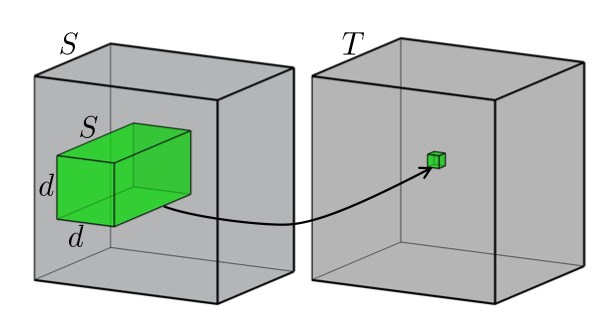
\includegraphics[width=0.4\linewidth]{Pics/03_Previous_work/fullConv.png}
        \caption{Original convolution}
    \end{subfigure}
    \begin{subfigure}{\linewidth}
        \centering
        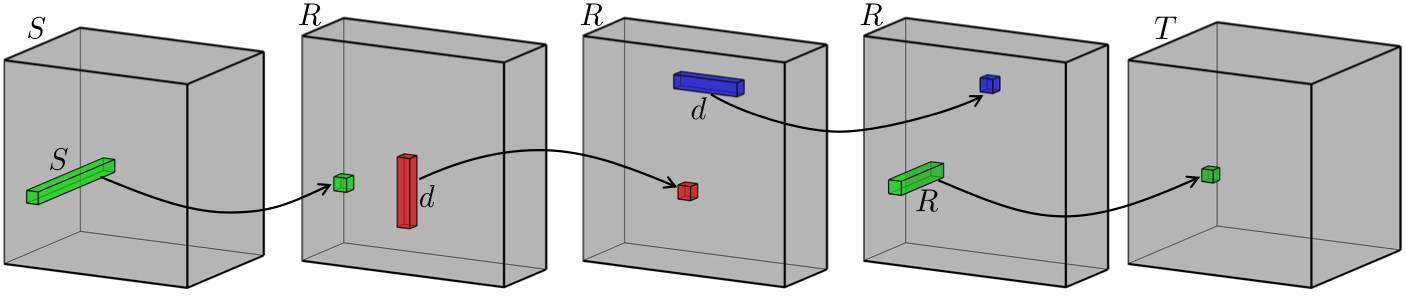
\includegraphics[width=\linewidth]{Pics/03_Previous_work/decompConv.png}
        \caption{Convolution using CP-decomposed kernel}
    \end{subfigure}
    \captionsetup{width=.95\linewidth}
    \caption{Taken from \cite{Lebedev2015}. The difference between the original convolution and the sequence of convolutions using the loadings vectors of the CP-decomposition. The grey boxes corresponds to the 3-dimensional tensors within the CNN, with the frontal sides corresponding to the spatial dimension. For instance the first box in each line corresponds to the input image where $S$ is the number of input channels. The arrows show linear mappings, or how to calculate a single value using a filter (top) or a decomposed filter (bottom).}
    \label{fig:decompConvDifference}
\end{figure}

\subsubsection{Convolution using Block Term Decomposition}
Wang and Cheng proposed speeding up the evaluation of a convolution using BTD, which benefits from both sparsity and low-rank. For simplicity they combine the two spatial dimensions into one which means that the convolutional kernel becomes 3-dimensional ($S\times T \times WH$). Since they will not exploit the spatial dimension due to low rank, their decomposition becomes a tucker-2 decomposition of the kernel $\tensor{K}$:
\begin{equation}
    \tensor{K} \approx \sum_{r=1}^{R} \tensor{G}_r \times_1 \bs{A}_r \times_2 \bs{B}_r
\end{equation}
Where $R$ is the rank of the BTD, $\bs{A}_r \in \R^{S\times s}$ and $\bs{B}_r \in \R^{T\times t}$ are the factor matrices along input and output channel dimensions respectively. $\tensor{G}_r \in \R^{s\times t \times P}$ is the core of the $r$'th subtensor. Now the authors concatenate all the $R$ matrices into big matrices $\bs{A}$ and $\bs{B}$. And the core tensors into a big group-sparse core matrix $\tensor{G}$. The result is visualized in \autoref{fig:concatBTD}. The convolution can be done faster using this decomposition and the sequence of convolutions shown in \autoref{fig:BTD_conv_decomp}. The authors also propose a new algorithm for doing the decomposition itself. They call the algorithm Principle Component Iteration (PCI) which is a generalisation of higher order orthogonal iteration (HOOI)

\begin{figure}
    \centering
    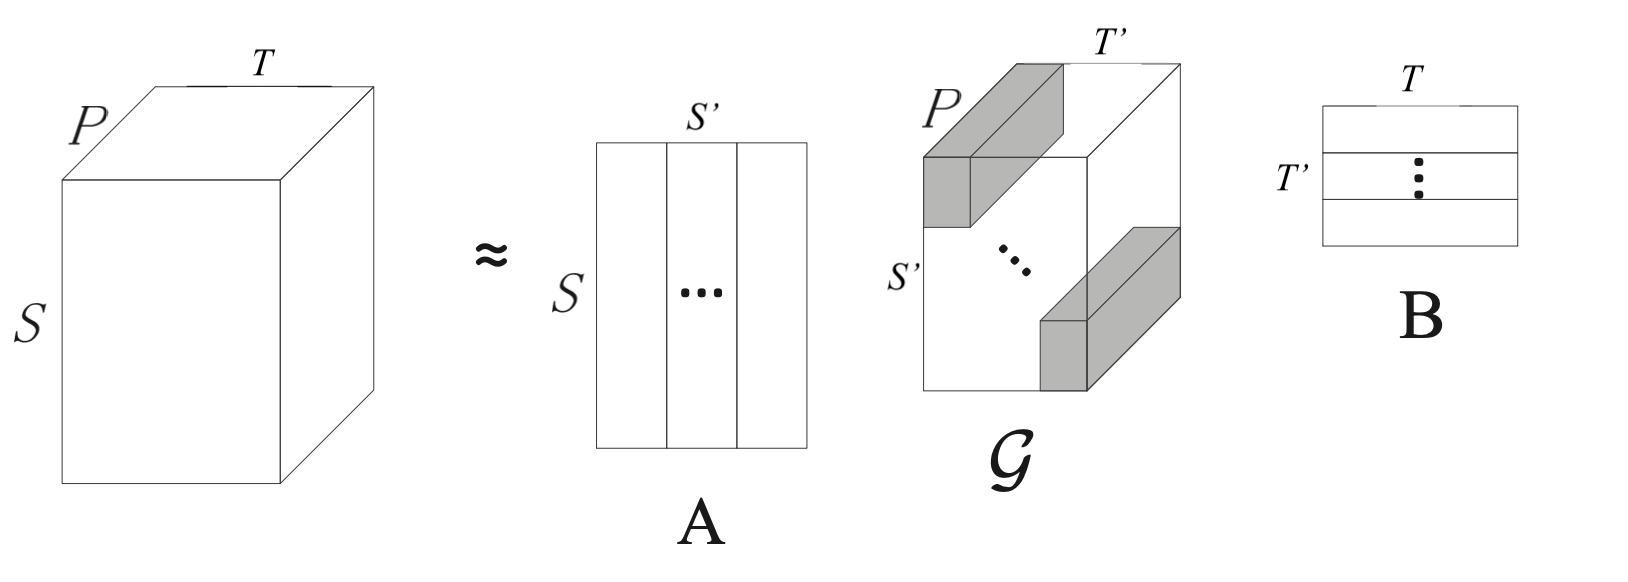
\includegraphics[width=0.8\linewidth]{Pics/03_Previous_work/concatBTD.png}
    \captionsetup{width=.85\linewidth}
    \caption{Taken from \cite{Wang2016}. Illustrates how the $R$ factor matrices and core tensors can be concatenated.} 
    \label{fig:concatBTD}
\end{figure}

\begin{figure}
    \centering
    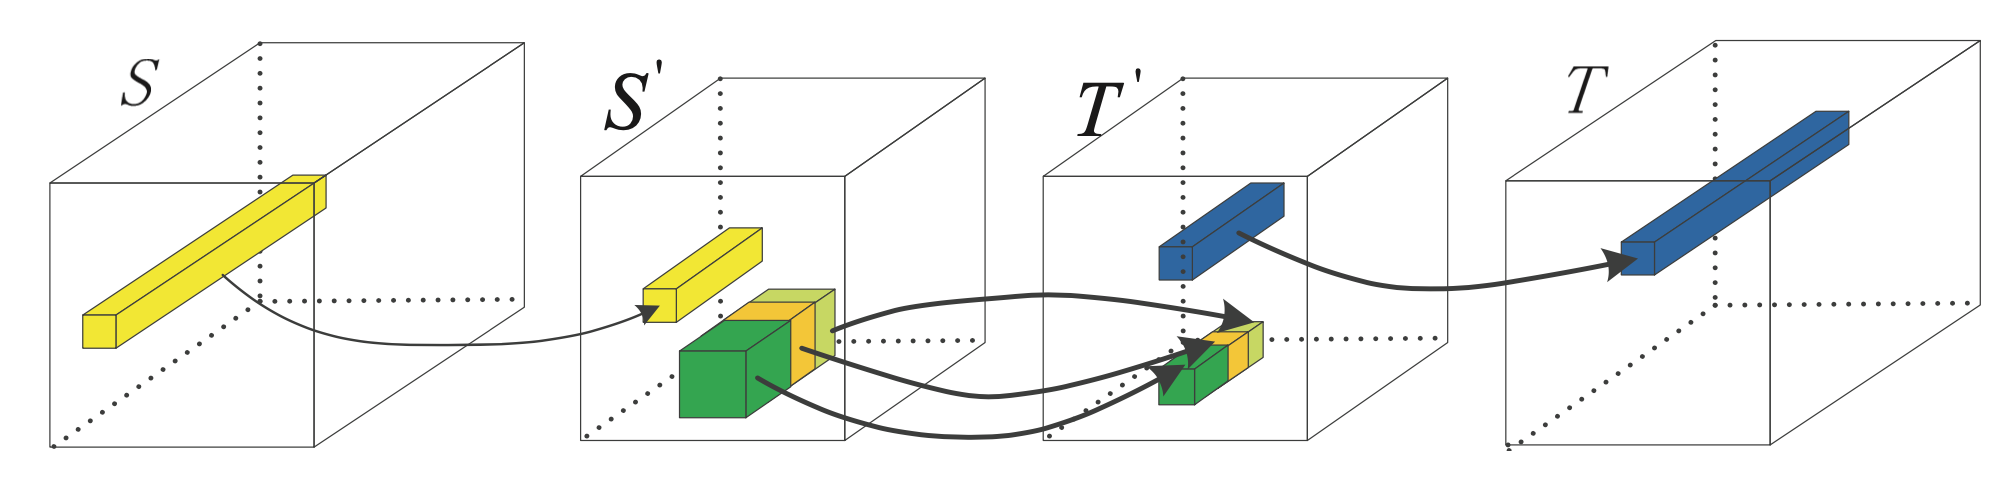
\includegraphics[width=.8\linewidth]{Pics/03_Previous_work/BTD_conv_decomp.png}
    \captionsetup{width=.85\linewidth}
    \caption{Taken from \cite{Wang2016}. Illustrates how the convolution is done using the BTD. Each of the boxes correspond to an intermediate tensor with the frontal sides corresponding to spatial dimensions. The arrows show a linear mapping using the factors of the filter.}
    \label{fig:BTD_conv_decomp}
\end{figure}

\subsection{Speeding up the entire network} \label{tex:sub_entire_network}
All the methods discussed above only describe how to decompose a single layer in the NN; the dense layer or the convolutional layer respectively. In 2016 one method was proposed that would be able to decompose an entire network at once.

Kim et al. proposed using Tucker-decomposition to decompose, not only the convolutional layers, but also the dense layers \cite{Kim2016}. They would use Tucker-2 decomposition from the second convolution to the first dense layer, and Tucker-1 decomposition\footnote{Equivalent to the SVD} for the remaining. They did not decompose the spatial dimensions, since these already are quite small. They also proposed using the global analytical solutions for variational Bayesian matrix factorization (VBMF) developed by Nakajima et al. in 2013 \cite{Nakajima2013} to find the optimal ranks for the decompositions. In a similar derivation to the one in \autoref{tex:convUsingCP}, Kim et al. found that the Tucker-2 decomposed convolutional layer can be described as a sequences of simpler convolutions. This sequence is shown in \autoref{fig:tuckerDecompConv}. They use this sequence to do back-propagation on the entire network at once. The authors report promising results, but states that the optimality of the rank selection needs to be investigated further. They also claim that the $1\times 1$ convolution has great potential and will grow in popularity.\footnote{The yellow and blue convolutions seen in \autoref{fig:tuckerDecompConv}. It is already extensively used in for instance GoogLeNet \cite{Szegedy2015}}

\begin{figure}
    \centering
    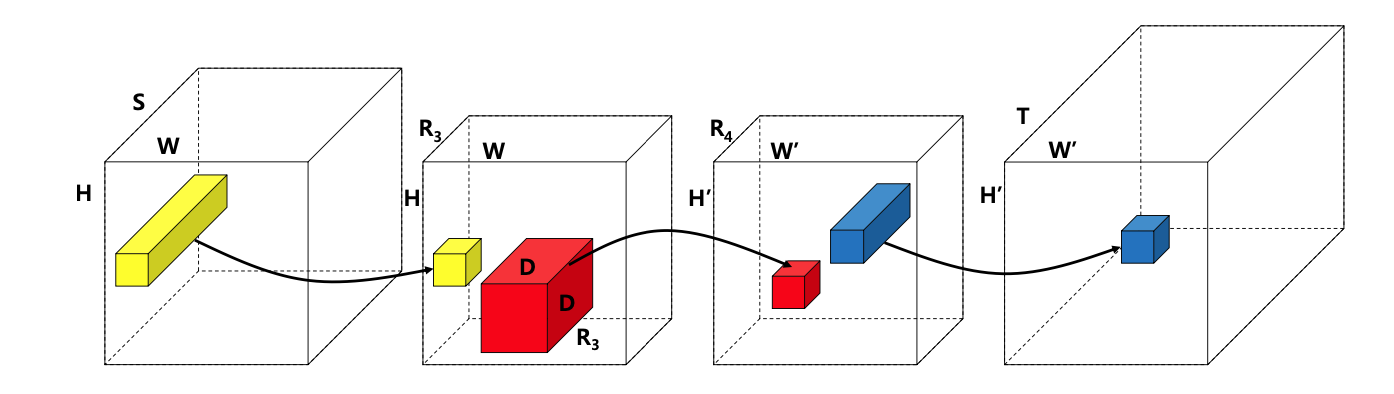
\includegraphics[width=\linewidth]{Pics/03_Previous_work/tuckerDecomp.png}
    \captionsetup{width=.95\linewidth}
    \caption{Taken from \cite{Kim2016}. The boxes correspond to the 3-dimensional tensors in the network with the frontal sides being the spatial dimensions. Each of the arrows show a linear mappings. The two middle tensors are the intermediate tensors with $R_3$ and $R_4$ being the ranks of the decomposition.}
    \label{fig:tuckerDecompConv}
\end{figure}

\subsection{Overall comparison of methods}
It seems that the biggest compression happens in the dense layers, since these are very heavy in number of parameters, on the other hand the convolution takes longer since there are more evaluations per parameter. In trying to speed up the CNN, the method using BTD proposed in \cite{Wang2016} seems to get the best results. On the VGG-16 network architecture\cite{Simonyan2015} they achieve an acceleration of $6.6 \times$, while the methods of Jaderberg et al. \cite{Jaderberg2014} and Kim et al. \cite{Kim2016} achieve $3.8 \times$ and $3.3\times$ respectively. The authors of the BTD method also discuss and test decomposing the first dense layer since this can be treated as a convolution with large filters. The method using CP-decomposition \cite{Lebedev2015} worked well, but did not seem to be scaleable.

% Outline:
% Speeding up the dense layer
% Speeding up the convolutional layer
% Speeding up the entire network
%\clearpage

%\section{Data} \label{tex:data}

In this thesis two different data sets will be used; the well-studied MNIST data set \cite{MNIST} of handwritten digits, and the relatively new THETIS data set \cite{Gourgari2013} of videos of tennis shots. The idea is to first apply the methods discussed later to the simpler MNIST data set, to make sure that it is working properly, followed by an application to the more complicated THETIS data set. This also makes it possible to examine the potentially different effect the methods discussed later will have on the speed-up. Each of the data set will be described in the following. 

\subsection{MNIST - Handwritten Digits}
The MNIST (Modified National Institute of Standards and Technology) data set \cite{MNIST} consists of 70,000 pictures\footnote{The 70,000 is split into 60,000 training pictures and 10,000 testing pictures} of handwritten digits from 0 through 9. Each picture is $28\times 28$ pixels and black/white which means that there is only one input channel. Each of the $28\cdot 28 = 784$ pixel values are intensities ranging from 0 (black) to 255 (white). The data set is formed by remixing samples from the earlier NIST data set, which consisted of both digits and characters. The MNIST samples would be picked out, standardized and normalized so they would all be the same size and have the same gray-values \cite{mnistdatabase}. The first 175 samples from the traning set of the MNIST database is shown in \autoref{fig:MNISTdata175}. 

\begin{figure}[H]
    \centering
    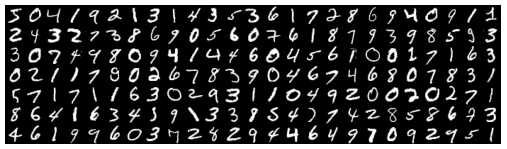
\includegraphics[width=\linewidth]{Pics/04_Data/MNIST.png}
    \caption{The first 175 samples of the MNIST data set of handwritten digits}
    \label{fig:MNISTdata175}
\end{figure}

\subsection{THETIS - Tennis Shot Videos}
The THETIS (Three dimEnsional TennIs Shots) data set consists of videos of 1980 tennis shots performed by both beginners and more experienced individuals \cite{Gourgari2013}. Each of the 12 types of shots types have been performed multiple times by each of the 55 individuals (31 beginners and 24 experts). Each shot consists of an RGB video, a depth video, a silhouette video, and both 2D and 3D skeleton videos. The videos have a resolution of $480\times 640$, while they vary in length (approximately 3-7 s). Since the skeleton extraction is not always successful, only 1217 of the shots have this feature. This means that the total number of videos in the data set is 8,374 resulting in a total playtime of 7 hours and 15 minutes. An overview of the 12 types of shots is given in \autoref{tab:typeOverviewTHETIS}, while an example of each of the five features is given in \autoref{fig:exampleVideosTennis}. 

\begin{table}
\centering
\caption{Overview of the 12 different types of tennis shots present in the THETIS data set.}
\label{tab:typeOverviewTHETIS}
\begin{tabular}{l|l|l|l}
\textbf{Forehand}    & \textbf{Backhand}     & \textbf{Service} & \textbf{Other} \\ \hline
Flat        & With 2 hands & Flat    & Smash \\
Slice       & Slice        & Slice   &       \\
Volley      & Volley       & Kick    &       \\
Open stands & Backhand     &         &      
\end{tabular}
\end{table}

\begin{figure}
    \centering
    \begin{subfigure}{.49\linewidth}
        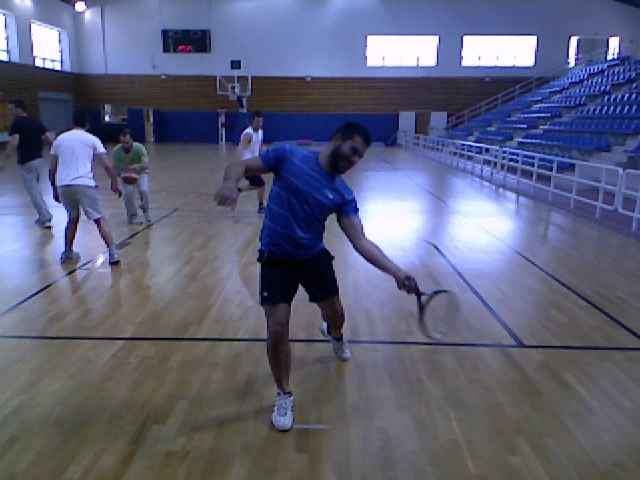
\includegraphics[width=\linewidth]{Pics/04_Data/frame53.jpg}
        \caption{Normal RGB video}
    \end{subfigure}
    \begin{subfigure}{.49\linewidth}
        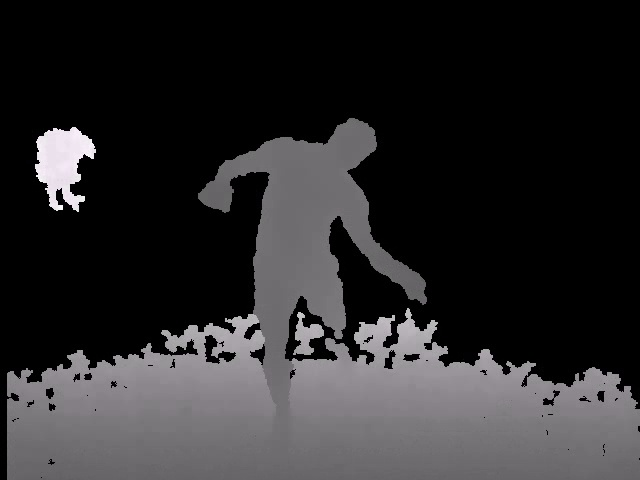
\includegraphics[width=\linewidth]{Pics/04_Data/frame53_depth.jpg}
        \caption{Depth video}
    \end{subfigure}
    \begin{subfigure}{.32\linewidth}
        
\includegraphics[width=\linewidth]{Pics/04_Data/frame53_mask.jpg}
        \caption{Silhouette}
    \end{subfigure}
    \begin{subfigure}{.32\linewidth}
        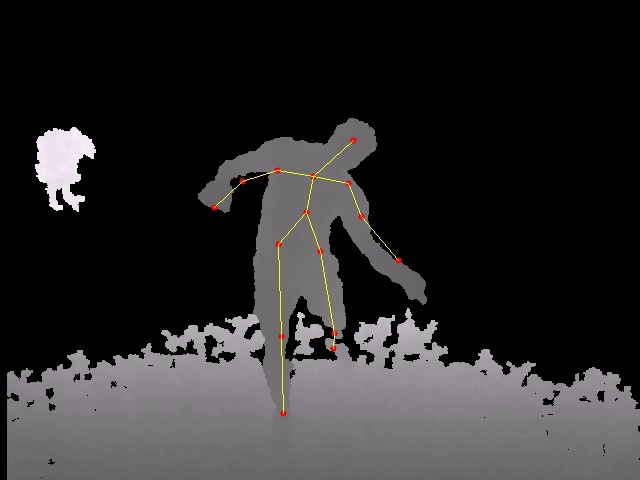
\includegraphics[width=\linewidth]{Pics/04_Data/frame53_skelet2D.jpg}
        \caption{2D Skeleton}
    \end{subfigure}
    \begin{subfigure}{.32\linewidth}
        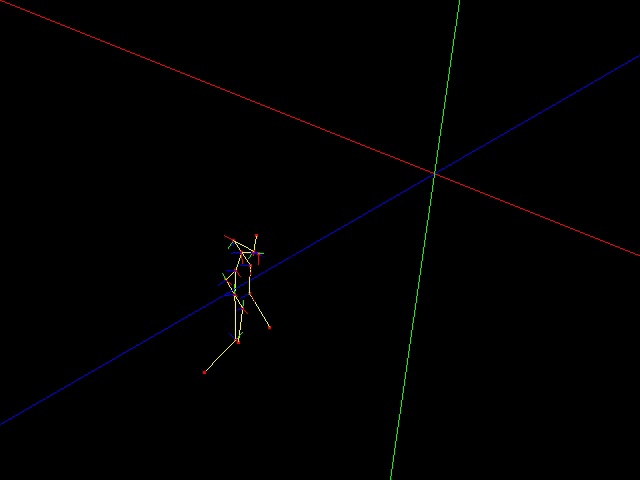
\includegraphics[width=\linewidth]{Pics/04_Data/frame53_skelet3D.jpg}
        \caption{3D skeleton}
    \end{subfigure}
    \caption{Example of the different videos that are given for each shot in the data set. Each of the pictures show the same frame in each of the videos of the same shot. Note that the 3D skeleton looks different since this is shown from a different angle. The 3D skeleton joint positions are also given numerically for each frame in the whole dataset.}
    \label{fig:exampleVideosTennis}
\end{figure}

Even though this data set is quite simple in relation to the real world, it is still complicated, especially in relation to the MNIST data set. The videos feature different individuals - both men and women, right handed and left handed, professionals and beginners. Even though the same type of shot is being performed by two individuals, they can look very different from each other. Also some of the videos are recorded in a sports arena with people doing different activities in the background as for instance yoga or basketball, while the others are recorded in a changing room with no noise at all.

\subsubsection{Pre-processing for THETIS}
In order to properly train on the THETIS data set, some preprocessing is needed. It is desirable to have the videos scaled down both in space and time, and to use more than just the RGB video from the data set. The depth video, which shows the depth information of the video on a gray-scale, only has one channel, and was easy to concatenate onto the RGB videos. This make the data set now have 4 input channels, which means more information to train on. The 4 channels of a single frame in the data set is illustrated in \autoref{fig:video_data_frame}. 
\begin{figure}
    \centering
    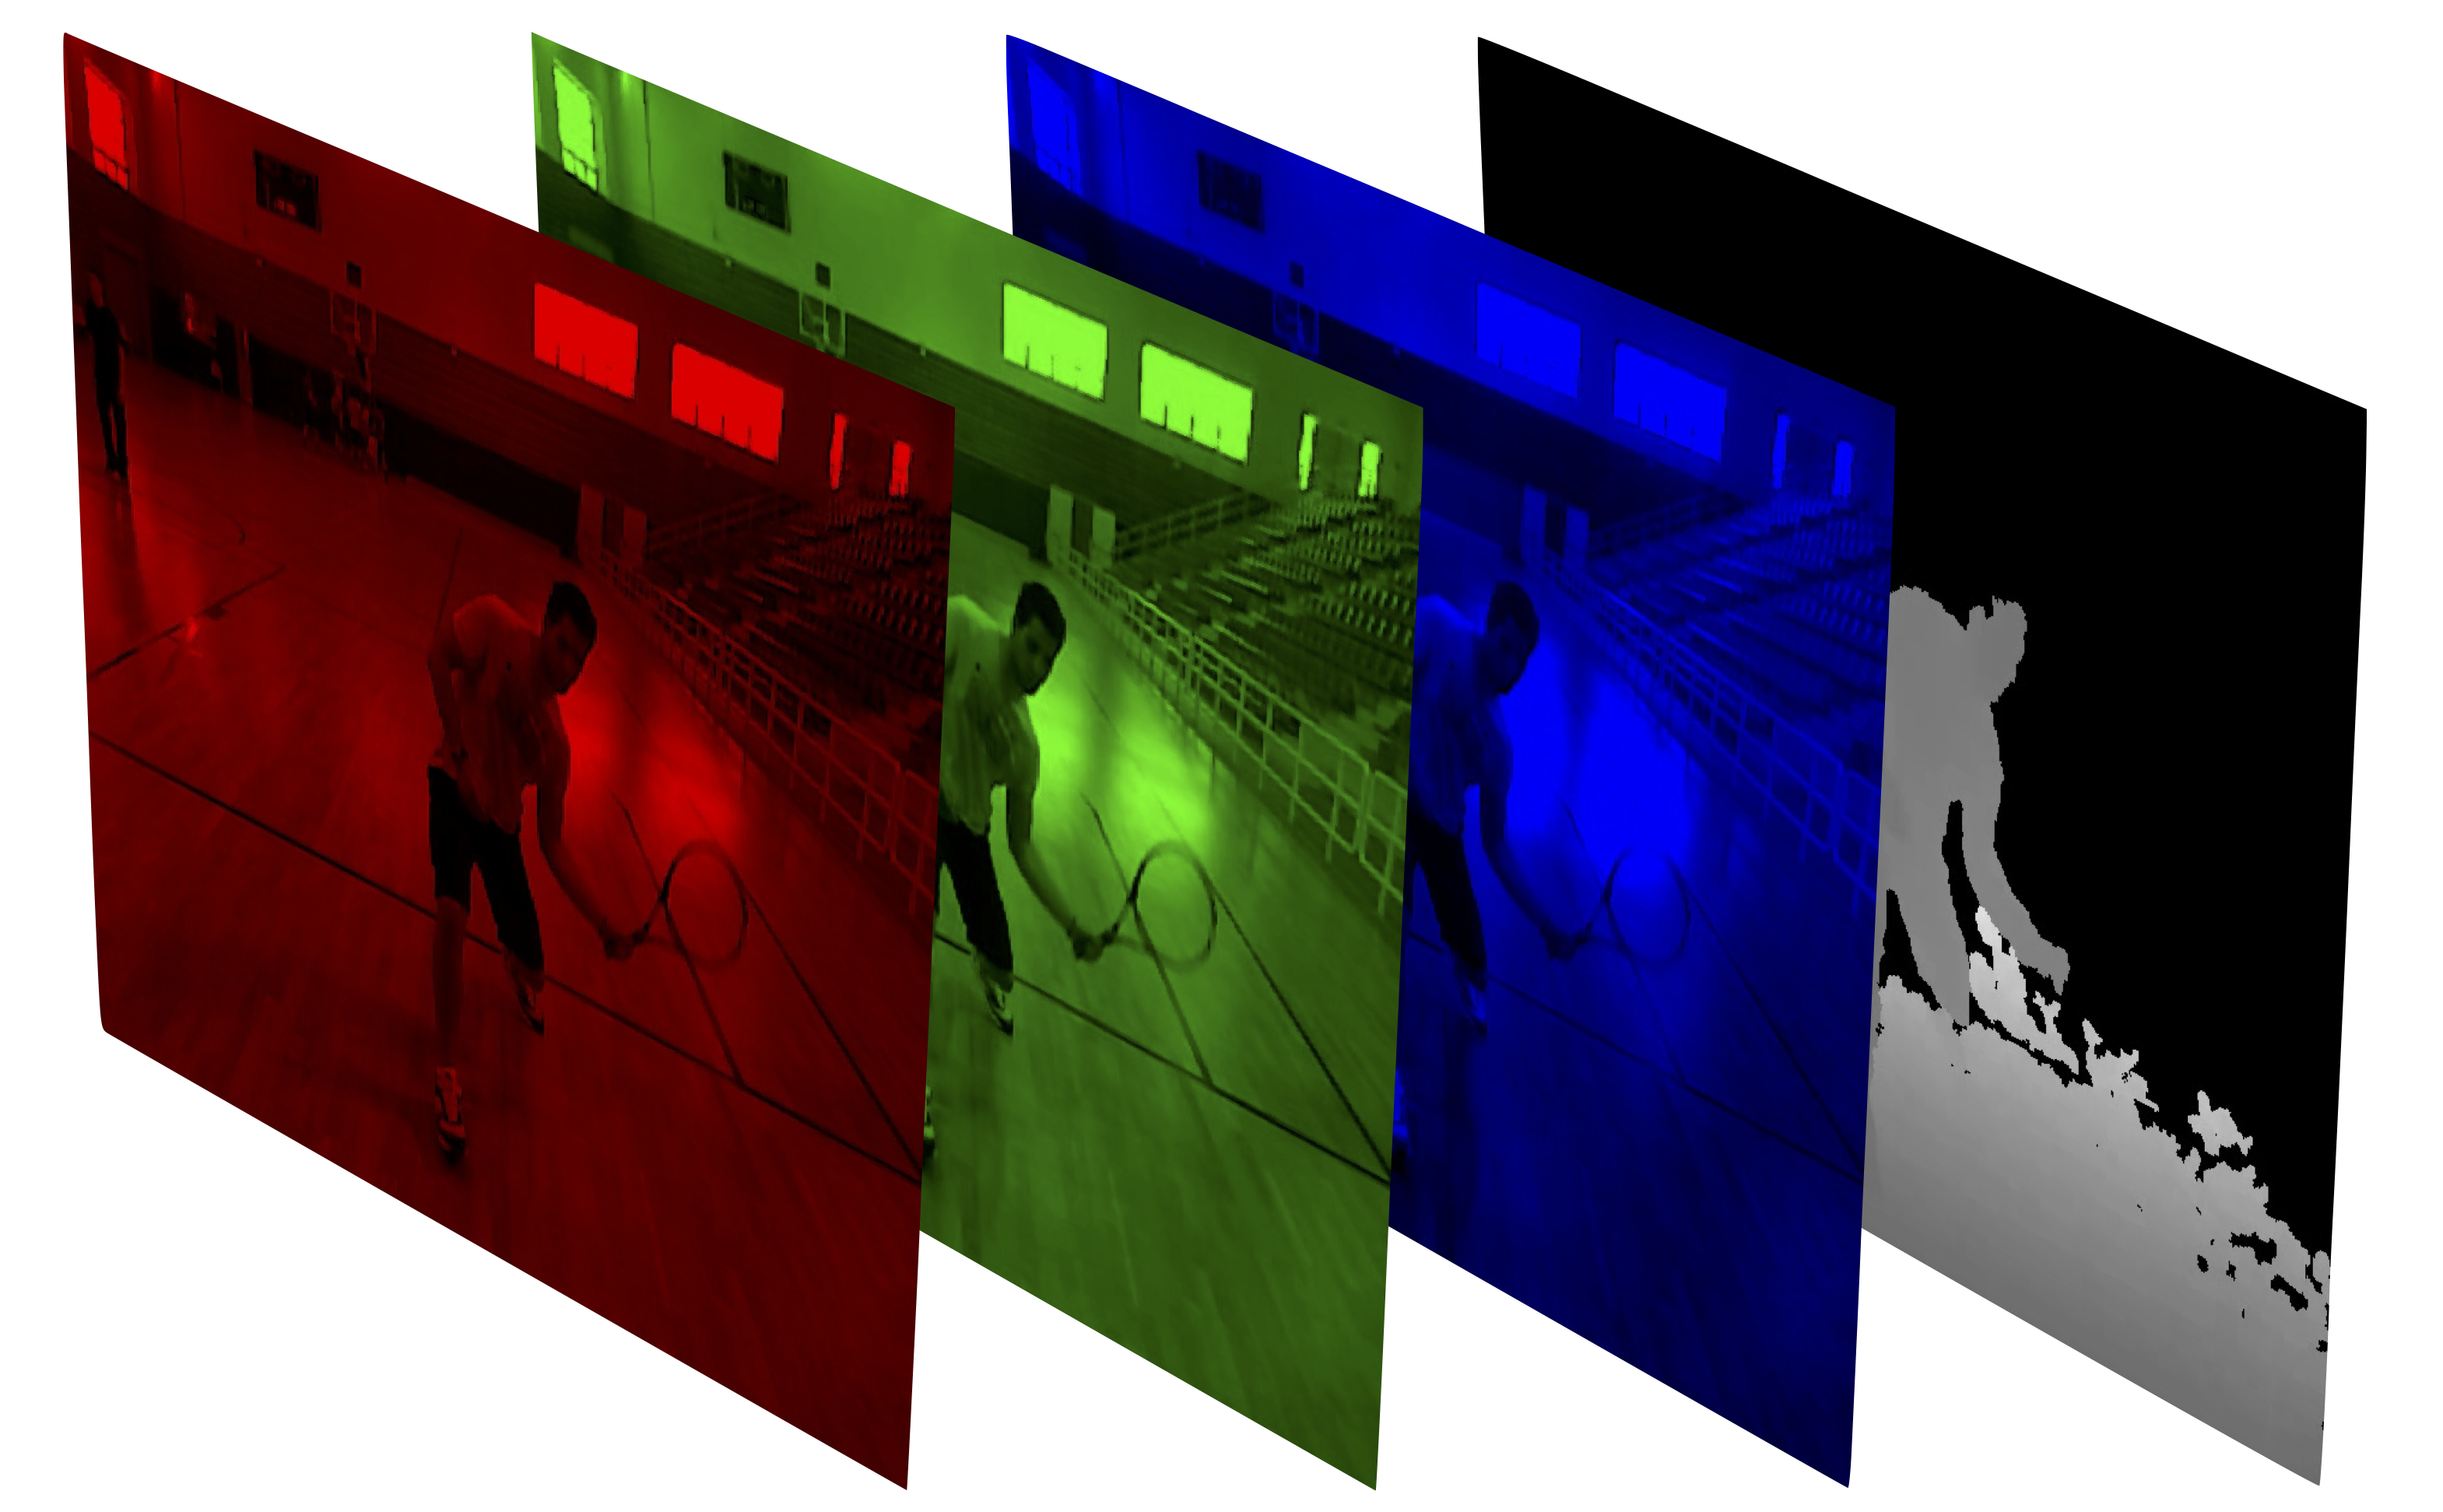
\includegraphics[width=.9\linewidth]{Pics/04_Data/RGBD.png}
    \caption{Each frame of the videos consists of 4 input channels; one red, one green, one blue, and one depth channel.}
    \label{fig:video_data_frame}
\end{figure}

One problems is that all the videos input into the network needs to have the same size, hence also the same length (number of frames). How this is typically ensured is by splitting the video into smaller pieces of the same length, and then running the algorithm on all the pieces and letting the majority of the smaller videos determine the class.\cite{Karpathy2014} While this is appropriate when trying to classify a general activity like running, swimming etc., it does not seem appropriate for this problem. This is due to the tennis shots being performed once per video, making the whole sequence a part of the shot. The problem was solved by manually inspecting the videos and assigning the time for the approximate midway through the shot. This assigned time is then used to extract the same number of frames on either side of the midway, making all videos have the same number of frames. This also has a standardizing effect, due to the middle of the shot being at the approximate same time in all videos. The number of frames is experimentally set to 14, making all videos 28 frames.

The last thing that was done to the data, was to decrease the resolution by a factor of 4 in each spatial dimension, i.e. from a resolution of $480\times 640$ to a resolution of $120\times 160$. This results in the number of pixels decreasing by a factor of 16 from 307,200 to 19,200, while still having a relatively high resolution that should be fine to train on. 

All of the above results in the THETIS observations having the size \begin{equation}
    (S \times F \times H \times W) = 4\times 28 \times 120 \times 160
\end{equation}
Where $S$ is the input channels, $F$ is the number of frames, $H$ is the height in pixels, and $W$ is the width in pixels.
%\clearpage

\section{Methodology} \label{tex:methodology}
Overall the methods examined in this thesis can be divided into two parts; namely those trying to decompose the input into a NN, and those decomposing the weights of a pre-trained NN with subsequent fine-tuning. In the following, the methods used within each of these parts will be discussed in detail. The Python library \textit{PyTorch}\cite{pytorch} will be used to implement and train all NN architectures, while all decomposition estimation will be executed using the Python library \textit{TensorLy}\cite{tensorly}. PyTorch provides a very popular application programming interface (API) for machine learning and tensor computing, which is easily accelerated using the graphics processing unit (GPU). TensorLy provides an API for tensor methods including the different decomposition methods described in \autoref{tex:decomp_methods}. TensorLy is also compatible with different back-ends\footnote{The back-end is the Python library that is responsible for low-level calculation and specification of the tensors. Typically \textit{NumPy}\cite{numpy} or \textit{PyTorch}\cite{pytorch}}, making it easy to combine with PyTorch. The algorithms used for estimating the decompositions in \textit{TensorLy} are given in \autoref{app:DecompEstimation}. 

After both the above mentioned methods have been discussed in detail, an overview of the architectures used in this thesis will be given, along with how to calculate the number of FLOPs used in different layers in a NN.

\subsection{Method 1 - Decomposing the Input}
In reality, tampering with data that is going to be learned is data preprocessing, hence decomposing the input is just a form of this. Data preprocessing is a vital part of almost all ML, because structured data of high quality is simply much easier to learn and to work with. Put in another way: "Garbage in, garbage out". In addition knowledge of the structure and the variance of the data often ease the algorithm development process. The decomposition algorithms seems appropriate for this task due to their ability to exploit the structure of the data.

The Tucker decomposition is believed to be suitable for data compression tasks \cite{Mørup2011}, which is why it seems natural to apply this method to the data before feeding it in to and training the NN. The purpose is to let the decomposition do some of the learning beforehand by exploiting the variance in the data. The Tucker-decomposition is flexible since it allows for decomposition of only a subset of the dimensions\footnote{This is also called a \textit{partial} Tucker decomposition}, and because it allows for specification of ranks for each dimension individually. Since the ranks correspond to the degree of flexibility, it is easy to choose how flexible the decomposition should be along each dimension. The rank would increase with the level of desired detail. This means that if the goal of the algorithm is to differentiate a small set of features, the rank would also be kept small along the relevant dimension.

Since the observations in each the given data sets can be stacked to form a 4 (MNIST) or 5 (THETIS) dimensional tensor, it is fairly straight forward to apply the Tucker decomposition. The algorithm discussed below will only cover the MNIST data set, since the expansion to videos is trivial (one more dimension). For $N$ MNIST observations, the stacked tensor $\tensor{X}$ of size $(N \times 1 \times 28 \times 28)$ will be reshaped to $(N\times 28 \times 28)$ due to the single input channel. The decomposition of the now 3rd order tensor becomes:
\begin{equation}
    \tensor{X}^{N\times 28 \times 28} \ \approx \  \tensor{G}^{L\times J \times K} \times_1 \bs{A}^{N\times L} \times_2 \bs{B}^{28 \times J} \times_3 \bs{C}^{28 \times K}
\end{equation}
Where $L, J$ and $K$ corresponds to the ranks in each of the dimensions. Here $\tensor{G}$ is the core of the decomposition, $\bs{A}$ corresponds to the loading matrix along the between-sample dimension, while $\bs{B}$ and $\bs{C}$ correspond to the loading matrices in each of the spatial dimensions. Since the goal is to learn the differences between the different classes (digits) in the data set, only the between-sample dimension will be decomposed. The so-called Tucker-1 decomposition of the first dimension is given by:
\begin{align}
    \tensor{X}^{N\times 28 \times 28} \ &\approx \  \tensor{G}^{L\times 28 \times 28} \times_1 \bs{A}^{N\times L} \times_2 \bs{I}^{28 \times 28} \times_3 \bs{I}^{28 \times 28} \\
    &\approx \tensor{G}^{L\times 28 \times 28} \times_1 \bs{A}^{N\times L}
\end{align}
This is equivalent to SVD using the unfolded representation with respect to the first dimension:
\begin{equation}
    \bs{X}_{(1)} = \bs{A} \bs{G}_{(1)}
    \label{eq:tuckerMNISTinput}
\end{equation}
Now the loading matrix $\bs{A}$ holds information about what differentiates the different samples using only $L$ features. These features will be used as the input into a very simple ANN, potentially lowering the number of input nodes dramatically if $L$ is kept small. The algorithm is illustrated in \autoref{fig:illustrationinputdecomp}.

In this project experiments will be made with different architectures for the simple ANN (i.e. number of hidden neurons in the hidden layer(s) $H$), along with different values of the rank $L$. The results will be provided and discussed in terms of the trade-off between computational speed and accuracy.

\begin{figure}
    \centering
    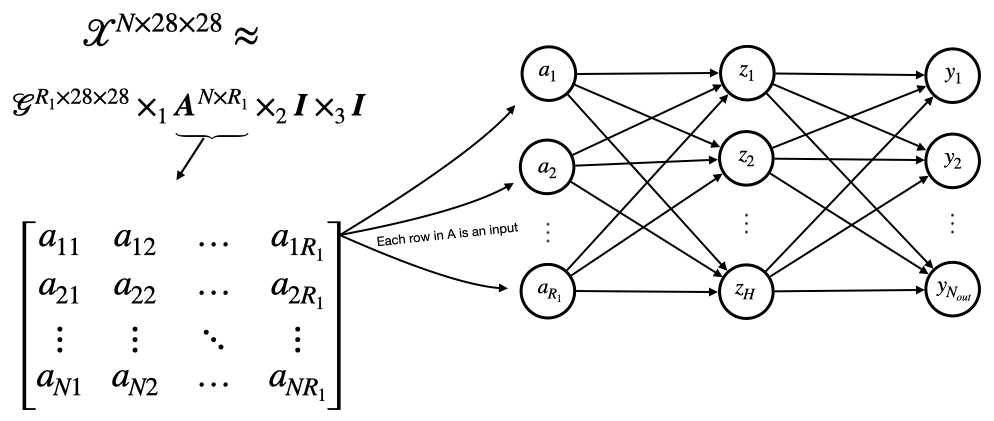
\includegraphics[width=\linewidth]{Pics/05_methodology/input_decomp_illustration.png}
    \captionsetup{width=.95\linewidth}
    \caption{Illustration of the algorithm that decomposes the input into the NN. The stacked data tensor will be decomposed along the between-sample dimension resulting in a loading matrix $\bs{A}$ which holds $L$ values for each observation, which will then be used as input into a simple ANN}
    \label{fig:illustrationinputdecomp}
\end{figure}

\subsubsection{Estimating the loadings for new data}
Since the testing data cannot be decomposed along with the training data, the loading matrix for the testing data will be estimated assuming the same core as for the training data. This way the decomposition is also a part of the training. Based on \eqref{eq:tuckerMNISTinput} the loading matrix for the test set can be estimated by multiplying with the pseudo-inverse of the matricized core:
\begin{equation}
    \bs{A}_{test} \approx {\bs{X}_{test}}_{(1)} \bs{G}_{(1)}^{\ \dagger}
\end{equation}
The two matrices $\bs{A}$ and $\bs{A}_{test}$ will be given as the input to the ANN as the training data and the validation/testing data respectively.


%%%%%%%%%%%%%%%%%%%%%%%%%%%%%%%%%%%%%%%%%%%%%%%%%%%%%%%%%%%%%%%%%%%%%%%%%%%%%%%%%%%%    
%%        Decomposing Pre-Trained Network    %%%%%%%%%%%%%%%%%%%%%%%%%%%%%%%%%%%%%%%
%%%%%%%%%%%%%%%%%%%%%%%%%%%%%%%%%%%%%%%%%%%%%%%%%%%%%%%%%%%%%%%%%%%%%%%%%%%%%%%%%%%%

\subsection{Method 2 - Compressing a Pre-Trained Network}
Using this approach is relatively easy to justify which is properly the reason why all the methods discussed in \autoref{tex:previous_work} use this approach. Pre-training a network makes it easier to ensure a network that works well, also because the training is often performed on powerful computers which allows for more complex networks. After the training is concluded the network is only decomposed to optimise the evaluation time in order to make it useful on platforms with less computation power. As discussed in \autoref{tex:previous_work} there are multiple approaches for this, but especially the methods using Tucker-decomposition and BTD seamed to be performing well and relatively straight-forward to implement and fine-tune.
The method used in this project builds on the work done by Kim et al. in \cite{Kim2016}, which is briefly discussed in \autoref{tex:sub_entire_network}.  Similar to the work done by Kim et al., Tucker-1 or Tucker-2 will be used for specific layers through the network. Kim et al. proposed method for compressing image convolutions, why the methods will be generalized to videos in the following. The advantage of using Tucker-decompositions is that they can be applied to each of the layers in the network, compressing everything at once before fine-tuning the whole network. In the following the methods of decomposing and changing the architecture of the layers of the network will be discussed. Due to the dissimilarities of the linear vs. the convolutional layer, each of these decompositions will be implemented individually for each type of layer. In the end, the full algorithm for compressing a whole network will be given.

\subsubsection{The linear / dense layer}
As explained in \autoref{tex:theory_NN} the dense layer with $N_{in}$ input neurons and $N_{out}$ output neurons in simply a matrix-vector product:
\begin{equation}
    \bs{y}^{N_{out}} = \bs{W}^{N_{out}\times N_{in}}\bs{x}^{N_in} + \bs{b}^{N_{out}}
    \label{eq:linearLayerTransformWOdecomp}
\end{equation}
Where $\bs{x}$ is the input, $\bs{y}$ is the input, $\bs{b}$ is the bias vector, and $\bs{W}$ is the weight matrix. The weight matrix is potentially big resulting in many parameters and high calculation time. The idea of the decomposed linear layer is to decompose the weight tensor into a set of smaller matrices that can be multiplied sequentially resulting in higher efficiency. The Tucker-1 and Tucker-2 decompositions of the weight matrix are given as:
\begin{align}
\texttt{Tucker-1}&: \quad \bs{W} \approx \bs{G} \times_1 \bs{A} \times_2 \bs{I} = \bs{A}\bs{G} \qquad \text{OR} \qquad \bs{W} \approx \bs{G} \times_1 \bs{I} \times_2 \bs{B} = \bs{G}\bs{B}^\top \\
\texttt{Tucker-2}&: \quad \bs{W} \approx \bs{G} \times_1 \bs{A} \times_2 \bs{B} = \bs{A}\bs{G}\bs{B}^\top 
\end{align}
Here $\bs{I}$ is the identity matrix and the core tensor $\bs{G}$ is a matrix due to the weight matrix $\bs{W}$ only having 2 dimensions. The type of Tucker-1 decomposition is chosen based on which dimension is to be decomposed.\footnote{Dense layers often go from many inputs to a fewer outputs why the input dimension might be more desirable to compress.} Inserting the decomposition of $\bs{W}$ in the linear transform \eqref{eq:linearLayerTransformWOdecomp} yields:
\begin{align}
     \bs{y}^{N_{out}} &\approx \bs{A}^{N_{out}\times R_A} \bs{G}^{R_A\times N_{in}} \bs{x}^{N_{in}} + \bs{b}^{N_{out}} \\
    \texttt{Tucker-1}: \qquad \quad \ \ &\text{OR} \nonumber \\
    \bs{y}^{N_{out}} &\approx \bs{G}^{N_{out}\times R_B} \bs{B}^{\top \  R_B\times N_{in}}\bs{x}^{N_{in}} + \bs{b}^{N_{out}} \\
    &\quad \nonumber \\
    \texttt{Tucker-2}: \quad \bs{y}^{N_{out}} &\approx \bs{A}^{N_{out}\times R_A} \bs{G}^{R_A\times N_{in}} \bs{B}^{\top  R_B\times N_{in}}\bs{x}^{N_{in}} + \bs{b}^{N_{out}}
\end{align}
Now looking at the number of multiplications needed to do each of the products from right to left gives the values in \autoref{tab:numberOfMultiplicationsLinearLayer}. For instance using the Tucker-1 compression uses $N_{in}R + RN_{out}=R(N_{out}+N_{in})$ multiplications to do the matrix-product. The table also shows the restrictions on the ranks to have less multiplications than the uncompressed version, hence to be more efficient.
\begin{table}
    \centering
    \captionsetup{width=.9\linewidth}
    \caption{The number of multiplications needed to do the matrix-vector product in the linear layer \eqref{eq:linearLayerTransformWOdecomp} with the weight matrix decomposed using Tucker-1 and Tucker-2. The matrix product is assumed to be calculated from right to left.}
    \begin{tabular}{l|c|c}
        \textbf{Method} & \textbf{\# Multiplications} & \textbf{Faster when:} \\ \hline
        Uncrompressed & $N_{out} N_{in}$ & - \\
        Tucker-1 & $R(N_{in} + N_{out})$ & $R < \frac{N_{out}N_{in}}{N_{out} + N_{in}}$\\
        Tucker-2 & $N_{in}R_B + R_BR_A + R_AN_{out}$ & $(N_{in}+R_A)(N_{out}+R_B) < 2 N_{in}N_{out}$
    \end{tabular}
    \label{tab:numberOfMultiplicationsLinearLayer}
\end{table}

What also makes this decomposition smart is that the sequence of matrix multiplications can be achieved by a sequence of 2 or 3 linear layers, where the loadings from the decomposition can be directly used as weights. This makes it straight-forward to adapt the layer into a decomposed version and to fine-tune. The concept is illustrated in \autoref{fig:diffNNlinearLayer}. The biases from the original layer will be added only to the last layer in the sequence of the decomposed version and they will not be modified in any way.
\begin{figure}
    \centering
    \begin{subfigure}{0.35\linewidth}
        \centering
        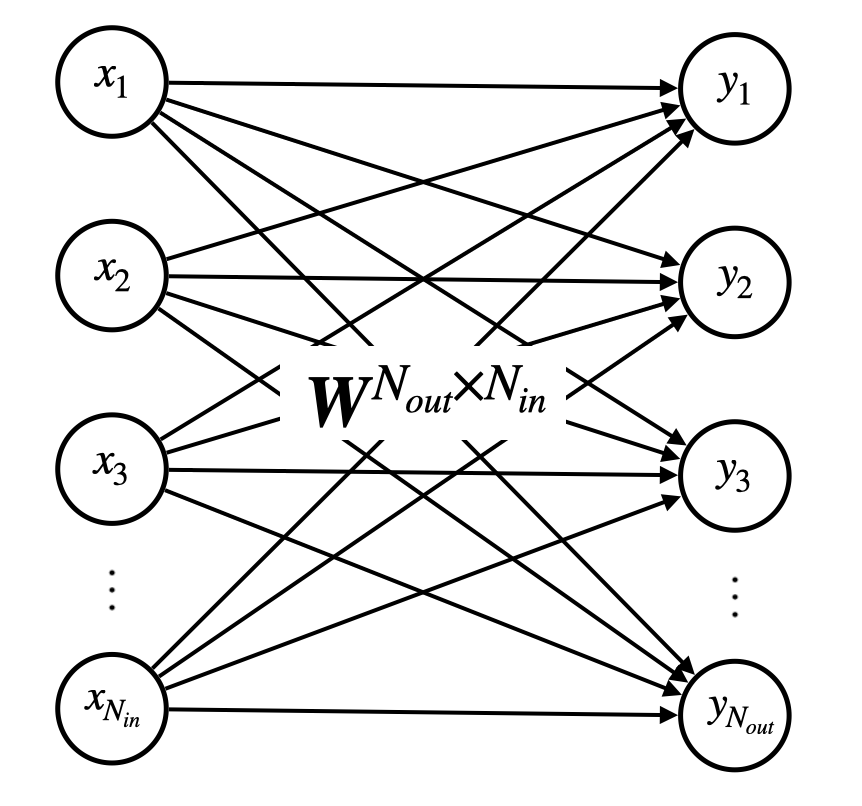
\includegraphics[width=\linewidth]{Pics/05_methodology/NNlinearLayer.png}
        \caption{Original linear layer}
    \end{subfigure}
    \begin{subfigure}{\linewidth}
        \centering
        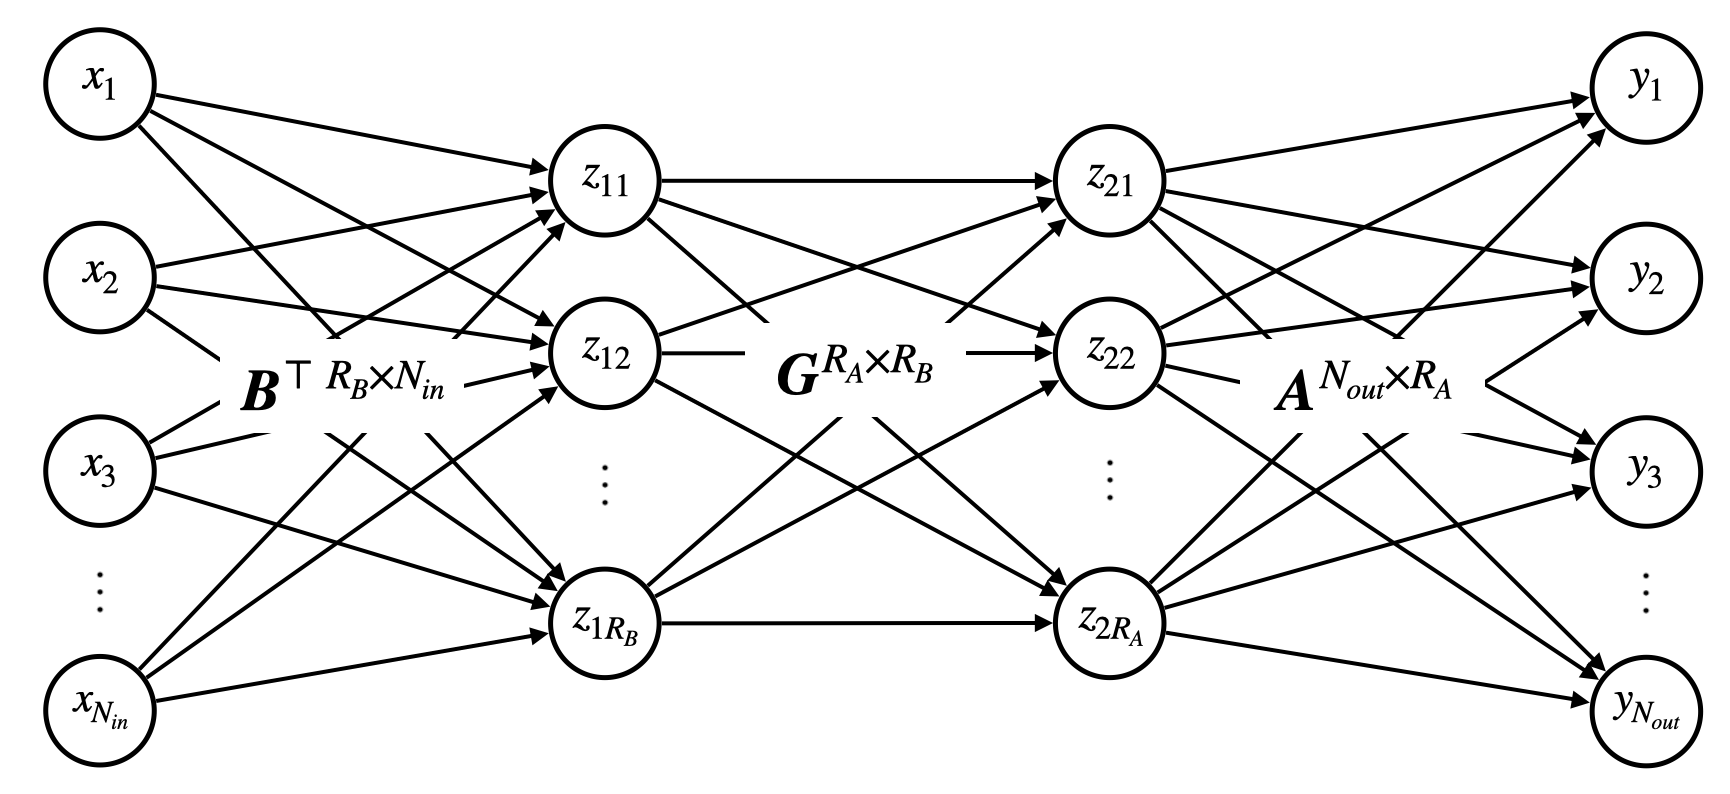
\includegraphics[width=.7\linewidth]{Pics/05_methodology/NNdecompLinearLayer.png}
        \caption{Sequence of linear layers resulting after decomposing $\bs{W}$}
    \end{subfigure}
    \captionsetup{width=.9\linewidth}
    \caption{Illustration of the difference between the original linear layer and the decomposed sequence of linear layers resulting after applying a Tucker-2 decomposition. The matrices $\bs{A}, \bs{B}$ and $\bs{G}$ are the resulting loading matrices and core respectively after decomposing the original weight matrix $\bs{W}$. The biases from the original layer will be added only to the last layer in the decomposed sequence.}
    \label{fig:diffNNlinearLayer}
\end{figure}

\subsubsection{The convolutional layer}
As explained in \autoref{tex:theory_NN} a convolution corresponds to calculating the result of applying a number of filters to every part of the input picture or video in space (and time). Applying the Tucker-decomposition to a convolutional layer implies turning it into a sequence of 3 (Tucker-2) or 2 (Tucker-1) smaller, less computational convolutions. The following method will only be discussed for videos, since the calculations are almost identical for lower dimensions. Kim et al. proposed a method for compressing an image filter in \cite{Kim2016}. In the following their method will be generalized to videos based on their derivations.

\paragraph{Tucker-2 decomposition of the convolutional kernel}
The convolution of an input tensor $\tensor{X}$ of size\footnote{Here and in the following $F$, $H$, $W$ are the number of frames, the height and the width of the video respectively. $S$ is the number of input channels.} $F\times H \times W \times S$ into an output tensor $\tensor{Y}$ of size $F'\times H' \times W' \times T$ is given by:
\begin{equation}
    \tensor{Y}(f', h', w', t) = \sum_{i=1}^{D_F} \sum_{j=1}^{D_H} \sum_{l=1}^{D_W} \sum_{s=1}^{S} \ \tensor{K}(i, j, l, s, t) \ \tensor{X}(f_i, h_j, w_l, s)
    \label{eq:3d_convolution}
\end{equation}
Where:
\begin{equation}
    f_i = \left(f' - 1\right) \Delta_F + i - P_F \qquad h_j =  \left(h' - 1\right) \Delta_H + j - P_H \qquad w_l =  \left(w' - 1\right) \Delta_W + l - P_W
\end{equation}
Where the $\Delta$s are the strides in each of the dimensions, the $P$s are the corresponding padding, and ($f'$, $h'$, $w'$, $t$) is the position in the output tensor $\tensor{Y}$. $\tensor{K}$ is the 5-dimensional convolutional kernel, i.e. the stack of 4-dimensional filters, and the $D$s are the filter sizes in each of the spatial and temporal dimensions. Now the Tucker-2 decomposition of $\tensor{K}$ in the input and output channel dimensions is expressed by:
\begin{equation}
\tensor{K}(i, j, l, s, t)=\sum_{r_{4}=1}^{R_{4}} \sum_{r_{5}=1}^{R_{5}} \tensor{C}(i, j, l, r_{4}, r_{5}) \ \boldsymbol{U}^{(4)}(s, r_{4}) \  \boldsymbol{U}^{(5)}(t, r_{5})
\end{equation}
Where $\tensor{C}$ is the core of the decomposition of size $D_F\times D_H \times D_W \times S \times T$ and the $\bs{U}$s are the loading matrices along the input and output dimensions respectively. Now substituting this expression into \eqref{eq:3d_convolution} gives:
\begin{equation}
    \tensor{Y}(f', h', w', t) = \sum_{i=1}^{D_F} \sum_{j=1}^{D_H} \sum_{l=1}^{D_W} \sum_{s=1}^{S} \sum_{r_{4}=1}^{R_{4}} \sum_{r_{5}=1}^{R_{5}} \tensor{C}(i, j, l, r_{4}, r_{5}) \ \boldsymbol{U}^{(4)}(s, r_{4}) \  \boldsymbol{U}^{(5)}(t, r_{5}) \ \tensor{X}(f_i, h_j, w_l, s)
\end{equation}
Rearranging, since not all factors depend on $s$, yields:
\begin{equation}
    \tensor{Y}(f', h', w', t) = \sum_{i=1}^{D_F} \sum_{j=1}^{D_H} \sum_{l=1}^{D_W} \sum_{r_{4}=1}^{R_{4}} \sum_{r_{5}=1}^{R_{5}} \tensor{C}(i, j, l, r_{4}, r_{5}) \ \boldsymbol{U}^{(5)}(t, r_{5}) \ \underbrace{\sum_{s=1}^{S} \boldsymbol{U}^{(4)}(s, r_{4}) \ \tensor{X}(f_i, h_j, w_l, s)}_{\large \tensor{Q}}
\end{equation}
Summing out $s$ yields an intermediate tensor $\tensor{Q}$ of size $F\times H \times W \times R_4$. Doing the same again:
\begin{equation}
    \tensor{Y}(f', h', w', t) = \sum_{i=1}^{D_F} \sum_{j=1}^{D_H} \sum_{l=1}^{D_W} \sum_{r_{4}=1}^{R_{4}} \sum_{r_{5}=1}^{R_{5}} \tensor{C}(i, j, l, r_{4}, r_{5}) \ \boldsymbol{U}^{(5)}(t, r_{5}) \  \tensor{Q} (f_i, h_j, w_l, r_4)
\end{equation}
Rearranging:
\begin{equation}
    \tensor{Y}(f', h', w', t) = \sum_{r_{5}=1}^{R_{5}} \ \boldsymbol{U}^{(5)}(t, r_{5}) \ \underbrace{\sum_{i=1}^{D_F} \sum_{j=1}^{D_H} \sum_{l=1}^{D_W} \sum_{r_{4}=1}^{R_{4}} \tensor{C}(i, j, l, r_{4}, r_{5})   \tensor{Q} (f_i, h_j, w_l, r_4)}_{\large \tensor{Q}'}
\end{equation}
Summing out everything but the output channels yields a new intermediate tensor $\tensor{Q}'$ of size $F' \times H' \times W' \times R_5$, and the convolution can now be expressed in terms of $\tensor{Q}'$:
\begin{equation}
    \tensor{Y}(f', h', w', t) = \sum_{r_{5}=1}^{R_{5}} \ \boldsymbol{U}^{(5)}(t, r_{5}) \ \tensor{Q}'(f', h', w', r_5)
\end{equation}
But now we have that the three intermediate tensors given by:
\begin{align}
    \tensor{Q}(f, h, w, r_4) &= \sum_{s=1}^{S} \boldsymbol{U}^{(4)}(s, r_{4}) \ \tensor{X}(f, h, w, s) \label{eq:Q}\\
    \tensor{Q'}(f', h', w', r_5) &= \sum_{i=1}^{D_F} \sum_{j=1}^{D_H} \sum_{l=1}^{D_W} \sum_{r_{4}=1}^{R_{4}} \tensor{C}(i, j, l, r_{4}, r_{5})   \tensor{Q} (f_i, h_j, w_l, r_4) \label{eq:Q'} \\
    \tensor{Y}(f', h', w', t) &=  \sum_{r_{5}=1}^{R_{5}} \ \boldsymbol{U}^{(5)}(t, r_{5}) \ \tensor{Q}'(f', h', w', r_5) \label{eq:Y}
\end{align}
correspond to the following sequence of simpler convolutions:
\begin{itemize}
    \item Eq. \eqref{eq:Q} - A $1\times 1$ convolution with $S$ input channels and $R_4$ output channels (the rank of the decomposition)
    \item Eq. \eqref{eq:Q'} - A $D_F \times D_H \times D_W$ convolution with $R_4$ input channels and $R_5$ output channels
    \item Eq. \eqref{eq:Y} - A $1\times 1$ convolution with $R_5$ input channels and $T$ output channels
\end{itemize}
So what this sequence is actually doing is first using the $1\times 1$ convolution to bring down the number of input channels to the 3D convolution, in order to perform the 3D convolution on a smaller set of input and output channels. In the end it uses the $1\times 1$ convolution to bring the now lower number of output channels back up to what it should be. This all results in a speed-up if the ranks are chosen to be small. Due to the challenge of illustrating a 4D tensor, the concept is illustrated in the 2D version (a picture) in \autoref{fig:tuckerDecompConv}. Like for the linear layer, the loadings of the decomposition of the kernel $\tensor{K}$ can be used directly as weights in the adapted architecture, and also the original biases will only be added to the last layer, while the other won't have biases.

\paragraph{Tucker-1 decomposition of the convolutional kernel}
In some situations it might not be beneficial to decompose both the input and the output channel dimensions, e.g. for an input image with only 3 input channels. The approach when doing the Tucker-1 decomposition is the same as for the Tucker-2 decomposition, however only one (relevant) rank is considered. This means that the resulting sequence have two smaller convolutions, and that there will be only two intermediate tensors corresponding to \eqref{eq:Q} and \eqref{eq:Q'} if the input channel dimension is to be decomposed, or \eqref{eq:Q'} and \eqref{eq:Y} for the output channel dimension. The derivations will be given for each of the dimensions in \autoref{tex:tucker1_conv_derivations}.

In order to choose the ranks so that the computation is faster, the number of multiplications needed for a forward push is now considered. We assume padding, i.e. same input and output sizes, since the difference between these is small - especially for small kernel sizes. The original convolution with $S$ input channels, $T$ output channels, a convolutional kernel with size $D_F\times D_H \times D_W$, and input/output size of $F\times H \times W$ uses:
\begin{equation}
    S \cdot T \cdot F \cdot H \cdot W \cdot D_F \cdot D_H \cdot D_W
\end{equation}
multiplications which quickly becomes a big number. We define:
\begin{equation}
    \Gamma = F \cdot H \cdot W \qquad \qquad \Lambda = D_F \cdot D_H \cdot D_W
    \label{eq:lambda_gamma_definition}
\end{equation}
To be used in the following such that the original convolution uses $S\cdot T \cdot \Gamma \cdot \Lambda$. The Tucker-1 decomposition of the convolution with rank $R$ uses:
\begin{equation}
S \cdot R \cdot \Gamma \cdot 1^3 + R\cdot T \cdot \Gamma \cdot \Lambda = R\cdot \Gamma \left( S + T\cdot \Lambda \right)
\end{equation}
multiplications if the decomposition is carried out on the input channels, and
\begin{equation}
    S \cdot R \cdot \Gamma \cdot \Lambda + R \cdot T \cdot \Gamma \cdot 1^3 = R \cdot \Gamma \cdot \left( S \cdot \Lambda + T \right)
\end{equation}
multiplications on the output channels. For the convolution using the Tucker-2 decomposition with ranks $R_1$ and $R_2$, the forward push use:
\begin{equation}
    S\cdot R_1 \cdot \Gamma \cdot 1^3 + R_1 \cdot R_2 \cdot \Gamma \cdot \Lambda + R_2 \cdot T \cdot \Gamma \cdot 1^3 = \Gamma \left( S\cdot R_1 + R_1\cdot R_2 \cdot \Lambda + R_2\cdot T \right)
\end{equation}
multiplications. \autoref{tab:number_multiplications_conv} shows how the ranks should be chosen in order for the compressions to have less multiplications than the original convolution, hence be faster.
\begin{table}
    \centering
    \captionsetup{width=.95\linewidth}
    \caption{Number of multiplications used for a forward push for a 3D convolution using different algorithms and how the ranks should be chosen so the compressions are faster. $\Lambda$ and $\Gamma$ are defined in \eqref{eq:lambda_gamma_definition}.}
    \begin{tabular}{l|c|c}
        \textbf{Method} & \textbf{\# Multiplications} & \textbf{Faster when} \\ \hline
        Original & $S\cdot T \cdot \Gamma \cdot \Lambda$ & - \\
        Tucker-1 (in) & $R\cdot \Gamma \left( S + T\cdot \Lambda \right)$ & $R < \frac{S\cdot T\cdot \Lambda}{S + T\cdot \Lambda}$  \\
        Tucker-1 (out) & $ R \cdot \Gamma \left( S \cdot \Lambda + T \right)$ & $R < \frac{S\cdot T \cdot \Lambda}{S\cdot \Lambda + T}$\\
        Tucker-2 & $\Gamma \left( S\cdot R_1 + R_1\cdot R_2 \cdot \Lambda + R_2\cdot T \right)$ & $S\cdot R_1 + R_1\cdot R_2 \cdot \Lambda + R_2\cdot T < S\cdot T \cdot \Lambda$
    \end{tabular}
    \label{tab:number_multiplications_conv}
\end{table}

\subsubsection{Rank selection}\label{tex:rank_selection}
There will be no all-round method for rank selection in this report. Where it is possible VBMF will be used to do the decomposition automatically as explained in \autoref{tex:VBMF}. In the cases where VBMF fails the ranks will be set experimentally be the same as the rank in using the other dimension for which it works. This is mostly for the linear layers, where the automatic method fails when trying to find the rank in the input channel dimension. The implementation of the VBMF is taken from \cite{VBMF_impl}.

\subsubsection{One-shot compression a an entire CNN using Tucker}
Using the different algorithms for compressing a single layer in the CNN and appropriate ranks, the algorithm for compressing a whole CNN is given in \autoref{alg:one_shot_tucker}. The algorithm is basically training an appropriate network, decomposing all the layers given the methods above, and then fine-tuning the new decomposed network. This one-shot compression is applied when referring to method 2.

\begin{algorithm} \caption{One-Shot Tucker Compression of a CNN} \label{alg:one_shot_tucker}
\begin{algorithmic}[1]
    \State $\texttt{net} \leftarrow $ define an appropriate CNN
    \State train $\texttt{net}$ using the given training data
    \State $\texttt{net\_dcmp} \leftarrow $ make a copy of $\texttt{net}$
    \For{each \textbf{convolutional} layer; $\texttt{layer}$ in $\texttt{net\_dcmp}$}
        \State $\tensor{K}_{\texttt{layer}} \leftarrow $ take out weight tensor
        \State $R_4, R_5 \leftarrow$ choose appropriate rank(s)
        \State $\tensor{G}, \ \ \bs{U}^{(4)}, \bs{U}^{(5)} \leftarrow $ Decompose $\tensor{K}_{\texttt{layer}}$ using relevant algorithm \Comment{Or just one $\bs{U}$}
        \State $\texttt{layer\_dcmp\_1} \leftarrow $ define new $1\times 1$ convolution \Comment{If applicable}
        \State $\texttt{layer\_dcmp\_2} \leftarrow $ define new 3D convolution
        \State $\texttt{layer\_dcmp\_3} \leftarrow $ define new $1\times 1$ convolution \Comment{If applicable}
        \State $\tensor{K}_{\texttt{layer\_dcmp\_1}} \leftarrow \bs{U}^{(4)}$ \Comment{If applicable}
        \State $\tensor{K}_{\texttt{layer\_dcmp\_2}} \leftarrow \tensor{G}$
        \State $\tensor{K}_{\texttt{layer\_dcmp\_3}} \leftarrow \bs{U}^{(5)}$ \Comment{If applicable}
        \State $\bs{b}_{\texttt{layer\_dcmp\_3}} \leftarrow \bs{b}_{\texttt{layer}}$ add the bias to the last layer \Comment{Or in the line above}
        \State $\texttt{layer} \leftarrow \texttt{sequence}(\texttt{layer\_dcmp\_1}, \  \texttt{layer\_dcmp\_2}, \ \texttt{layer\_dcmp\_3})$
    \EndFor
    \For{each \textbf{linear} layer; $\texttt{layer}$ in $\texttt{net\_dcmp}$}
        \State $\bs{W}_{\texttt{layer}} \leftarrow $ take out weight matrix of size $N_{out} \times N_{in}$
        \State $R_A, R_B \leftarrow $ choose appropriate rank(s)
        \State $\bs{G}, \bs{A}, \bs{B} \leftarrow $ decompose $\bs{W}_{\texttt{layer}}$ using relevant algorithm \Comment{Or just $\bs{A}$ or $\bs{B}$}
        \State $\texttt{layer\_dcmp\_1} \leftarrow $ define new $R_B \times N_{in}$ linear layer \Comment{If applicable}
        \State $\texttt{layer\_dcmp\_2} \leftarrow $ define new $R_A \times R_B$ linear layer \Comment{Or $R_B\times N_{in}$ or $N_{out}\times R_A$}
        \State $\texttt{layer\_dcmp\_3} \leftarrow $ define new $N_{out} \times R_A$ linear layer \Comment{If applicable}
        \State $\bs{W}_{\texttt{layer\_dcmp\_1}} \leftarrow \bs{B}$ \Comment{If applicable}
        \State $\bs{W}_{\texttt{layer\_dcmp\_2}} \leftarrow \bs{G}$
        \State $\bs{W}_{\texttt{layer\_dcmp\_3}} \leftarrow \bs{A}$ \Comment{If applicable}
        \State $\bs{b}_{\texttt{layer\_dcmp\_3}} \leftarrow \bs{b}_{\texttt{layer}}$ add the bias to the last layer \Comment{Or in the line above}
        \State $\texttt{layer} \leftarrow \texttt{sequence}(\texttt{layer\_dcmp\_1}, \ \texttt{layer\_dcmp\_2}, \ \texttt{layer\_dcmp\_3})$
    \EndFor
    \State train $\texttt{net\_dcmp}$ using the given training data \Comment{fine-tuning}
\end{algorithmic}
\end{algorithm}

\subsection{Architectures Used in This Thesis} \label{tex:architectures}
In order to assess the performance of the different methods used in this thesis, baselines need to be established. To do this original or uncompressed architectures need to be chosen, based on what have previously proved to be appropriate in the different cases, and what intuitively makes sense. The architectures for the two different parts mentioned earlier in this section will be discussed in the following.

\subsubsection{Method 1}
For the first method that decomposes the input different values of the rank $R$ will be tried, hence it is only the simple ANN architecture that will need to be determined. For both data sets only one hidden layer will be provided in order to assess the amount of assistance the decomposition of the input provides to the ANN. For MNIST the number of hidden units will be experimentally set to 20, while for THETIS this number will be 100. This means that the whole ANN will consist of $R$ input neurons, a hidden layer with 20 (MNIST) or 100 (THETIS) hidden neurons, and an output layer with 10 (MNIST) or 2 (THETIS) neurons. \autoref{fig:illustrationinputdecomp} illustrates this architecture perfectly with $L$ being the different ranks and $H = 20$ (MNIST) or $H=100$ (THETIS).

\subsubsection{Method 2}
For the second method that decomposes a pre-trained network, a 2D and 3D CNN is applied to each of the data set respectively. For MNIST the so-called \textit{LeNet-5} will be applied because it previously have shown good results for MNIST\cite{MNIST} and because it consists of a rather simple sequence of convolutions, pooling, and dense layers. The 3D version of the same architecture will be applied to THETIS, which is simply an extension of the convolutions (and pooling) to 3 dimensions (video) instead of 2. This gives the network the ability to learn not only the spatial features of the videos, but also the movement which is important in this case. Since the video problem is not to classify a general activity such as running or swimming, the whole movement needs to be considered in order for the network to stand a chance. The sizes of the filters have all been chosen using trial-and-error, and have not been optimised in any way, which means they should be considered experimental. An illustration of the two networks with all size information is given in \autoref{fig:architecture_choices}.
\begin{figure}
    \centering
    \captionsetup{width=.95\linewidth}
    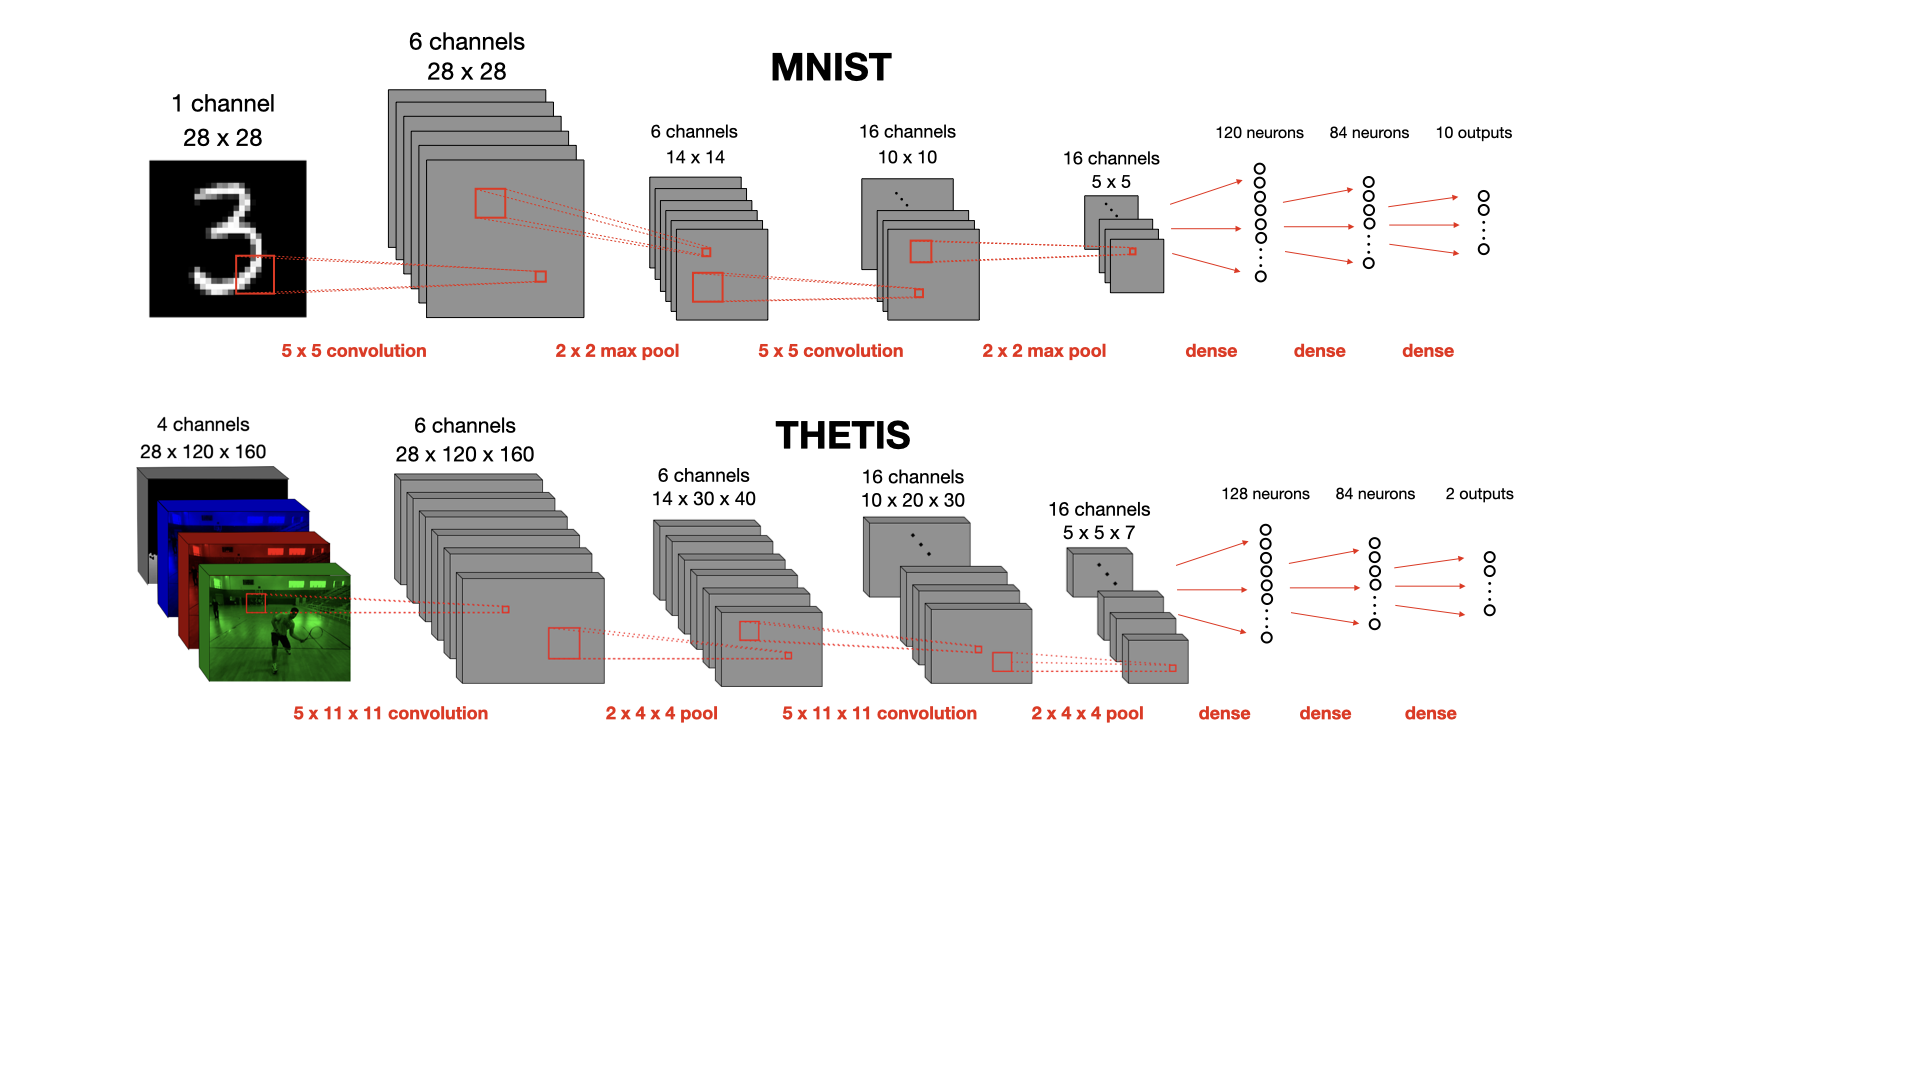
\includegraphics[width=\linewidth]{Pics/05_methodology/architecture_choice_illustration.png}
    \caption{The architectures used for each of the data sets in method 2. The size of the intermediate matrices or tensors are given above them along with the number of channels. The red operations are named underneath them along with the size of the operation}
    \label{fig:architecture_choices}
\end{figure}

The choice of which Tucker method to use for each layer is inspired by Kim et al.\cite{Kim2016} that would use Tucker-2 for all the convolutional layers (apart from the first) and the first dense layer, and Tucker-1 for the rest. An overview of which methods are used in the two architectures is given in \autoref{tab:Tucker_method_choice}. 
\begin{table}[H]
\centering
\caption{Which Tucker method (1 or 2) is applied the layers in each of the two architectures given in \autoref{fig:architecture_choices} for method 2. The last layer is not compressed in any of the two, due to the small size }
\label{tab:Tucker_method_choice}
\begin{tabular}{c|ccccc}
\begin{tabular}[c]{@{}c@{}}\textbf{Tucker-}\\ \textbf{method}\end{tabular} & Conv 1 & Conv 2 & Lin 1 & Lin 2 & Lin 3 \\ \hline
MNIST                                                    & 1      & 2      & 2     & 1     & -     \\
THETIS                                                   & 2      & 2      & 2     & 1     & -    
\end{tabular}
\end{table}

\subsection{Computational Complexity}\label{tex:computational_complexity}
In order to assess the theoretical performance of the different networks, we will make use of the number of floating point operations (FLOPs) that it takes for the network to do one forward push. We assume that the non-linearity (activation function) and the max-pooling computations for free, and only consider the FLOPs used in the dense and convolutional layers respectively.

\subsubsection{Dense layer}
For a dense layer with $N_{in}$ input neurons and $N_{out}$ output neurons, the forward push is calculated as a matrix-vector product. This means that it has $N_{in}N_{out}$ multiplications and $(N_{in}-1)N_{out}$ additions making it a total of:
\begin{equation}
    FLOPs_{lin} = N_{in}N_{out} + (N_{in}-1)N_{out} = N_{out} (2\cdot N_{in}-1)
\end{equation}
FLOPs to compute a forward push through the dense layer.

\subsubsection{Convolutional layer}
The number of FLOPs needed for a forward push in a convolutional layer is not as simple to compute due to the many hyper-parameters. The FLOPs will be based on the number of outputs, since this is direct result of the hyper-parameters. The following will only be computed for a 3D video convolutional kernel, since it generalises to an image kernel. Consider a convolutional layer with input channels $S$, output channels $T$, convolutional kernel $(D_F, D_H, D_W)$, and input size $(F, H, W)$. For every one of the $F' H' W' T$ output values, the filter is applied once which takes $D_F D_H D_W S$ multiplications and the same minus 1 additions. This makes the convolutional forward push use a total of:
\begin{equation}
    FLOPs_{conv} = T\cdot F'\cdot H'\cdot W'\cdot (2\cdot S \cdot D_F\cdot D_H\cdot D_W - 1)
\end{equation}
FLOPs to calculate. Here the output size of each dimension is calculated using the formula:
\begin{equation}
    out_{dim}(d, D, \Delta, P) = \frac{d - D + 2\cdot P}{\Delta} + 1
\end{equation}
Where $d$ is the input size, $D$ is the kernel size, $\Delta$ is the stride, and $P$ is the padding - all of the given dimension.

\subsubsection{Approximation of loadings matrix}
In method 1, the loading matrix $\bs{A}$ needs to be estimated for the testing observation $\tensor{X}^{I_1 \times I_2 \times \dots \times I_n}$, which is also a part of the time it takes to run the algorithm. The $\bs{A}$ is approximated by:
\begin{equation}
    \bs{A} \approx \bs{X}_{(1)} \bs{G}_{(1)}^{\dagger}
    \label{eq:estimation_of_loading_A}
\end{equation}
Where we assume that $\bs{G}_{(1)}^{\dagger}$ have already been estimated as a part of the training process and that the unfolding of $\tensor{X}$ is for free, which means that the approximation is a matrix-matrix product. $\bs{X}_{(1)}$ will have shape $I_1 \times \delta$ where $\delta = \prod_{k=2}^n I_k$, and $I_1$ is the number of input observations. $\bs{G}_{(1)}^{\dagger}$ will have shape $\delta \times R$ where $R$ is the rank of the decomposition. The total number of FLOPs it takes to approximate $\bs{A}$ for $I_1$ observations is given by:
\begin{equation}
    R \cdot I_1 (2\cdot \delta - 1), \qquad \quad \text{where} \quad \delta = \prod_{k=2}^n I_k
\end{equation}
Where $I_k$ is the size of the $k$th of the $n$ dimensions of $\tensor{X}$.
\clearpage

%\section{Results} \label{tex:results}
In this section results of applying the two methods discussed in the previous section will be given. Like discussing the methods in the previous section, the results will also be given in two parts. This is due to the two compression methods being so different in nature which means they cannot be directly compared. To compare the methods, a set of metrics will be applied to the original and compressed models respectively. The metrics include:
\begin{itemize}
    \item \textbf{Accuracy} - especially the accuracy drop is an important metric in comparing the compressed model to the full model, since there is trade-off between computational speed and accuracy
    \item \textbf{Number of Parameters} - how much space the model takes to store. This is important if small devices with limited storage space should be able to run the model
    \item \textbf{Theoretical speed} - based on the number of FLOPs, calculated using the formulas given in \autoref{tex:computational_complexity}. This is the actual number of calculations that is needed to perform a forward push. This should a good metric for the speed that can be calculated beforehand and used to predict the speed / speed-up of an algorithm.
    \item \textbf{Actual speed} - how long it takes to compute a forward push. Reported as the mean and standard deviation of many timings of the forward push. Due to potential differences in performance improvements, the methods will both be timed running on a CPU and GPU.
\end{itemize}
In the best case scenario, the actual speed improvement observed from timing the algorithms will be perfectly correlated with the calculated theoretical speed-up. Initially the results of method 1 will be given including observations from a small experiment, following this the results of applying method 2 will be given. Method 2 will also be applied to the well-known VGG-16 architecture\cite{Simonyan2015}, which have also been done by Kim et al.\cite{Kim2016}, however only on the convolutional layers.

\subsection{Method 1}
This is the method that decomposes the input into a NN. In order to get a better understanding of what happens when using this method, an experiment with only two classes for each data set and a rank of 2 will be carried out, and visual results will be given. Afterwards the results of using different ranks will be listed in order to assess performance differences.

\subsubsection{Experiment with low rank} \label{tex:result_experiment}
In the following an experiment is carried out to check whether the decomposition itself can carry much of the training. Since we have only 2 classes for the THETIS data set, and for the sake of the experiment 2 digits from the MNIST data set will be used. Since there are 2 classes in each data set, an initial rank of 2 will be experimentally chosen in the between sample dimension, since this also allows for a nice visualization of the loadings. The results for both the data set are described in the following.

\paragraph{Using MNIST 3s and 4s}
Only the MNIST observations depicting either a 3 or a 4 will be considered in this experiment. These digits are chosen due to their distinct shapes, hence ease of classification. Since the purpose is to make the algorithm find the differences between the two different digits, the spatial dimensions will not be decomposed. Using the experimental rank of 2, the decomposition of $N$ stacked 3s and 4s becomes:
\begin{equation}
    \tensor{X}^{N\times 28\times 28} \approx \tensor{G}^{2 \times 28 \times 28} \times_1 \bs{A}^{N\times 2} \qquad \Leftrightarrow \qquad \bs{X}_{(1)} \approx \bs{A}^{N\times 2} \ \bs{G}^{2 \times 28\cdot 28}_{(1)}
\end{equation}
Where $\bs{A}$ is the loading matrix in the dimension corresponding to different pictures. With the rank equal to 2, $\bs{A}$ holds 2 values per picture that should ideally be separating the two digits that is to be trained. \autoref{fig:decompExample3_4} shows how the decomposition of the first 100 training examples turns out. It seems the decomposition is able how to find the "general 3" and the "general 4", and then simply use the loadings of $\bs{A}$ to specify how much of each should be used to represent every observation. \autoref{fig:loadingAMatrix} shows a scatter-plot of the values of $\bs{A}$ colored to show the loadings corresponding to 3s and 4s respectively. There is some overlap between the two clusters, but it seems that they can be fairly distinguished. The mean of the loadings of the the 3s, 4s and overall respectively are also plotted in \autoref{fig:loadingAMatrix} and have been used to make the approximations shown in \autoref{fig:loadingsOfA}b-d. Here it is clear how an approximation is part 3, and part 4, and that the loadings specify how much.
\begin{figure}
    \centering
    \begin{subfigure}{0.45\linewidth}
        \centering
        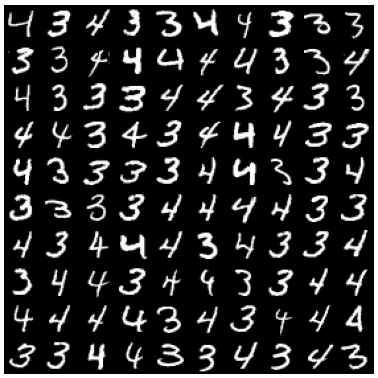
\includegraphics[width=\linewidth]{Pics/06_results/3_4_original.png}
        \captionsetup{width=.9\linewidth}
        \caption{Original MNIST training examples including only 3s and 4s.}
    \end{subfigure}
    \begin{subfigure}{0.45\linewidth}
        \centering
        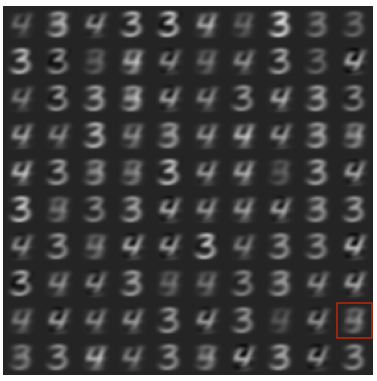
\includegraphics[width=\linewidth]{Pics/06_results/3_4_decomp.png}
        \captionsetup{width=.9\linewidth}
        \caption{Approximated versions of the training examples on the left, using the decomposition.}
    \end{subfigure}
    \captionsetup{width=.95\linewidth}
    \caption{MNIST training examples before and after decomposing with only rank 2 in the input dimension. Notice how the decomposed 3s and 4s look somehow standardized. It seems that every picture is a part standardized 3 and a part standardized 4. Notice how original digits that look relatively odd results in less certain approximation, e.g. the one highlighted with the red square.}
    \label{fig:decompExample3_4}
\end{figure}
\begin{figure}
    \centering
    \begin{subfigure}{0.99\linewidth}
        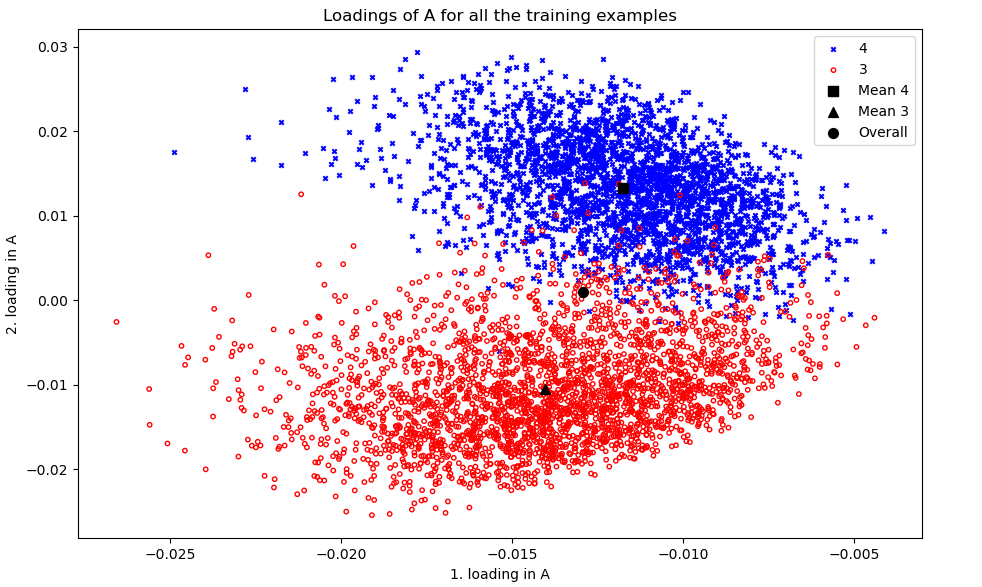
\includegraphics[width=\linewidth]{Pics/06_results/LoadingsOfAScatterMNIST.png}
        \caption{Scatter plot of the 2 loadings of the loading matrix $\bs{A}$ for the MNIST 3s and 4s respectively using rank 2 in the input dimension. The mean of the 2 clusters and overall is also marked with black.}
        \label{fig:loadingAMatrix}
    \end{subfigure}
    \begin{subfigure}{0.3\linewidth}
    \centering
        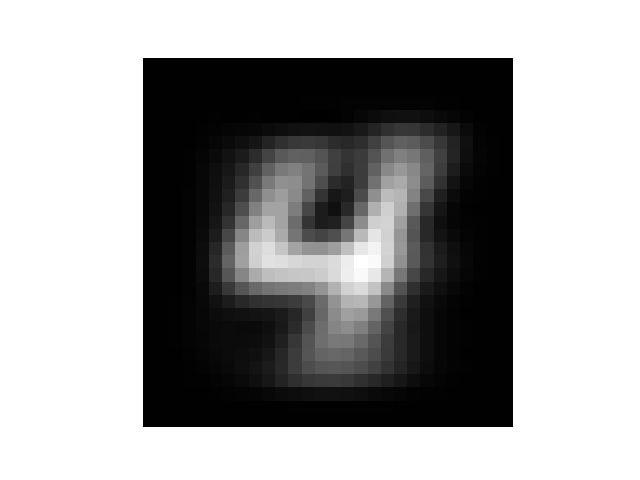
\includegraphics[width=.5\linewidth]{Pics/06_results/general4.png}
        \caption{The mean of 4s loadings}
    \end{subfigure}
    \begin{subfigure}{0.3\linewidth}
    \centering
        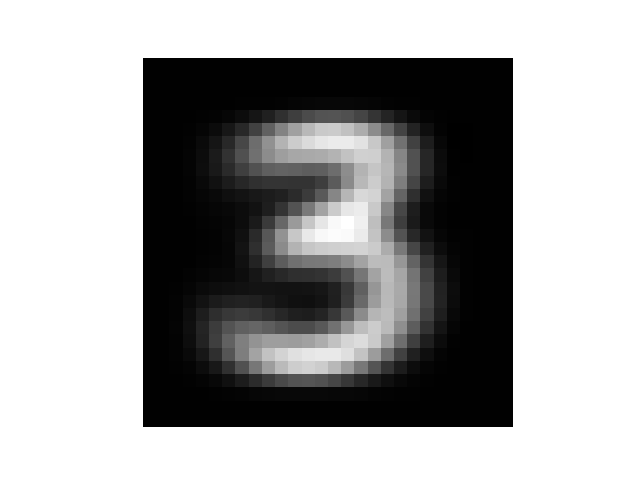
\includegraphics[width=.5\linewidth]{Pics/06_results/general3.png}
        \caption{The mean of 3s loadings}
    \end{subfigure}
    \begin{subfigure}{0.3\linewidth}
    \centering
        
\includegraphics[width=.5\linewidth]{Pics/06_results/general.png}
        \caption{The mean of all loadings}
        \label{Hej}
    \end{subfigure}
    \caption{Scatter plot of the 2 loadings of $\bs{A}$ for the MNIST 3s and 4s using rank 2 including mean in each of the clusters and overall. Using these means as loadings in the approximation gives the approximated "general" 3, 4 and overall given in \textbf{(b)-(d)}. Notice how the overall mean gives a mixture of a 3 and a 4.}
    \label{fig:loadingsOfA}
\end{figure}

In the end this all comes down to the loadings of $\bs{A}$ holding a great deal of information about which pictures are 3s and which are 4s. This information could be used as input into the NN instead of the actual pictures, potentially reducing the number of parameters dramatically (from 784 to 2 input neurons in this example). Training the network with this input and only 1 hidden neuron in the ANN achieved a testing accuracy of $\approx 97 \%$, which is good compared to simply using all the pixel values as inputs which achieved a testing accuracy of $\approx 95\%$.

\paragraph{Using THETIS forehand flat and backhand}
Following the same procedure as for the MNIST 3s and 4s the rank of the decomposition is experimentally set to 2. Stacking $N$ videos and decomposing with rank 2 in the between sample dimension, and leaving the remaining dimensions uncompressed, yield:
\begin{equation}
    \tensor{X}^{N\times 4 \times 28 \times 120 \times 160} \approx \tensor{G}^{2 \times 4 \times 28 \times 120 \times 160} \times_1 \bs{A}^{N\times 2}
\end{equation}
Now the loading matrix $\bs{A}$ holds 2 values for each observation that should ideally be separating the two types of shots. Making the scatter plot of the loadings from $\bs{A}$ colored according to the type of shot shows that this is however not the case. The scatter plot is shown in \autoref{fig:scatter_plot_THETIS}, where it is clear that there are two clusters. The clusters however do not separate the type of shot, but instead the location of the video. This means that the location gives the decomposition algorithm more information about the video than the type of shot. The mean of each of the clusters have been used to approximate the videos from which the frames given in \autoref{fig:scatter_plot_THETIS}(b) and (c) are taken from.
\begin{figure}
    \centering
    \begin{subfigure}{\linewidth}
        \centering
        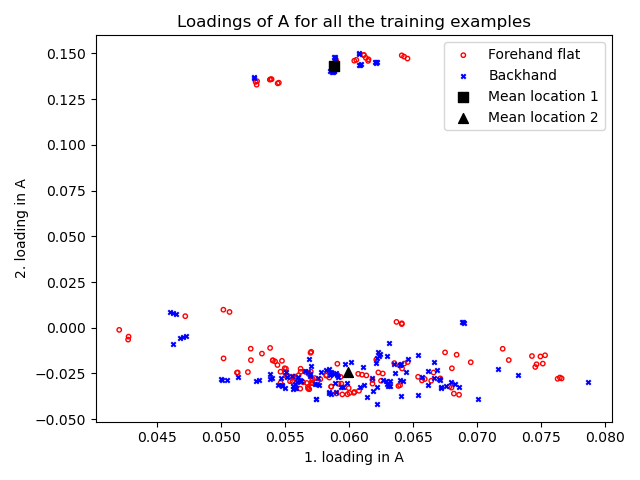
\includegraphics[width=0.64\linewidth]{Pics/06_results/scatter_loadings_THETIS.png}
        \captionsetup{width=.95\linewidth}
        \caption{Scatter plot of the loadings of $\bs{A}$ for the THETIS forehands and backhands. There seems to be two clusters, but they are not divided according to the shot type, but rather the background information. The mean of the two clusters that are given, have been used to approximate the videos in \textbf{(b)} and \textbf{(c)}.}
    \end{subfigure}
    \begin{subfigure}{.4\linewidth}
        \centering
        \captionsetup{width=.95\linewidth}
        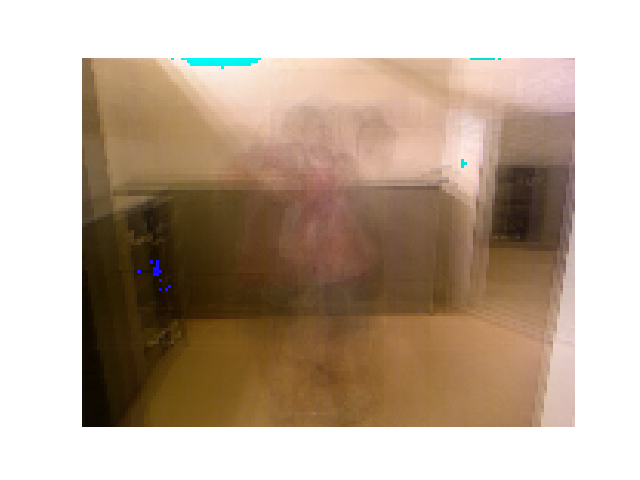
\includegraphics[width=\linewidth]{Pics/06_results/loc1.png}
        \caption{Approximation using the loadings of the mean of the little (top) cluster in \textbf{(a)}. This corresponds to one of the two locations (changing room).}
    \end{subfigure}
    \begin{subfigure}{.4\linewidth}
        \centering
        \captionsetup{width=.95\linewidth}
        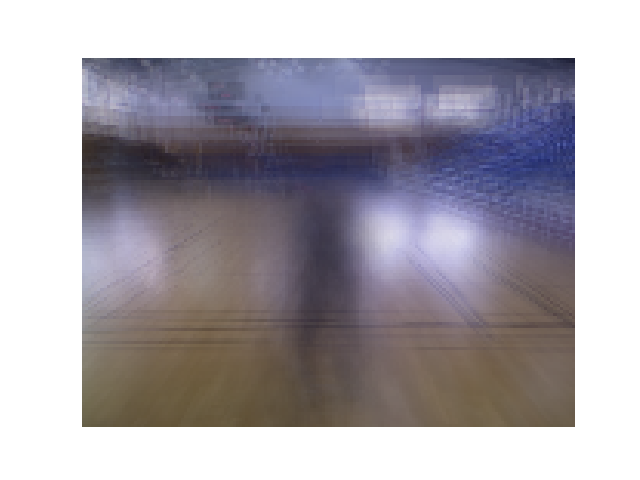
\includegraphics[width=\linewidth]{Pics/06_results/loc2.png}
        \caption{Approximation using the loadings of the mean of the big (bottom) cluster in \textbf{(a)}. This corresponds to one of the two locations (indoor arena).}
    \end{subfigure}
    \begin{subfigure}{.4\linewidth}
        \centering
        \captionsetup{width=.95\linewidth}
        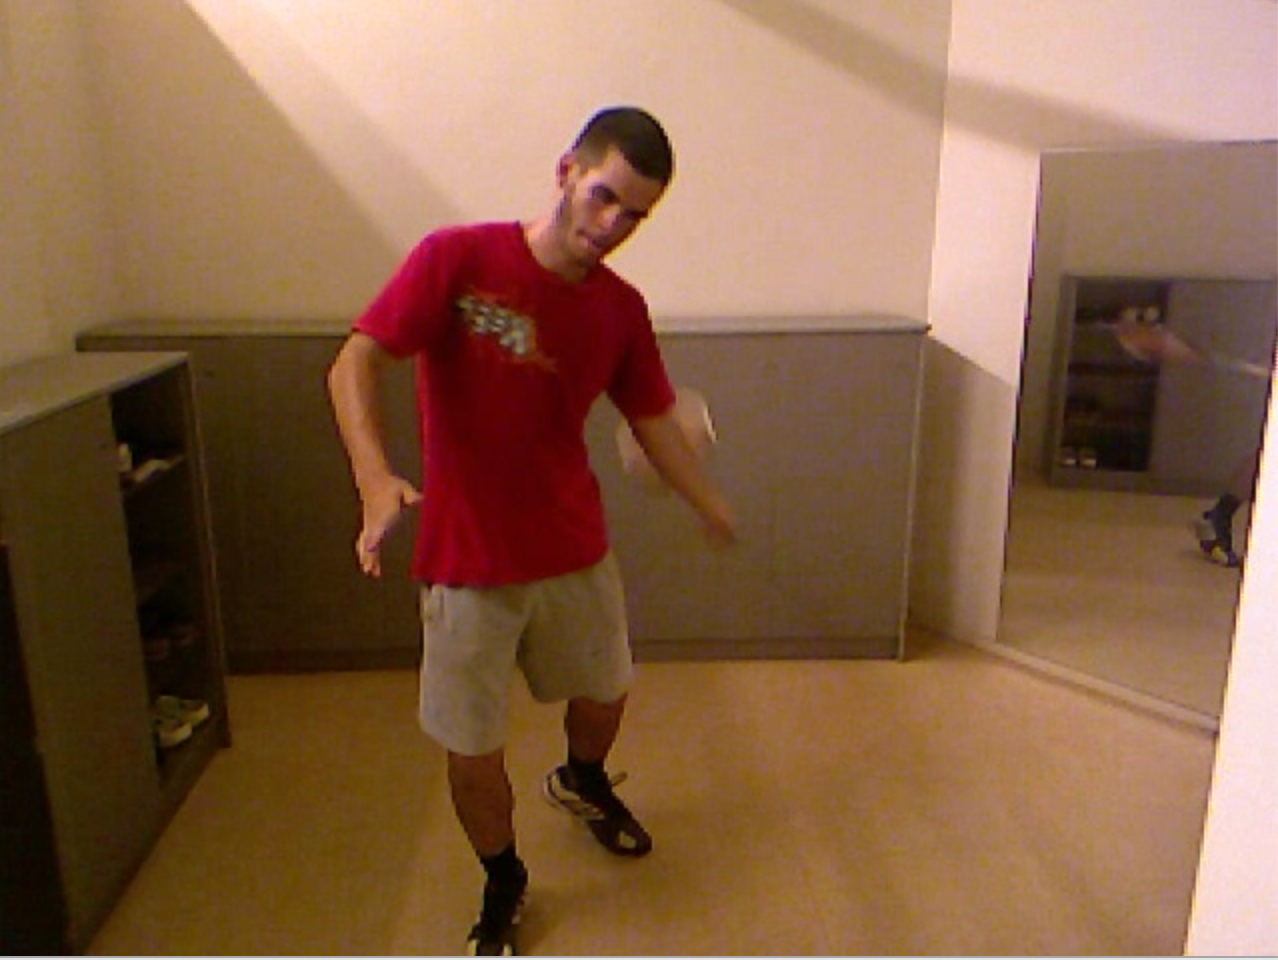
\includegraphics[width=.78\linewidth]{Pics/06_results/loc_1_real.png}
        \caption{An example of the changing room seen approximated in \textbf{(b)}}
    \end{subfigure}
    \begin{subfigure}{.4\linewidth}
        \centering
        \captionsetup{width=.95\linewidth}
        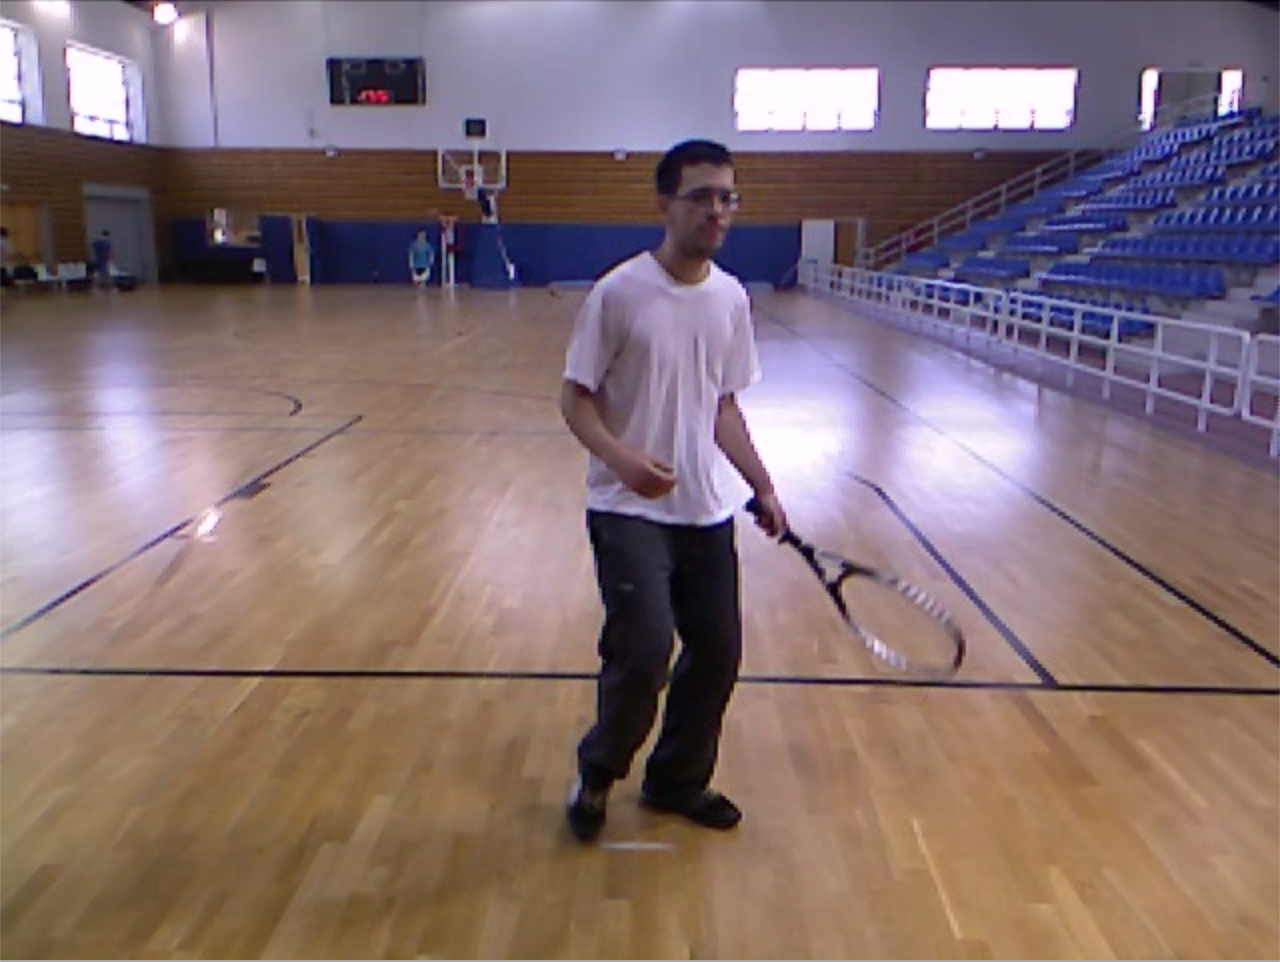
\includegraphics[width=.78\linewidth]{Pics/06_results/loc_2_real.png}
        \caption{An example of the indoor arena seen approximated in \textbf{(c)}}
    \end{subfigure}
    \caption{The loadings of $\bs{A}$ for the THETIS data illustrated by a scatter plot in \textbf{(a)}, and used to make the two approximation \textbf{(b)} and \textbf{(c)} by estimating the mean of each cluster seen in the scatter plot. It is clear how the two clusters in \textbf{(a)} separates the two locations, instead of the type of shot}
    \label{fig:scatter_plot_THETIS}
\end{figure}
This means that even though all the temporal information is given to the algorithm, the background is still the thing that separates the videos more. In order to differentiate the different type of shots more needs to be done as, e.g. increasing the rank allowing the algorithm to look for finer details or using some algorithm to remove the background. The accuracies after training this model are very low and not higher than a random classification.

\subsubsection{Results for MNIST}
The results for MNIST using the method that decomposes the input are given in \autoref{tab:res_input_MNIST}. Here the different models have been trained and timed, reporting the mean and the standard deviation of the time of 1,000 forward pushes through the network, assuming the core $\tensor{G}$ have already been matricized and inverted in \eqref{eq:estimation_of_loading_A}. Since the data is small and the models are all very fast, every forward push is conducted using 10 observations, which means that a total of 10,000 forward pushes have been timed. In \autoref{tab:res_input_MNIST}
the brackets holds the time of each of the two parts of the algorithm, i.e. estimating the input loadings ($\bs{A}$), and pushing these through the ANN. 

It seems that the compressed model exceeds the number of parameters and FLOPs of the full input model at the rank of around 20 where the accuracy is significantly lower than that of the original. Considering the timing on the CPU - the compressed model exceeds the full input model even earlier (at around 10-11). This all questions the applicability of the method - at least for very simple problems. The time using the GPU is rather constant, since the GPU is so fast, that a relatively small change in the number of calculations will not result in a big difference in the computation time. Actually the full input network is faster on the GPU than every one of the compressed models, meaning that the penalty of having multiple steps to the algorithm is too big.
\begin{table}
\footnotesize
\centering
\captionsetup{width=\linewidth}
\caption{The results of running the input decomposition method on the MNIST data set using different ranks for the decomposition. The time is reported as the mean and standard deviation of 1,000 samples where 10 observations are evaluated using the model. The numbers in brackets correspond to the break-down of the time of the estimation of the input loadings ($\bs{A}$) and the forward push through the network. The ratios are calculated between the attributes of the given compressed model and the model using the full input to the ANN. The accuracy seems to increase with along with the rank. Notice however that even though the rank of the decomposition is very high, the accuracy of the full input network is not reached - not even using 7.6 times the FLOPs (rank 150)}
\label{tab:res_input_MNIST}
\begin{tabular}{c|cccc|c}
\textbf{Rank}     & \textbf{\begin{tabular}[c]{@{}c@{}}Parameters\\ (K)\end{tabular}} & \textbf{\begin{tabular}[c]{@{}c@{}}FLOPs\\ (K)\end{tabular}} & \textbf{\begin{tabular}[c]{@{}c@{}}Time CPU\\ (ms)\end{tabular}}                  & \textbf{\begin{tabular}[c]{@{}c@{}}Time GPU\\ (ms)\end{tabular}}                  & \textbf{\begin{tabular}[c]{@{}c@{}}Accuracy\\ (\%)\end{tabular}} \\ \hline
\textbf{2}        & 1.83                                                              & 3.58                                                         & \begin{tabular}[c]{@{}c@{}}$1.481 \pm 0.025$ \\ $(= 0.904 + 0.647 )$\end{tabular} & \begin{tabular}[c]{@{}c@{}}$0.149 \pm 0.012$ \\ $(= 0.014 + 0.118 )$\end{tabular} & \textbf{33.61}                                                  \\
ratio             & 0.11                                                              & 0.11                                                         & 0.871                                                                             & 1.155                                                                             & 0.36                                                            \\ \hline
\textbf{5}        & 4.25                                                              & 8.41                                                         & \begin{tabular}[c]{@{}c@{}}$2.445 \pm 0.039$\\  $(= 1.885 + 0.551 )$\end{tabular} & \begin{tabular}[c]{@{}c@{}}$0.144 \pm 0.011$\\  $(= 0.013 + 0.115 )$\end{tabular} & \textbf{52.20}                                                  \\
ratio             & 0.25                                                              & 0.26                                                         & 1.438                                                                             & 1.116                                                                             & 0.55                                                            \\ \hline
\textbf{7}        & 5.86                                                              & 11.62                                                        & \begin{tabular}[c]{@{}c@{}}$3.114 \pm 0.047$ \\ $(= 2.525 + 0.565 )$\end{tabular} & \begin{tabular}[c]{@{}c@{}}$0.142 \pm 0.010$\\  $(= 0.013 + 0.113 )$\end{tabular} & \textbf{61.71}                                                  \\
ratio             & 0.35                                                              & 0.37                                                         & 1.832                                                                             & 1.101                                                                             & 0.65                                                            \\ \hline
\textbf{10}       & 8.27                                                              & 16.44                                                        & \begin{tabular}[c]{@{}c@{}}$1.660 \pm 0.033$\\  $(= 0.968 + 0.681 )$\end{tabular} & \begin{tabular}[c]{@{}c@{}}$0.141 \pm 0.011$\\  $(= 0.013 + 0.113 )$\end{tabular} & \textbf{67.55}                                                  \\
ratio             & 0.50                                                              & 0.52                                                         & 0.976                                                                             & 1.093                                                                             & 0.72                                                            \\ \hline
\textbf{15}       & 12.30                                                             & 24.48                                                        & \begin{tabular}[c]{@{}c@{}}$1.906 \pm 0.035$ \\ $(= 1.372 + 0.527 )$\end{tabular} & \begin{tabular}[c]{@{}c@{}}$0.141 \pm 0.011$\\  $(= 0.013 + 0.113 )$\end{tabular} & \textbf{72.14}                                                  \\
ratio             & 0.74                                                              & 0.77                                                         & 1.121                                                                             & 1.093                                                                             & 0.76                                                            \\ \hline
\textbf{20}       & 16.32                                                             & 32.51                                                        & \begin{tabular}[c]{@{}c@{}}$1.965 \pm 0.031$\\  $(= 1.354 + 0.598 )$\end{tabular} & \begin{tabular}[c]{@{}c@{}}$0.142 \pm 0.011$\\  $(= 0.014 + 0.113 )$\end{tabular} & \textbf{79.41}                                                  \\
ratio             & 0.98                                                              & 1.02                                                         & 1.156                                                                             & 1.101                                                                             & 0.84                  \\ \hline
\textbf{30}       & 24.37                                                             & 48.58                                                        & \begin{tabular}[c]{@{}c@{}}$2.397 \pm 0.035$ \\ $(= 1.785 + 0.599 )$\end{tabular} & \begin{tabular}[c]{@{}c@{}}$0.142 \pm 0.011$\\  $(= 0.015 + 0.115 )$\end{tabular} & \textbf{74.66}                                                  \\
ratio             & 1.46                                                              & 1.53                                                         & 1.410                                                                             & 1.101                                                                             & 0.79                                                            \\ \hline
\textbf{40}       & 32.42                                                             & 64.65                                                        & \begin{tabular}[c]{@{}c@{}}$2.298 \pm 0.039$ \\ $(= 1.756 + 0.528 )$\end{tabular} & \begin{tabular}[c]{@{}c@{}}$0.144 \pm 0.011$ \\ $(= 0.024 + 0.116 )$\end{tabular} & \textbf{74.89}                                                  \\
ratio             & 1.94                                                              & 2.04                                                         & 1.352                                                                             & 1.116                                                                             & 0.79                                                            \\ \hline
\textbf{50}       & 40.47                                                             & 80.72                                                        & \begin{tabular}[c]{@{}c@{}}$3.005 \pm 0.043$\\  $(= 2.242 + 0.752 )$\end{tabular} & \begin{tabular}[c]{@{}c@{}}$0.146 \pm 0.013$\\  $(= 0.025 + 0.114 )$\end{tabular} & \textbf{81.56}                                                  \\
ratio             & 2.43                                                              & 2.54                                                         & 1.768                                                                             & 1.132                                                                             & 0.86                                                            \\ \hline
\textbf{70}       & 56.57                                                             & 112.86                                                       & \begin{tabular}[c]{@{}c@{}}$3.661 \pm 0.047$\\  $(= 3.042 + 0.581 )$\end{tabular} & \begin{tabular}[c]{@{}c@{}}$0.144 \pm 0.010$ \\ $(= 0.022 + 0.115 )$\end{tabular} & \textbf{75.13}                                                  \\
ratio             & 3.39                                                              & 3.56                                                         & 2.154                                                                             & 1.116                                                                             & 0.80                                                            \\ \hline
\textbf{100}      & 80.72                                                             & 161.07                                                       & \begin{tabular}[c]{@{}c@{}}$4.796 \pm 0.067$ \\ $(= 3.897 + 0.823 )$\end{tabular} & \begin{tabular}[c]{@{}c@{}}$0.144 \pm 0.011$ \\ $(= 0.027 + 0.114 )$\end{tabular} & \textbf{83.98}                                                  \\
ratio             & 4.84                                                              & 5.08                                                         & 2.821                                                                             & 1.116                                                                             & 0.89                                                            \\ \hline
\textbf{150}      & 120.97                                                            & 241.42                                                       & \begin{tabular}[c]{@{}c@{}}$6.664 \pm 0.086$\\  $(= 5.655 + 0.849 )$\end{tabular} & \begin{tabular}[c]{@{}c@{}}$0.145 \pm 0.012$\\  $(= 0.034 + 0.115 )$\end{tabular} & \textbf{83.65}                                                  \\
ratio             & 7.25                                                              & 7.61                                                         & 3.920                                                                             & 1.124                                                                             & 0.89                                                            \\ \hline
\textbf{Full input} & 16.68                                                             & 31.73                                                        & $1.700 \pm 0.052 $                                                                & $0.129 \pm   0.013$                                                               & \textbf{94.44}                                                 
\end{tabular}
\end{table}

\subsubsection{Results for THETIS}
The results for THETIS are given in \autoref{tab:res_input_THETIS}. The time is given as the mean and standard deviation of the time based on 1,000 forward pushes through the different models, assuming the core $\tensor{G}$ have already been matricized and inverted in \eqref{eq:estimation_of_loading_A}. The brackets holds the time broken down into the two parts - estimating the loading matrix and pushing through the ANN.

Interestingly the accuracy of the decomposed model actually exceed that of the full input model when the rank is chosen big (150). Unfortunately the computational complexity and the computation time are both exceeded at this point. The compressed model exceed the computational complexity and time (CPU) at a rank around 100, where the accuracy does not match that of the full input model. This fact casts doubt on the functionality of this method. When running on the GPU the computation time is exceeded at an even lower rank, which could be due to the GPU being more penalized by the split into two steps as was also noted for the MNIST data set. 

Another thing to notice is that the estimation of the loading matrix accounts for the majority of the computation time by far. This is due to the estimation of the loadings being a rather big matrix-matrix product, since it gets the full input ($>2$ M values).
\begin{table}
\centering
\caption{Results for running the input decomposition algorithm on the THETIS data set using different ranks for the decomposition. The time is given as the mean and standard deviation of 1,000 forward pushes of 1 observation for each model. The numbers in brackets correspond to the break-down of the time of the estimation of the input loadings ($\bs{A}$) and the forward push through the network. The ratios are calculated between the attributes of the given compressed model and the model simply using the full input into the ANN. Notice how the accuracy of the original network is not reached before the rank is 150, exceeding the complexity and time by around 50 \% (73\% for GPU)}
\label{tab:res_input_THETIS}
\footnotesize
\begin{tabular}{c|cccc|c}
\textbf{Rank}     & \textbf{\begin{tabular}[c]{@{}c@{}}Parameters\\ (M)\end{tabular}} & \textbf{\begin{tabular}[c]{@{}c@{}}FLOPs \\ (M)\end{tabular}} & \textbf{\begin{tabular}[c]{@{}c@{}}Time CPU \\ (ms)\end{tabular}}                     & \textbf{\begin{tabular}[c]{@{}c@{}}Time GPU \\ (ms)\end{tabular}}                 & \textbf{\begin{tabular}[c]{@{}c@{}}Accuracy \\ (\%)\end{tabular}} \\ \hline
\textbf{30}       & 64.52                                                             & 129.03                                                        & \begin{tabular}[c]{@{}c@{}}$30.534 \pm 0.325$ \\ $(= 30.322 + 0.081 )$\end{tabular}   & \begin{tabular}[c]{@{}c@{}}$0.340 \pm 0.073$ \\ $(= 0.246 + 0.209 )$\end{tabular} & \textbf{70}                                                      \\
ratio             & 0.30                                                              & 0.30                                                          & 0.33                                                                                  & 0.33                                                                              & 0.76                                                             \\ \hline
\textbf{40}       & 86.02                                                             & 172.04                                                        & \begin{tabular}[c]{@{}c@{}}$38.481 \pm 0.371$\\  $(= 38.085 + 0.087 )$\end{tabular}   & \begin{tabular}[c]{@{}c@{}}$0.496 \pm 0.102$\\  $(= 0.357 + 0.243 )$\end{tabular} & \textbf{70}                                                      \\
ratio             & 0.40                                                              & 0.40                                                          & 0.42                                                                                  & 0.47                                                                              & 0.76                                                             \\ \hline
\textbf{50}       & 107.53                                                            & 215.05                                                        & \begin{tabular}[c]{@{}c@{}}$47.790 \pm 0.300$ \\ $(= 47.474 + 0.093 )$\end{tabular}   & \begin{tabular}[c]{@{}c@{}}$0.685 \pm 0.155$ \\ $(= 0.491 + 0.285 )$\end{tabular} & \textbf{82}                                                      \\
ratio             & 0.50                                                              & 0.50                                                          & 0.52                                                                                  & 0.66                                                                              & 0.89                                                             \\ \hline
\textbf{60}       & 129.03                                                            & 258.06                                                        & \begin{tabular}[c]{@{}c@{}}$58.151 \pm 0.373$\\  $(= 57.811 + 0.093 )$\end{tabular}   & \begin{tabular}[c]{@{}c@{}}$0.729 \pm 0.149$ \\ $(= 0.521 + 0.293 )$\end{tabular} & \textbf{78}                                                      \\
ratio             & 0.59                                                              & 0.60                                                          & 0.63                                                                                  & 0.70                                                                              & 0.85                                                             \\ \hline
\textbf{70}       & 150.54                                                            & 301.07                                                        & \begin{tabular}[c]{@{}c@{}}$72.011 \pm 0.450$ \\ $(= 71.641 + 0.092 )$\end{tabular}   & \begin{tabular}[c]{@{}c@{}}$0.940 \pm 0.186$ \\ $(= 0.674 + 0.340 )$\end{tabular} & \textbf{74}                                                      \\
ratio             & 0.69                                                              & 0.70                                                          & 0.76                                                                                  & 0.90                                                                              & 0.80                                                             \\ \hline
\textbf{80}       & 172.04                                                            & 344.08                                                        & \begin{tabular}[c]{@{}c@{}}$75.648 \pm 0.398$ \\ $(= 75.409 + 0.093 )$\end{tabular}   & \begin{tabular}[c]{@{}c@{}}$0.793 \pm 0.159$ \\ $(= 0.568 + 0.308 )$\end{tabular} & \textbf{76}                                                      \\
ratio             & 0.79                                                              & 0.80                                                          & 0.82                                                                                  & 0.76                                                                              & 0.83                                                             \\ \hline
\textbf{90}       & 193.55                                                            & 387.09                                                        & \begin{tabular}[c]{@{}c@{}}$90.569 \pm 0.476$ \\ $(= 90.355 + 0.093 )$\end{tabular}   & \begin{tabular}[c]{@{}c@{}}$1.194 \pm 0.231$ \\ $(= 0.853 + 0.394 )$\end{tabular} & \textbf{82}                                                      \\
ratio             & 0.89                                                              & 0.90                                                          & 0.98                                                                                  & 1.14                                                                              & 0.89                                                             \\ \hline
\textbf{100}      & 215.05                                                            & 430.10                                                        & \begin{tabular}[c]{@{}c@{}}$99.905 \pm 0.591$ \\ $(= 99.507 + 0.093 )$\end{tabular}   & \begin{tabular}[c]{@{}c@{}}$1.346 \pm 0.257$\\  $(= 0.960 + 0.427 )$\end{tabular} & \textbf{82}                                                      \\
ratio             & 0.99                                                              & 1.00                                                          & 1.08                                                                                  & 1.29                                                                              & 0.89                                                             \\ \hline
\textbf{110}      & 236.56                                                            & 473.11                                                        & \begin{tabular}[c]{@{}c@{}}$106.205 \pm 0.685$ \\ $(= 106.114 + 0.092 )$\end{tabular} & \begin{tabular}[c]{@{}c@{}}$1.496 \pm 0.284$ \\ $(= 1.067 + 0.460 )$\end{tabular} & \textbf{80}                                                      \\
ratio             & 1.09                                                              & 1.10                                                          & 1.15                                                                                  & 1.43                                                                              & 0.87                                                             \\ \hline
\textbf{120}      & 258.06                                                            & 516.12                                                        & \begin{tabular}[c]{@{}c@{}}$113.461 \pm 0.986$ \\ $(= 113.081 + 0.093 )$\end{tabular} & \begin{tabular}[c]{@{}c@{}}$1.394 \pm 0.269$ \\ $(= 0.995 + 0.438 )$\end{tabular} & \textbf{88}                                                      \\
ratio             & 1.19                                                              & 1.20                                                          & 1.23                                                                                  & 1.33                                                                              & 0.96                                                             \\ \hline
\textbf{150}      & 322.58                                                            & 645.15                                                        & \begin{tabular}[c]{@{}c@{}}$138.881 \pm 0.910$ \\ $(= 138.528 + 0.094 )$\end{tabular} & \begin{tabular}[c]{@{}c@{}}$1.809 \pm 0.339$\\  $(= 1.288 + 0.528 )$\end{tabular} & \textbf{94}                                                      \\
ratio             & 1.49                                                              & 1.50                                                          & 1.51                                                                                  & 1.73                                                                              & 1.02                                                             \\ \hline
\textbf{200}      & 430.10                                                            & 860.20                                                        & \begin{tabular}[c]{@{}c@{}}$174.968 \pm 1.870$\\  $(= 174.853 + 0.094 )$\end{tabular} & \begin{tabular}[c]{@{}c@{}}$2.362 \pm 0.429$ \\ $(= 1.682 + 0.648 )$\end{tabular} & \textbf{94}                                                      \\
ratio             & 1.98                                                              & 2.00                                                          & 1.90                                                                                  & 2.26                                                                              & 1.02                                                             \\ \hline
\textbf{Full input} & 217.19                                                            & 430.08                                                        & $ 95.243\pm 1.642 $                                                                   & $1.045 \pm 0.255 $                                                                & \textbf{92}                                                     
\end{tabular}
\end{table}

%%%%%%%%%%%%%%%%%%%%%%%%%%%%%%%%%%%%%%%%%%%%%%%%%%%%%%%%%%%%%%%%%%%%%%%%%%%%%%%%%%%%    
%%        Decomposing Pre-Trained Network    %%%%%%%%%%%%%%%%%%%%%%%%%%%%%%%%%%%%%%%
%%%%%%%%%%%%%%%%%%%%%%%%%%%%%%%%%%%%%%%%%%%%%%%%%%%%%%%%%%%%%%%%%%%%%%%%%%%%%%%%%%%%


\subsection{Method 2}
This method is the one compressing a pre-trained network. Since the rank selection is a part of the method itself as described in \autoref{tex:rank_selection}, there will be no results for different ranks, but simply the ranks given by the algorithm. The results will however be given by layer which means that the effect of the compression on different types and sizes of layers can be assessed. The results using the architectures of the two data sets will be given individually in the following including accuracies of the original network and the compressed network before and after fine-tuning. Lastly, the results of applying method 2 to the VGG-16 architecture will be given, though without reporting accuracy.

\subsubsection{Results for MNIST}
After having run method 2 on the MNIST architecture given in \autoref{fig:architecture_choices}, the ranks of the decomposition along with the theoretical speed-ups and storage improvements are given in \autoref{tab:res_MNIST_FLOPs}. An overview of the compressed network is given in \autoref{tab:res_MNIST_dcmp_architecture}. The arrows bind together two layers in a sequence
\begin{table}
\centering
\captionsetup{width=.95\linewidth}
\caption{The resulting compressed network after applying method 2 to the MNIST architecture given in \autoref{fig:architecture_choices}. Every bracket is a layer in the network. The convolutions are expressed as (in channels, out channels, [kernel size]). The linear layers are expressed as (in neurons, out neurons)}
\label{tab:res_MNIST_dcmp_architecture}
\begin{tabular}{cll}
\textbf{Layer}            & \textbf{Original}              & \textbf{Compressed}                                                          \\ \hline
Conv 1                    & (1, 6, [5, 5])                 & (1, 1, [5, 5]) $\rightarrow$ (1, 6, [1, 1])                                  \\
Conv 2                    & (6, 16, [5, 5])                & $ (6, 4, [1, 1]) \rightarrow (4, 6, [5, 5]) \rightarrow (6, 16, [1, 1]) $    \\ \hline
\multicolumn{1}{l}{Lin 1} & \multicolumn{1}{l}{(400, 120)} & \multicolumn{1}{l}{$ (400, 18) \rightarrow (18, 18) \rightarrow (18, 120) $} \\
\multicolumn{1}{l}{Lin 2} & \multicolumn{1}{l}{(120, 84)}  & \multicolumn{1}{l}{$ (120, 9) \rightarrow (9, 84) $}                        
\end{tabular}
\end{table}
The accuracies of the original and compressed networks are given here:
\begin{table}[H]
\centering
\begin{tabular}{cccl}
\textbf{Original} & \multicolumn{2}{c}{\textbf{Compressed}} & \textbf{Drop} \\
                  & Before fine-tuning  & After fine-tuning &               \\
98.66 \%          & 66.12 \%            & 98.19 \%          & -0.47 \%        
\end{tabular}
\end{table}
Here the accuracy lost after compressing was quickly restored, and the accuracy drop is insignificant. The observed speed-up measured by timing the network is given layer-wise in \autoref{tab:res_MNIST_time}. Here the time is computed as the mean and standard deviation of 1,000 forward pushes of each 100 observations for both the CPU and GPU. The brackets hold the time for each of the sub-layers that the original layer is compressed into. The improvements are given as the ratio between the attribute of the original network and the attribute of the given layer.
\begin{table}
\centering
\small
\caption{Overview of the layers of the decomposed network resulting after applying method 2 to the MNIST architecture given in \autoref{tex:architectures} including number of weights and FLOPs for each layer. The number of FLOPs have been used to calculate the theoretical speed up, and the weights have been used to calculate the storage improvement. These results make method 2 look promising with an overall theoretical speed up of 3.45 times and an overall storage improvement of 4.62 times for the MNIST architecture}
\label{tab:res_MNIST_FLOPs}
\begin{tabular}{cc|cccc}
\multicolumn{2}{c}{\textbf{MNIST Layer}} & $ S / R_{in}$ & $ T /R_{out}$ & Weights         & FLOPs (K)                  \\ \specialrule{0.1em}{.05em}{.05em}
\multirow{3}{*}{Conv 1}  & Orig          & 1             & 6             & 156             & 231.28                     \\
                         & Comp          &               & 1             & 37              & 43.9 $(=38.42+5.49)$       \\
                         & \textit{Impr} &               &               & $ \times 4.22$  & $\times 5.27$              \\ \hline
\multirow{3}{*}{Conv 2}  & Orig          & 6             & 16            & 2416            & 478.5                      \\
                         & Comp          & 4             & 6             & 736             & 171.6 $(=34.5+119.4+17.7)$ \\
                         & \textit{Impr} &               &               & $ \times 3.28$  & $\times 2.79$              \\ \hline
\multirow{3}{*}{Lin 1}   & Orig          & 400           & 120           & 48120           & 96                         \\
                         & Comp          & 18            & 18            & 9804            & 19.33 $(=14.38+0.63+4.32)$ \\
                         & \textit{Impr} &               &               & $ \times 4.91$  & $\times 4.97$              \\ \hline
\multirow{3}{*}{Lin 2}   & Orig          & 120           & 84            & 10164           & 20.16                      \\
                         & Comp          & -             & 9             & 1920            & 3.66 $(=2.15+1.51)$        \\
                         & \textit{Impr} &               &               & $ \times 5.29$  & $\times 5.51$              \\ \hline
\multirow{3}{*}{Lin 3}     & Orig          & 84            & 10            & 850             & 1.68                       \\
                         & Comp          & -             & -             & 850             & 1.68                       \\
                         & \textit{Impr} & \textit{}     & \textit{}     & $ \times 1$     & $ \times 1.00$             \\ \specialrule{0.1em}{.05em}{.05em} 
\multirow{3}{*}{Total}   & Orig          &               &               & 61706           & 827.62                     \\
                         & Comp          &               &               & 13347           & 240.18                     \\
                         & \textit{Impr} &               &               & $ \times 4.62 $ & $\times 3.45 $            
\end{tabular}
\end{table}
\begin{table}
\centering
\small
\captionsetup{width=.9\linewidth}
\caption{Resulting observed speed-ups after applying method 2 to the MNIST architecture described in \autoref{fig:architecture_choices}. The time is reported as the mean and standard deviation of 1,000 forward pushes of each 100 observations. The brackets hold the time for each of the sub-layers the original layer is compressed into. The improvement is calculated as the ratio between the time of the original model and the time of the decomposed model, and $\times x$ means a speed-up of $x$ times. In this case the decomposed model does not do well. In every layer it is slower than the original layer, which results in a total speed-up of 0.57 (0.58) which means that it takes almost twice the time. Notice how the $1\times 1$ convolutions in Conv 2 both take more time than the middle convolution even though they use only 10\% and 20\% of the FLOPs respectively. There seem to be no significant differences between the speed-up using the CPU or GPU respectively}
\label{tab:res_MNIST_time}
\begin{tabular}{cc|cc}
\multicolumn{2}{c|}{\multirow{2}{*}{\textbf{MNIST Layer}}} & \multicolumn{2}{c}{\textbf{Time for 100 forward pushes (ms)}}         \\
\multicolumn{2}{c|}{}                                      & CPU                    & GPU                                  \\ \specialrule{0.1em}{.05em}{.05em}
\multirow{4}{*}{Conv 1}      & Orig                       & $7.085\pm 1.347$       & $0.143\pm 0.003$                     \\
                             & \multirow{2}{*}{Comp}      & $12.274\pm 0.207$      & $0.223\pm 0.003$                     \\
                             &                            & $(=3.422+8.852)$       & $(=0.087+0.136)$                     \\
                             & \textit{Impr}              & $ \times 0.577$        & $ \times 0.64$                       \\ \hline
\multirow{4}{*}{Conv 2}      & Orig                       & $2.279\pm 0.074$       & $0.156\pm 0.004$                     \\
                             & \multirow{2}{*}{Comp}      & $4.182\pm 0.104$       & $0.292\pm 0.004$                     \\
                             &                            & $(=1.401+0.876+1.906)$ & $(=0.074+0.089+0.128)$               \\
                             & \textit{Impr}              & $ \times 0.545$        & $ \times 0.54$                       \\ \hline
\multirow{4}{*}{Lin 1}       & Orig                       & $0.31\pm 0.067$        & $0.096\pm 0.002$                     \\
                             & \multirow{2}{*}{Comp}      & $0.373\pm 0.012$       & $0.235\pm 0.005$                     \\
                             &                            & $(=0.203+0.057+0.113)$ & $(=0.093+0.063+0.079)$               \\
                             & \textit{Impr}              & $ \times 0.831$        & $ \times 0.41$                       \\ \hline
\multirow{4}{*}{Lin 2}       & Orig                       & $0.11\pm 0.014$        & $0.078\pm 0.002$                     \\
                             & \multirow{2}{*}{Comp}      & $0.132\pm 0.006$       & $0.135\pm 0.004$                     \\
                             &                            & $(=0.057+0.075)$       & \multicolumn{1}{l}{$(=0.061+0.074)$} \\
                             & \textit{Impr}              & $ \times 0.833$        & $ \times 0.58$                       \\ \hline
\multirow{4}{*}{Lin 3}       & Orig                       & $0.112\pm 0.006$       & $0.08\pm 0.003$                      \\
                             & \multirow{2}{*}{Comp}      & $0.105\pm 0.004$       & $0.079\pm 0.001$                     \\
                             &                            &                        &                                      \\
                             & \textit{Impr}              & $ \times 1.067$        & $ \times 1.01$                       \\ \specialrule{0.1em}{0.05em}{0.05em}
Total                        & Orig                       & $ 9.896 \pm 1.380 $    & $0.552\pm 0.008$                     \\
                             & Comp                       & $ 17.065 \pm 0.365$    & $0.964\pm 0.007$                     \\
                             & \textit{Impr}              & $ \times 0.58$         & $ \times 0.57 $                     
\end{tabular}
\end{table}

Unfortunately the observed speed-up is far from the expected theoretical speed-up for the MNIST architecture. From the expected 3.45 times speed-up to the compressed model taking twice the time is not the best result. The compressed model proves slower than the original for every layer and is consistent between the CPU and GPU.

\subsubsection{Results for THETIS}
After having run method 2 on the THETIS architecture given in \autoref{fig:architecture_choices}, the resulting ranks for the compressed model are given in \autoref{tab:res_THETIS_FLOPs} along with the expected theoretical speed-up and storage improvements. An overview of the resulting compressed architecture is given in \autoref{tab:res_THETIS_dcmp_architecture}. The accuracies for the original and compressed network are given below:
\begin{table}[H]
\centering
\begin{tabular}{cccl}
\textbf{Original} & \multicolumn{2}{c}{\textbf{Compressed}} & \textbf{Drop} \\
                  & Before fine-tuning  & After fine-tuning &               \\
98.66 \%          & 66.12 \%            & 98.19 \%          & -0.47        
\end{tabular}
\end{table}
\begin{table}
\centering
\captionsetup{width=.95\linewidth}
\caption{The resulting compressed network after applying method 2 to the THETIS architecture given in \autoref{fig:architecture_choices}. Every bracket is a layer in the network. The convolutions are expressed as (in channels, out channels, [kernel size]). The linear layers are expressed as (in neurons, out neurons)}
\label{tab:res_THETIS_dcmp_architecture}
\begin{tabular}{ccc}
\textbf{Layer}            & \textbf{Original}              & \textbf{Compressed}                                                                  \\ \hline
Conv 1                    & (4, 6, [5, 11, 11])            & (4, 2, [1, 1, 1]) $\rightarrow$ (2, 2, [5, 11, 11]) $\rightarrow$ (2, 6, [1, 1, 1])  \\
Conv 2                    & (6, 16, [5, 11, 11])           & $ (6, 2, [1, 1, 1]) \rightarrow (2, 3, [5, 11, 11]) \rightarrow (3, 16, [1, 1, 1]) $ \\ \hline
\multicolumn{1}{l}{Lin 1} & \multicolumn{1}{l}{(400, 128)} & \multicolumn{1}{l}{$ (2,800, 1) \rightarrow (1, 1) \rightarrow (1, 128) $}           \\
\multicolumn{1}{l}{Lin 2} & \multicolumn{1}{l}{(128, 84)}  & \multicolumn{1}{l}{$ (128, 1) \rightarrow (1, 84) $}                                
\end{tabular}
\end{table}
Similar to the accuracies for the MNIST data set, the accuracy drops after compression and is quickly restored. The accuracy drop in this case is -2, which seems like much, but given the limited amount of data it should be fine. The observed speed-up measured by timing the network is given layer-wise in \autoref{tab:res_THETIS_timing}. Here the time is computed as the mean and standard deviation of 1,000 forward pushes of each 10 observations for both the CPU and GPU. The brackets hold the time for each of the sub-layers that the original layer is compressed into. The improvements are given as the ratio between the attribute of the original network and the attribute of the given layer.
\begin{table}
\small
\centering
\caption{Overview of the layers of the decomposed network resulting after applying method 2 to the THETIS architecture given in \autoref{tex:architectures} including number of weights and FLOPs for each layer. The number of FLOPs have been used to calculate the theoretical speed up, and the weights have been used to calculate the storage improvement. These results make method 2 look promising with an overall theoretical speed up of 3.45 times and an overall storage improvement of 4.62 times}
\label{tab:res_THETIS_FLOPs}
\begin{tabular}{cc|cccc}
\multicolumn{2}{c}{\textbf{THETIS Layer}}      & $ S / R_{in}$ & $ T /R_{out}$ & Weights (K)      & FLOPs                        \\ \specialrule{0.1em}{.05em}{.05em}
\multirow{3}{*}{Conv 1} & Orig          & 1             & 6             & 14.52            & 15609.2M                     \\
                        & Comp          & 2             & 2             & 2.45             & 2618.6M $(=7.5+2600.9+10.2)$ \\
                        & \textit{Impr} &               &               & $\times 5.94 $   & $\times 5.96 $               \\ \hline
\multirow{3}{*}{Conv 2} & Orig          & 6             & 16            & 58.10            & 696.9M                       \\
                        & Comp          & 2             & 3             & 3.74             & 44.4M $(=0.4+43.5+0.5)$      \\
                        & \textit{Impr} &               &               & $\times 15.54 $  & $\times 15.7$                \\ \hline
\multirow{3}{*}{Lin 1}  & Orig          & 2800          & 128           & 358.53           & 716.8K                       \\
                        & Comp          & 1             & 1             & 3.06             & 5856 $(=5599+1+256)$          \\
                        & \textit{Impr} &               &               & $\times 117.28 $ & $\times 122.4 $              \\ \hline
\multirow{3}{*}{Lin 2}  & Orig          & 128           & 84            & 10.84            & 21.5K                        \\
                        & Comp          & -             & 1             & 0.3              & 423 $(=255+168)$              \\
                        & \textit{Impr} &               &               & $\times 36.12 $  & $\times 50.84 $              \\ \hline
\multirow{3}{*}{Lin 3}    & Orig          & 84            & 10            & 0.17             & 336                          \\
                        & Comp          & -             & -             & 0.17             & 336                          \\
                        & \textit{Impr} & \textit{}     & \textit{}     & $\times 1.00$    & $ \times 1.00 $              \\ \specialrule{0.1em}{.05em}{.05em}
\multirow{3}{*}{Total}  & Orig          &               &               & 442.15           & 16306.8M                     \\
                        & Comp          &               &               & 13.35            & 2663.1M                      \\
                        & \textit{Impr} &               &               & $ \times 33.13$  & $\times 6.12 $             \\ \hline
\end{tabular}
\end{table}
\begin{table}
\small
\centering
\captionsetup{width=.9\linewidth}
\caption{Resulting observed speed-ups after applying method 2 to the THETIS architecture described in \autoref{fig:architecture_choices}. The time is reported as the mean and standard deviation of 1,000 forward pushes of each 10 observations. The brackets hold the time for each of the sub-layers the original layer is compressed into. The improvement is calculated as the ratio between the time of the original model and the time of the decomposed model, and $\times x$ means a speed-up of $x$ times. In this case the decomposed model is faster than the original model though it is not as much as theoretically expected in \autoref{tab:res_THETIS_FLOPs}. For the CPU the decomposed layer is constantly a bit faster than that of the original resulting in a total speed-up of 1.34 times. For the GPU the performance fluctuates much more - from being much slower in Conv 2 and Lin 1, to being much faster in Conv 1 and Lin 2. It does however also result in a total speed-up of almost 2 times.}
\label{tab:res_THETIS_timing}
\begin{tabular}{cc|cc}
\multicolumn{2}{c|}{\multirow{2}{*}{\textbf{THETIS Layer}}} & \multicolumn{2}{c}{\textbf{Time for 10 forward pushes (ms)}}   \\
\multicolumn{2}{c|}{}                                       & CPU                        & GPU                                \\ \specialrule{0.1em}{.05em}{.05em}
\multirow{4}{*}{Conv 1}       & Orig                       & $3518.114\pm 21.41$        & $2.282\pm 0.064$                   \\
                              & \multirow{2}{*}{Comp}      & $2643.672\pm 120.653$      & $0.289\pm 0.005$                   \\
                              &                            & $(=412.22+1697.69+533.77)$ & $(=0.09+0.07+0.13)$                \\
                              & \textit{Impr}              & $\times 1.33 $             & $\times 7.90 $                     \\ \hline
\multirow{4}{*}{Conv 2}       & Orig                       & $75.644\pm 0.439$          & $0.135\pm 0.003$                   \\
                              & \multirow{2}{*}{Comp}      & $38.156\pm 0.544$          & $56.615\pm 0.176$                  \\
                              &                            & $(=9.26+22.89+6.01)$       & $(=0.07+0.07+56.47)$               \\
                              & \textit{Impr}              & $ \times 1.98 $            & $\times 0.002 $                    \\ \hline
\multirow{4}{*}{Lin 1}        & Orig                       & $0.57\pm 0.102$            & $0.105\pm 0.003$                   \\
                              & \multirow{2}{*}{Comp}      & $0.275\pm 0.018$           & $1.366\pm 0.029$                   \\
                              &                            & $(=0.16+0.04+0.07)$        & $(=0.56+0.73+0.08)$                \\
                              & \textit{Impr}              & $\times 2.07 $             & $\times 0.08$                      \\ \hline
\multirow{4}{*}{Lin 2}        & Orig                       & $0.11\pm 0.011$            & $109.633\pm 0.254$                 \\
                              & \multirow{2}{*}{Comp}      & $0.089\pm 0.007$           & $0.131\pm 0.002$                   \\
                              &                            & $(=0.04+0.05)$             & $(=0.06+0.07)$ \\
                              & \textit{Impr}              & $\times 1.24 $             & $\times 839.61 $                   \\ \hline
\multirow{4}{*}{Lin 3}        & Orig                       & $0.081\pm 0.009$           & $0.845\pm 0.005$                   \\
                              & \multirow{2}{*}{Comp}      & $0.079\pm 0.068$           & $0.078\pm 0.002$                   \\
                              &                            &                            &                                    \\
                              & \textit{Impr}              & $\times 1.03 $             & $\times 10.9 $                     \\ \specialrule{0.1em}{.05em}{.05em} 
Total                         & Orig                       & $3594.520 \pm 21.607$      & $113.000 \pm 0.263$                \\
                              & Comp                       & $ 2682.271 \pm 13.760$     & $ 58.478 \pm 0.176 $               \\
                              & \textit{Impr}              & $\times 1.34 $             & $\times 1.93$                     
\end{tabular}
\end{table}

For the THETIS architecture a speed-up of is observed though it is far from the expected theoretical speed-up. For the CPU all the layers of the compressed model are consistently faster than the original model resulting in a total speed-up of 1.34 times. The time of the sub-layers of the decomposed model correspond relatively well to what is expected of them with the most demanding of the sub-layers taking the most time. The is not the case running on the GPU, in which the time fluctuates significantly. Notice for example the third sub-layer of Conv 2 which takes the majority of the time of the layer by far, but only requires $\approx 1\%$ of the FLOPs. The time using the GPU in general fluctuates very much for the THETIS architecture making it hard to get meaningful results. Notice also how some layers take much more time than the original model (Conv 2 and Lin 1), while others are much faster (Conv 1 and Lin 2).

\subsubsection{VGG-16 architecture}
The VGG-16 architecture is downloaded pre-trained using the Python sub-package \texttt{torchvision.models} which is a part of the \texttt{PyTorch} project\cite{torchvision}. The model is compressed using the same scheme as the others, i.e. Tucker-2 decomposition on all convolutional layers apart from the first, and the first linear layer, Tucker-1 decomposition on the remaining layers. The decomposed network have not been trained, hence accuracy will not be considered\footnote{Cf. \cite{Kim2016} for accuracy using the same method, but only compressing the convolutional layers}. The results are given in \autoref{tab:vgg16_results}. A 5.55 times expected speed-up using the number of FLOPs seems promising, but cannot be achieved timing the network. Running on both the CPU and the GPU a speed-up of almost 2 times is reached.
\begin{table}[H]
\centering
\captionsetup{width=.95\linewidth}
\caption{The results of applying method 2 to the well-know VGG-16 architecture. The improvements have been calculated as the ratio between the original model and the compressed. The times are reported as the mean and standard deviation of 1,000 forward pushes of each 10 observations. Notice how the speed-up on CPU respectively GPU are very similar at around 2 times. They are however not close to the 5.55 times expected speed-up}
\label{tab:vgg16_results}
\begin{tabular}{c|cccc}
\multirow{2}{*}{\textbf{VGG-16}} & \multirow{2}{*}{\textbf{Weights (M)}} & \multirow{2}{*}{\textbf{FLOPs (M)}} & \multicolumn{2}{c}{\textbf{Time for 10 forward pushes (ms)}} \\
                                 &                                       &                                     & CPU                          & GPU                        \\ \hline
Orig                             & 138.4                                 & 30,927.1                            & $3,515.187 \pm 13.721 $        & $18.013 \pm 0.046 $        \\
Comp                             & 22.8                                  & 557.0                               & $1,934.440 \pm 6.975$       & $ 9.878 \pm 0.028 $        \\
\textit{Impr}                    & $ \times 6.07 $                       & $\times 5.55$                       & $\times 1.82 $               & $ \times 1.82 $           
\end{tabular}
\end{table}

%\clearpage


% References %%%%%%%%%%%%%%%%%%%%%%%%%%%%%%%%%%%%%%%%%%%%%%%%%%%%%%%%%%%%%%%%%%%%%%%%%
\pagestyle{emptyleft}
\printbibliography[heading = bibintoc, title={References}]
\clearpage

% Appendix %%%%%%%%%%%%%%%%%%%%%%%%%%%%%%%%%%%%%%%%%%%%%%%%%%%%%%%%%%%%%%%%%%%%%%%%%
%\iffalse % Block commenting commencing here

\appendix
\pagenumbering{arabic}% resets `page` counter to 1
\renewcommand{\thepage}{A\arabic{page}}
\section{Decomposition Estimation} \label{app:DecompEstimation}

In the following the methods for estimating the decompositions will be reviewed. The decomposition methods that will be covered are Tucker, BTD, CP / PARAFAC, TT-decomposition. The algorithms will be described assuming a 3rd order tensor, but generalizes to both lower and higher orders. It is worth mentioning that none of the algorithms have closed form solutions, hence will need to be fit in order to minimize the error. Additionally the methods are not guaranteed to converge to the global optimum. 

\subsection{Tucker Decomposition}
Traditionally, Alternating Least Squares (ALS) have been used to estimate the Tucker decomposition\cite[27]{Mørup2011}, however the algorithm that is used today in \textit{TensorLy}\cite{tensorly} is called Higher-Order Orthogonal Iteration (HOOI). The ALS algorithm simply updates each of the loading matrices using the estimates of the others, and keep doing this until convergence. The updates uses the Moore-Penrose pseudo-inverse in the following way:
\begin{align}
\bs{A} &\leftarrow \bs{X}_{(1)}\left(\bs{G}_{(1)}(\bs{C} \otimes \bs{B})^{\top}\right)^{\dagger} \\
\bs{B} &\leftarrow \bs{X}_{(2)}\left(\bs{G}_{(2)}(\bs{C} \otimes \bs{A})^{\top}\right)^{\dagger} \\
\bs{C} &\leftarrow \bs{X}_{(3)}\left(\bs{G}_{(3)}(\bs{B} \otimes \bs{A})^{\top}\right)^{\dagger} \\
\tensor{G} &\leftarrow \tensor{X} \times_{1} \bs{A}^{\dagger} \times_{2} \bs{B}^{\dagger} \times_{3} \bs{C}^{\dagger}
\end{align}
Imposing orthogonality simplifies this such that the estimation of the core can be omitted. This is achieved by using SVD to estimate the loading matrices at each step, i.e. as the first number of left singular vectors corresponding to the rank of the given dimension. In the end the HOOI algorithm comes down to iteratively solving the right hand sides of:
\begin{align}
    \bs{A} \bs{S}_1\bs{V}_1^{\top} &= \bs{X}_{(1)} \left( \bs{C} \otimes \bs{B} \right) \\
    \bs{B} \bs{S}_2\bs{V}_2^{\top} &= \bs{X}_{(2)} \left( \bs{C} \otimes \bs{A} \right) \\
    \bs{C} \bs{S}_3\bs{V}_3^{\top} &= \bs{X}_{(3)} \left( \bs{B} \otimes \bs{A} \right)
\end{align}
Upon convergence the core can be estimated by the pseudo-inverse in the same way as for the ALS algorithm:
\begin{equation}
    \tensor{G} \leftarrow \tensor{X} \times_1 \bs{A}^{\dagger} \times_2 \bs{B}^{\dagger} \times_3 \bs{C}^{\dagger}
\end{equation}
The loading matrices can be initialized either by guessing randomly or by Higher-Order SVD (HOSVD) which is simply given by the SVD of the matricized arrays:
\begin{align}
    \bs{A} \bs{S}_1\bs{V}_1^{\top} &= \bs{X}_{(1)} \\
    \bs{B} \bs{S}_2\bs{V}_2^{\top} &= \bs{X}_{(2)} \\
    \bs{C} \bs{S}_3\bs{V}_3^{\top} &= \bs{X}_{(3)}
\end{align}

\subsection{Block-Term Decomposition (BTD)}
Since the BTD is simply a sum of Tucker decompositions, the algorithm for estimating it is a generalization of HOOI which is used for Tucker. Wang et al. proposes this algorithm in \cite{Wang2016} and claims it superior to other methods. The algorithm, which they call Principle Component Iteration (PCI), is breaking the input tensor into a number of principle components, which are trained iteratively by calculating the residual tensor using the other components until convergence. The algorithm is given in Algorithm \ref{alg:PCI}.
\begin{algorithm} \caption{Principle Component Iteration} \label{alg:PCI}
\begin{algorithmic}[1]
\Procedure{PCI}{$\tensor{X}, R$}
\State initialize $\tensor{X}_r \leftarrow 0$ for $r = 1, \dots, R$
\Repeat
    \For{$r=1$ to $R$}
        \State $\tensor{X}_{res} \leftarrow \tensor{X} - \texttt{sum}\left( \tensor{X}_1, \dots, \tensor{X}_{r-1}, \tensor{X}_{r+1},\dots, \tensor{X}_R \right)$ \Comment{Residual tensor}
        \State $\tensor{X}_r \leftarrow \texttt{HOOI} \left( \tensor{X}_{res}\right)$ \Comment{Updating r'th component}
    \EndFor
    \State $\tensor{X}_{res} \leftarrow \tensor{X} - \texttt{sum}\left( \tensor{X}_1, \dots, \tensor{X}_R \right)$
\Until{$\tensor{X}_{res}$ converges or maximum iterations are reached}
\State \Return{$\tensor{X}_1, \dots, \tensor{X}_R$}
\EndProcedure
\end{algorithmic}
\end{algorithm}

\subsection{PARAFAC / CP decomposition}
The CP decomposition is estimated using ALS in \textit{TensorLy}, since this method have proven superior to other method\cite[29]{Mørup2011}. Due to the CP decomposition being a special case of the Tucker model with a super-diagonal or identity core, we have:
\begin{equation}
    \tensor{X} \approx \sum_{r=1}^R \bs{a}_r \circ \bs{b}_r \circ \bs{c}_r
\end{equation}
Where $R$ is the rank of the decomposition. This can also be expressed using the matricized $\tensor{X}$ and the Khatri-Rao product:
\begin{align}
    \bs{X}_{(1)} &\approx \bs{A}\left( \bs{C} \odot \bs{B}\right)^\top \\
    \bs{X}_{(2)} &\approx \bs{B}\left( \bs{C} \odot \bs{A}\right)^\top \\
    \bs{X}_{(3)} &\approx \bs{C}\left( \bs{B} \odot \bs{A}\right)^\top
\end{align}
From these the objective, which is minimizing the error $\| \tensor{X} - \hat{\tensor{X}}\|_F$, can be achieved by iteratively updating:
\begin{align}
    \bs{A} \leftarrow \bs{X}_{(1)}\left( \bs{C} \odot \bs{B} \right)\left(
    \bs{C}^\top \bs{C} \bullet \bs{B}^\top \bs{B}\right)^{-1} \\
    \bs{B} \leftarrow \bs{X}_{(2)}\left( \bs{C} \odot \bs{A} \right)\left(
    \bs{C}^\top \bs{C} \bullet \bs{A}^\top \bs{A}\right)^{-1} \\
    \bs{C} \leftarrow \bs{X}_{(3)}\left( \bs{B} \odot \bs{A} \right)\left(
    \bs{B}^\top \bs{B} \bullet \bs{A}^\top \bs{A}\right)^{-1}
\end{align}
until convergence\cite[28]{Kolda2007}. The matrices $\bs{A}, \bs{B}$ and $\bs{C}$ will all have $R$ columns which correspond to the vector loadings for each rank. Like for Tucker Decomposition these can be initialized either randomly or by HOSVD.

\subsection{Tensor-Train (TT) decomposition}
Also goes by the name of Matrix-Product-State decomposition, and was developed by Oseledets in \cite{Oseledets2011}. In the same work he describes what he calls the TT-format of a tensor, how to estimate it and how to do calculations in the TT-format. The non-recursive algorithm developed by Oseledets is given in Algorithm \ref{alg:ttsvd}. In addition to the $d$-dimensional tensor, the algorithm is given a prescribed accuracy $\epsilon$ and ensures that the approximated tensor $\hat{\tensor{X}}$ satisfies:
\begin{equation}
    \| \tensor{X}-\hat{\tensor{X}} \|_F \leq \epsilon \| \tensor{X} \|_F
\end{equation}
Hence the algorithm is not given ranks beforehand, but finds these automatically. The algorithm cam easily be adapted to take in ranks and just calculate the SVD of the unfolding (line 8) using the given ranks.

\begin{algorithm} \caption{TT- Singular Value Decomposition} \label{alg:ttsvd}
\begin{algorithmic}[1]
\Procedure{TT-SVD}{$\tensor{X}, \epsilon$}
    \State initialize: 
    \State $\qquad \delta \leftarrow \frac{\epsilon}{\sqrt{d-1}}\| \tensor{X}\|_F$ \Comment{Truncation parameter}
    \State $\qquad \tensor{Z} \leftarrow \tensor{X}, \quad r_0 \leftarrow 1$ \Comment{Temporary tensor}
    \For{$k=1$ to $d-1$}
        \State $\bs{Z} \leftarrow \texttt{reshape}\left( \tensor{Z}, \left[ r_{k-1}n_k, \frac{\prod_{i=1}^dn_i}{r_{k-1}n_k}\right]\right)$
        \State $r_k = \texttt{rank}_\delta (\bs{Z})$ \Comment{$\delta$-rank of the unfolded tensor ensuring accuracy}
        \State $ \bs{U},\bs{S},\bs{V} \leftarrow \texttt{tSVD}(\tensor{Z}, r_k)$ \Comment{$\delta$-truncated SVD (first $r_k$ vectors)}
        \State $\tensor{G}_k \leftarrow \texttt{reshape}\left( \bs{U}, \left[ r_{k-1}, n_k, r_k\right]\right)$ \Comment{Computing $k$th core}
        \State $\bs{Z} \leftarrow \bs{S}\bs{V}^\top$ \Comment{Updating temporary tensor}
    \EndFor
    \State $\tensor{G}_d \leftarrow \bs{Z}$
    \Return{$\tensor{G}_1,\dots, \tensor{G}_d$}
\EndProcedure
\end{algorithmic}
\end{algorithm}
\clearpage

\pagenumbering{arabic}
\renewcommand{\thepage}{B\arabic{page}}
\section{Derivations of Tucker-1 Decomposition of the Convolutional Kernel} \label{tex:tucker1_conv_derivations}
The convolution of an input tensor $\tensor{X}$ of size $F\times H \times W \times S$ into an output tensor $\tensor{Y}$ of size $F'\times H' \times W' \times T$ is given by:
\begin{equation}
    \tensor{Y}(f', h', w', t) = \sum_{i=1}^{D_F} \sum_{j=1}^{D_H} \sum_{l=1}^{D_W} \sum_{s=1}^{S} \ \tensor{K}(i, j, l, s, t) \ \tensor{X}(f_i, h_j, w_l, s)
    \label{eq:3d_convolution_appendix}
\end{equation}
Where:
\begin{equation}
    f_i = \left(f' - 1\right) \Delta_F + i - P_F \qquad h_j =  \left(h' - 1\right) \Delta_H + j - P_H \qquad w_l =  \left(w' - 1\right) \Delta_W + l - P_W
\end{equation}
Where the $\Delta$s are the strides in each of the dimensions, the $P$s are the corresponding padding, and ($f'$, $h'$, $w'$, $t$) is the position in the output tensor $\tensor{Y}$. $\tensor{K}$ is the 5-dimensional convolutional kernel, i.e. the stack of 4-dimensional filters, and the $D$s are the filter sizes in each of the spatial and temporal dimensions. 

\subsection{Decomposing the Input Channel Dimension}
Now the Tucker-1 decomposition of $\tensor{K}$ with respect to the input channel dimension is given by:
\begin{equation}
    \mathcal{K}(i, j, l, s, t)=\sum_{r_{4}=1}^{R_{4}} \mathcal{C}\left(i, j, l, r_{4}, t\right) \boldsymbol{U}^{(4)}\left(s, r_{4}\right)
\end{equation}
Inserting this into \eqref{eq:3d_convolution_appendix} and performing rearrangements, yields:
\begin{equation}
    \tensor{Y}(f', h', w', t) = \sum_{i=1}^{D_F} \sum_{j=1}^{D_H} \sum_{l=1}^{D_W}  \sum_{r_{4}=1}^{R_{4}} \mathcal{C}\left(i, j, l, r_{4}, t\right) \underbrace{\sum_{s=1}^{S} \boldsymbol{U}^{(4)}\left(s, r_{4}\right) \ \tensor{X}(f_i, h_j, w_l, s)}_{\tensor{Q}}
\end{equation}
Summing out $S$ yields an intermediate tensor $\tensor{Q}$ of size $F\times H\times W \times R_4$. The remaining is simply a 3D convolution on $R_4$ input channels and $T$ output channels:
\begin{equation}
    \tensor{Y}(f', h', w', t) = \sum_{i=1}^{D_F} \sum_{j=1}^{D_H} \sum_{l=1}^{D_W}  \sum_{r_{4}=1}^{R_{4}} \mathcal{C}\left(i, j, l, r_{4}, t\right) \ \tensor{Q} (f_i, h_j, w_l, r_4)
    \label{eq:3D_conv1_appendix}
\end{equation}
While $\tensor{Q}$ is a $1\times 1\times 1$ convolution on $S$ input and $R_4$ outout channels:
\begin{equation}
    \tensor{Q}(f, h, w, r_4) = \sum_{s=1}^{S} \boldsymbol{U}^{(4)}\left(s, r_{4}\right) \mathcal{X}\left(f, h, w, s\right)
    \label{eq:Q_appendix}
\end{equation}
Which means that the convolution \eqref{eq:3d_convolution_appendix} can be expressed as a $1\times 1\times 1$ convolution \eqref{eq:Q_appendix} followed by a 3D convolution \eqref{eq:3D_conv1_appendix}. 

\subsection{Decomposing the Output Channel Dimension}
Now the Tucker-1 decomposition of $\tensor{K}$ with respect to the output dimension is given by:
\begin{equation}
    \mathcal{K}(i, j, l, s, t)= \sum_{r_{5}=1}^{R_{5}} \mathcal{C}\left(i, j, l, s, r_{5}\right) \boldsymbol{U}^{(5)}\left(t, r_{5}\right)
\end{equation}
Inserting this into \eqref{eq:3d_convolution_appendix} and performing rearrangements, yields:
\begin{equation}
    \tensor{Y}(f', h', w', t) = \sum_{r_{5}=1}^{R_{5}} \boldsymbol{U}^{(5)}\left(t, r_{5}\right) \underbrace{\sum_{i=1}^{D_F} \sum_{j=1}^{D_H} \sum_{l=1}^{D_W} \sum_{s=1}^{S} \mathcal{C}\left(i, j, l, s, r_{5}\right) \ \tensor{X}(f_i, h_j, w_l, s)}_{\tensor{Q}'}
\end{equation}
Now summing out everything except $r_5$ yields an intermediate tensor $\tensor{Q}'$ of size $F'\times H'\times W' \times R_5$. The remaining corresponds to a $1\times 1\times 1$ convolution on $R_5$ input and $T$ output dimensions:
\begin{equation}
    \tensor{Y}(f', h', w', t) = \sum_{r_{5}=1}^{R_{5}} \boldsymbol{U}^{(5)}\left(t, r_{5}\right) \tensor{Q}'(f', h', w', r_5) 
    \label{eq:Q'_appendix}
\end{equation}
While the intermediate tensor $\tensor{Q}'$ corresponds to a 3D convolution on $S$ input and $R_5$ output channels:
\begin{equation}
    \tensor{Q}'(f, h, w, r_5) = \sum_{i=1}^{D_F} \sum_{j=1}^{D_H} \sum_{l=1}^{D_W} \sum_{s=1}^{S} \mathcal{C}\left(i, j, l, s, r_{5}\right) \ \tensor{X}(f_i, h_j, w_l, s)
    \label{eq:3d_conv2_appendix}
\end{equation}
Which means that the convolution \eqref{eq:3d_convolution_appendix} can be expressed by a 3D convolution \eqref{eq:3d_conv2_appendix} and a $1\times 1\times 1$ convolution \eqref{eq:Q'_appendix}. 
\clearpage

%\pagenumbering{arabic}
%\renewcommand{\thepage}{B\arabic{page}}
%\input{}
%\clearpage

%\fi
\end{document}
